\section{Math Olympiad Trigonometry 101:\\ Identities \& Half-angled Trigonometry}
We start with the most basic identities and move on to the more advanced ones.
\subsection{Trigonometric Identities}

\begin{identity}[Fundamental Identity of Trigonometry]
    For any real number $x$, we have $\sin^2 x + \cos^2 x = 1$.
\end{identity}

\begin{identity}[Special Trig Values]
\begin{align}
    \sin \frac{\pi}2 = 1,  \sin \frac{\pi}3 = \frac{\sqrt 3}{2}, \sin \frac{\pi}4 = \frac{\sqrt 2}{2}, \sin \frac{\pi}{6} = \frac 12,\\
    \cos \frac{\pi}2 = 0,  \cos \frac{\pi}3 = \frac{1}{2}, \cos \frac{\pi}4 = \frac{\sqrt 2}{2}, \cos \frac{\pi}{6} = \frac{\sqrt 3}2.
\end{align}
\end{identity}


\begin{identity}Prove the formulas for Sum and Difference of Two Angles:
\begin{enumerate}
    \item Sine and cosine of the sum and difference of two angles:
    \begin{align}
        \cos(x+y) &= \cos x \cos y - \sin x \sin y,\label{id:1}\\
        \cos(x-y) &= \cos x \cos y + \sin x \sin y,\label{id:2}\\
        \sin(x+y) &= \sin x \cos y + \cos x \sin y,\label{id:3}\\
        \sin(x-y) &= \sin x \cos y - \cos x \sin y.\label{id:4}\\
    \end{align}
    \item Tangent and cotangent of the sum and difference of two angles:
    \begin{align}
        \tan(x+y) &= \frac{\tan x + \tan y}{1 - \tan x \tan y},\label{id:t1}\\
        \tan(x-y) &= \frac{\tan x - \tan y}{1 + \tan x \tan y},\label{id:t2}\\
        \cot(x+y) &= \frac{\cot x \cot y - 1}{\cot x + \cot y},\label{id:t3}\\
        \cot(x-y) &= \frac{\cot x \cot y + 1}{\cot x - \cot y}.\label{id:t4}\\
    \end{align}
\end{enumerate}
\end{identity}



\begin{identity}[Complementary and Supplementary angles]
\begin{align}
    \sin(\pi - x) &= \sin x, \label{id:sin(pi-x)}\\
    \cos (\pi -x) &= - \cos x, \label{id:cos(pi-x)}\\
    \sin\left(\frac{\pi}{2} - x\right) &= \cos x, \label{id:sin(pi/2-x)}\\
    \cos\left(\frac{\pi}{2} - x\right) &= \sin x, \label{id:cos(pi/2-x)}\\
    \tan \left(\frac{\pi}{2} - x \right) &= \frac{\sin\left(\frac{\pi}{2} - x\right)}{ \cos\left(\frac{\pi}{2} - x\right)} = \frac{\cos x}{\sin x} = \cot x. \label{id:tan(pi/2-x)}
\end{align}
\end{identity}


\begin{identity}[Half-angles]
Using the trigonometric identities for sum and difference of angles, prove that
\begin{align}
    \cos x &= \cos^2\frac x2 - \sin^2 \frac x2 = 2 \cos^2 \frac x2 - 1 = 1 - 2 \sin^2 \frac x2, \label{cos-half-angle}\\
    \sin x &= 2 \sin \frac x2 \cos \frac x2. \label{sin-half-angle}
\end{align}
\end{identity}


\begin{identity}[$\tan(x/2)$]
Using the trigonometric identities for half-angles, prove that
\begin{align}
    \sin x &= \frac{\displaystyle 2 \tan \frac{x}{2}}{\displaystyle 1 + \tan^2 \frac{x}{2}},\\
    \cos x &= \frac{\displaystyle 1 - \tan^2 \frac{x}{2}}{\displaystyle 1 + \tan^2 \frac{x}{2}}.
\end{align}
\end{identity}

    \begin{question}
    Using the previous identities, prove that
    \begin{align*}
        \sin 15^{\circ}  = \cos 75^{\circ} &= \frac{\sqrt 6 - \sqrt 2}{4},\\
        \cos 15^{\circ}  = \sin 75^{\circ}  &= \frac{\sqrt 6 + \sqrt 2}{4},\\
        \tan 15^{\circ} = \cot 75^{\circ} &= 2 - \sqrt 3,\\
        \cot 15^{\circ} = \tan 75^{\circ} &= 2 + \sqrt 3,
    \end{align*}
    and
    \begin{align*}
        \sin 22.5^{\circ}  = \cos 67.5^{\circ} &= \frac{\sqrt{2-\sqrt 2}}{2},\\
        \cos 22.5^{\circ}  = \sin 67.5^{\circ} &= \frac{\sqrt{2+\sqrt 2}}{2},\\
        \tan 22.5^{\circ} = \cot 67.5^{\circ} &= \sqrt 2 - 1,\\
        \cot 22.5^{\circ} = \tan 67.5^{\circ} &= \sqrt 2 + 1.
    \end{align*}
\end{question}

\begin{solution}
    Use $15^{\circ} = 45^{\circ} - 30^{\circ}$ and $22.5^{\circ} = 45^{\circ}/2$ and use the appropriate identities.
\end{solution}


\begin{identity}[Double-angles]
Using the trigonometric identities for sum and difference of angles, prove that
\begin{align}
    \cos 2x &= \cos^2 x - \sin^2 x = 2\cos^2 x - 1 =1 - 2\sin^2 x, \label{cos-double-angle}\\
    \sin 2x &= 2 \sin x \cos x, \label{sin-double-angle}\\
    1 - \cos 2x &= 2 \sin^2 x, \label{1-cos2x}\\
    1 + \cos 2x &= 2 \cos^2 x, \label{1+cos2x}\\
    \cos 4x &= 1 -2\sin^2 2x, \label{cos4x}\\
    \sin 4x &= 4 \sin x \cos x \cos 2x. \label{sin4x}
\end{align}
\end{identity}



\begin{identity}[$1\pm\cos 2x$]
Using the trigonometric identities for double-angles, prove that
\begin{align}
    1 - \cos 2x &= 2 \sin^2 x, \label{1-cos2x}\\
    1 + \cos 2x &= 2 \cos^2 x, \label{1+cos2x}
\end{align}
and imply that
\begin{align}
    \sin x & = \pm \sqrt{\frac{1-\cos 2x}{2}},\\
    \cos x & = \pm \sqrt{\frac{1+\cos 2x}{2}},\\
    \tan x & = \pm \sqrt{\frac{1-\cos 2x}{1+\cos 2x}}.
\end{align}
\end{identity}



\begin{tcolorbox}
    \begin{question}[name=($\cot x - \cot 2x$) Exercise Identity]\label{q:cot2x}
    Show that 
    \begin{align*}
        \frac{1}{\sin 2\theta} - \cot 2\theta =\tan \theta \qquad \text{and} \qquad \frac{1}{\sin 2\theta} + \cot 2\theta = \cot \theta.
    \end{align*}
\end{question}
\end{tcolorbox}

\begin{solution}[name=($\cot x-\cot 2x$) Exercise Identity]
Using the identities \eqref{1-cos2x}, \eqref{sin-double-angle},
    \begin{align*}
        \frac{1}{\sin 2\theta} - \cot 2\theta  = \frac{1}{\sin 2\theta} - \frac{\cos 2\theta }{\sin 2\theta} = \frac{1 - \cos 2\theta}{\sin 2\theta} = \frac{2\sin^2 \theta}{\sin 2\theta} = \frac{2\sin^2 \theta}{2\sin \theta \cos \theta } = \frac{\sin \theta}{\cos \theta}= \tan \theta. 
    \end{align*}
Also,
    \begin{align*}
        \frac{1}{\sin 2\theta} + \cot 2\theta  = \frac{1}{\sin 2\theta} + \frac{\cos 2\theta }{\sin 2\theta} = \frac{1+\cos 2\theta}{\sin 2\theta} = \frac{2\cos^2 \theta}{\sin 2\theta} = \frac{2\cos^2 \theta}{2\sin \theta \cos \theta } = \frac{\cos \theta}{\sin \theta}= \cot \theta.
    \end{align*}
\end{solution}



\begin{tcolorbox}
    \begin{question}[name=Sum of Three Angles Identity]
    Prove that for all $x,y,z \in \mathbb R$,
    \begin{align}
        \sin(x+y+z) &= \sin x \cos y \cos c + \sin y \cos x \cos z + \sin z \cos x \cos y - \sin x \sin y \sin z, \label{id:sin-sum-of-three-angles} \\
        \cos(x+y+z) &= \cos x \cos y \cos c - \cos x \sin y \sin z - \cos y \sin x \sin z - \cos z \sin x \sin y, \label{id:cos-sum-of-three-angles} \\
        \tan(x+y+z) &= \frac{\tan x + \tan y + \tan z - \tan x \tan y \tan z}{1 - \tan x \tan y - \tan y \tan z - \tan z \tan x}. \label{id:tan-sum-of-three-angles}
    \end{align}
    Find a formula for $\sin, \cos, \tan$ for triple-angles $3x, 6x, 9x, \dots$
\end{question}
\end{tcolorbox}

\begin{solution}[name=Proof of Sum of Three Angles Identity]
Using the identity for sum of two angles, we can write $x+y+z$ as $x+(y+z)$, so that
\begin{align*}
    \sin(x+[y+z]) &=\sin x \cos(y+z) + \cos x \sin(y+z)\\
    &= \sin x \cdot \left(\cos y\cos z - \sin y \sin z\right) + \cos x \cdot \left(\sin y \cos z + \sin z \cos y\right)\\
    &= \sin x \cos y \cos c + \sin y \cos x \cos z + \sin z \cos x \cos y - \sin x \sin y \sin z,
\end{align*}
as required.
\end{solution}

\begin{tcolorbox}[title={Triple--Angle Identities}]
\begin{identity}[Triple-angles]
    For any real number $x$,
    \begin{align}
        \sin 3x &= 3\sin x - 4\sin^3 x,\\
        \sin 3x &= 4\cos^3 x - 3\cos x,\\
        \tan 3x &= \frac{3\tan x - \tan^3 x}{1 - 3\tan^2 x}.
    \end{align}
\end{identity}
\end{tcolorbox}

\begin{question}
    Prove the following identities for any three angles $\alpha, \beta, \gamma$:
    \begin{tasks}
        \task \begin{multline*}
        \cos(\alpha+\beta+\gamma)+\cos(\alpha+\beta-\gamma)+\cos(\alpha-\beta+\gamma)\\+\cos(-\alpha+\beta+\gamma)  = 4\cos \alpha \cos \beta \cos \gamma,
    \end{multline*}
    \task \begin{multline*}
        \cos(\alpha+\beta-\gamma)+\cos(\alpha-\beta+\gamma)-\cos(\alpha+\beta+\gamma) \\- \cos(-\alpha+\beta+\gamma) = 4\cos \alpha \sin \beta \sin \gamma,
    \end{multline*}
    \task \begin{multline*}
        \sin(\alpha+\beta-\gamma)+\sin(\alpha-\beta+\gamma)+\sin(-\alpha+\beta+\gamma) \\= \sin(\alpha+\beta+\gamma) + 4\sin \alpha \sin \beta \sin \gamma,
    \end{multline*}
    \task \begin{multline*}
        \sin(\alpha+\beta+\gamma)+\sin(\alpha-\beta+\gamma)+\sin(-\alpha+\beta+\gamma) \\= \sin(\alpha+\beta-\gamma) + 4\cos \alpha \cos \beta \sin \gamma.
    \end{multline*}
    \task \begin{multline*}
        \cos^2 \alpha + \cos^2 \beta + \cos^2 \gamma + \cos^2(\alpha+\beta+\gamma) \\= 2\left(1+\cos(\alpha+\beta)+\cos(\beta+\gamma)+\cos(\gamma+\alpha)\right),
    \end{multline*}
    \task \begin{align*}
        \cos \alpha + \cos \beta + \cos \gamma + \cos(\alpha+\beta+\gamma) &= 4\cos\frac{\alpha+\beta}{2}\cos\frac{\beta+\gamma}{2}\cos\frac{\gamma+\alpha}{2}.\\
    \end{align*}
    \end{tasks}
\end{question}


\begin{question}
    For any three angles $A,B,C$, prove that
    \begin{align*}
        0  &= \tan(A-B)+\tan(B-C)+\tan(C-A)-\tan(A-B)\tan(B-C)\tan(C-A),\\
        -3 &= \tan(A+60^{\circ})\tan(A-60^{\circ}) + \tan A \tan(A+60^{\circ}) + \tan A \tan(A-60^{\circ}),\\
        1  &= \cos^2 A + \cos^2 B + \cos^2 (A+B) - 2 \cos A \cos B \cos(A+B),\\
        \cot A &=\tan A + 2\tan 2A + 4 \cot 4A.
    \end{align*}
\end{question}


    \begin{question}
        Prove that for any real number $x$,
        \begin{align*}
            4\cos x \cos\left(\frac{\pi}{3}-x\right)\cos\left(\frac{\pi}{3}+x\right) &= \cos 3x,\\
            4\sin x \sin\left(\frac{\pi}{3}-x\right)\sin\left(\frac{\pi}{3}+x\right) &= \sin 3x,\\
            \tan x + \tan\left(\frac{\pi}{3}+x\right)+ \tan\left(\frac{2\pi}{3}+x\right) &= 3 \tan 3x.
        \end{align*}
    \end{question}

\begin{solution}
    \begin{enumerate}
        \item Expand $\cos(60^\circ \pm x)$ and arrive at the polynomial expression $4\cos^3 x - 3\cos x$ which equals $\cos 3x$. 
        \item Expand $\tan(60^\circ + x)$ and $\tan(120^\circ + x)$, arrive at the fraction $(9\tan x - 3\tan^3 x)/(1-3\tan^2 x)$, which equals $3\tan 3x$.
    \end{enumerate}
\end{solution}


\subsection{Sum-to-Product and Product-to-Sum}


\begin{tcolorbox}
    \begin{question}[name=Sine and Cosine Sum-to-Product]
    Prove that for all $x,y\in \mathbb R$,
    \begin{align}
        \sin x + \sin y &= 2 \sin \frac{x+y}{2} \cos \frac{x-y}{2}, \label{id:sin-sum-to-product} \\
        \sin x - \sin y &= 2 \cos \frac{x+y}{2} \sin \frac{x-y}{2}, \label{id:sin-difference-to-product} \\
        \cos x + \cos y &= 2 \cos \frac{x+y}{2} \cos \frac{x-y}{2}, \label{id:cos-sum-to-product} \\
        \cos x - \cos y &= -2 \sin \frac{x+y}{2} \sin \frac{x-y}{2}. \label{id:cos-difference-to-product} 
    \end{align}
\end{question}
\end{tcolorbox}

\begin{solution}[name=Proof of Sine and Cosine Sum-to-Product]]
Let $a=(x+y)/2$ and $b=(x-y)/2$. By adding and subtracting the identities for $\cos(a+b)$ and $\cos(a-b)$, and also the identities for $\sin(a+b)$ and $\sin(a-b)$, we arrive at the identities in the question.
\end{solution}


\begin{tcolorbox}
    \begin{question}[name=Sine and Cosine Product-to-Sum]
    Prove that for all $x,y\in \mathbb R$,
    \begin{align}
        \sin x \cos y &= \frac{1}{2}\left(\sin(x+y) + \sin(x-y)\right), \label{id:sin-cos-product-to-sum} \\
        \sin x \sin y &= \frac{1}{2}\left(\cos(x-y) - \cos(x+y)\right), \label{id:sin-product-to-difference} \\
        \cos x \cos y &= \frac{1}{2}\left(\cos(x+y) + \cos(x-y)\right). \label{id:cos-product-to-sum}
    \end{align}
\end{question}
\end{tcolorbox}

\begin{solution}[name=Proof of Sine and Cosine Product-to-Sum]]
Let $a=(x+y)/2$ and $b=(x-y)/2$. By adding and subtracting the identities for $\cos(a+b)$ and $\cos(a-b)$, and also the identities for $\sin(a+b)$ and $\sin(a-b)$, we arrive at the identities in the question.
\end{solution}


\begin{tcolorbox}
    \begin{question}[name=Tangent and Cotangent Sum-to-Product]
    Prove that for all $x,y\in \mathbb R$,
    \begin{align}
        \tan x + \tan y &= \frac{\sin(x+y)}{\cos x \cos y}, \label{id:tan-sum-to-product} \\
        \tan x - \tan y &= \frac{\sin(x-y)}{\cos x \cos y}, \label{id:tan-difference-to-product} \\
        \cot x + \cot y &= \frac{\sin(x+y)}{\sin x \sin y}, \label{id:cot-sum-to-product} \\
        \cot x - \cot y &= \frac{\sin(x-y)}{\sin x \sin y}. \label{id:cot-difference-to-product} 
    \end{align}
\end{question}
\end{tcolorbox}

\begin{solution}[name=Proof of Tangent and Cotangent Sum-to-Product]]
Let $a=(x+y)/2$ and $b=(x-y)/2$. By adding and subtracting the identities for $\cot(a+b)$ and $\cot(a-b)$, and also the identities for $\tan(a+b)$ and $\tan(a-b)$, we arrive at the identities in the question.
\end{solution}


\subsection{Half-angled and Double-angled Trigonometry of Triangle}

    \begin{question}\label{q:sinA+sinB+sinC}
        If $A, B, C$ are any three angles whose sum is $\pi$ (thus possibly being the three angles of a triangle),
        \begin{align}
            \sin A + \sin B + \sin C &= 4 \cos \frac{A}{2} \cos \frac{B}{2} \cos \frac{C}{2},\\
            \tan A + \tan B + \tan C &= \tan A \tan B \tan C,\\
            \cos A + \cos B + \cos C &= 1 + 4 \sin \frac{A}{2} \sin \frac{B}{2} \sin \frac{C}{2}.
        \end{align}
    \end{question}

\begin{solution}
    Start with $A + B = \pi - C$, and use the supplementary angles identity to deduce $\sin C = \sin(A+B)$. Now use the identity $\sin 2x = 2\sin x \cos x$ where $2x=A+B$ to write $\sin(A+B)$ as the product of sine and cosine of $(A+B)/2$. On the other hand, use the sum-to-product identity for sines to write $\sin A + \sin B$ as the product of sine of $(A+B)/2$ and cosine of $(A-B)/2$. Simplify $\sin A + \sin B + \sin C$ using the substitutions for $\sin A + \sin B$ and $\sin C = \sin (A+B)$, also noting that the angles $(A+B)/2$ and $C/2$ are complementary angles (adding up to a right angle), finally arriving at the sum-of-sines to product-of-cosines identity in the triangle $ABC$:
    \begin{align*}
            \sin A + \sin B + \sin C = 4 \cos \frac{A}{2} \cos \frac{B}{2} \cos \frac{C}{2}.
    \end{align*}
\end{solution}

    \begin{question}
        If $A, B, C$ are the three angles of a triangle $ABC$ with three sides $a,b,c$ and semi-perimeter $p=(a+b+c)/2$,
        \begin{align}
            \cos \frac{A}{2} &= \sqrt{\frac{p(p-a)}{bc}},\\
            \sin \frac{A}{2} &= \sqrt{\frac{(p-b)(p-c)}{bc}},\\
            \tan \frac{A}{2} &= \sqrt{\frac{(p-b)(p-c)}{p(p-a)}},\\
            \frac{\tan \frac{A}{2}-\tan \frac{B}{2}}{\tan \frac{A}{2}+\tan \frac{B}{2}} &= \frac{a-b}{c},\\
            \frac{\tan \frac{B+C}{2}}{\tan \frac{B-C}{2}} &= \frac{b+c}{b-c}.
        \end{align}
    \end{question}

\subsubsection{Pool of Half-- and Double--angled Identities in Triangle}
\begin{question}
    \label{q:sin2A+sin2B+sin2C}
        If $A, B, C$ are any three angles whose sum is $\pi$ (thus possibly being the three angles of a triangle),
        \begin{align}
            \sin 2A + \sin 2B + \sin 2C &= 4 \sin A \sin B \sin C,\\
            \cos 2A + \cos 2B + \cos 2C &=-4\cos A \cos B \cos C - 1.
        \end{align}
\end{question}
\begin{solution}
    Start with $\cos(B+C)=-\cos A$ and $\sin(B+C)=\sin A$ and finish the calculations.
\end{solution}

\begin{question}
    Prove that for any three angles $\alpha,\beta,\gamma$,
    \begin{align*}
        \sin \alpha + \sin \beta + \sin \gamma - \sin(\alpha+\beta+\gamma) &= 4\sin\frac{\alpha+\beta}{2}\sin\frac{\beta+\gamma}{2}\sin\frac{\gamma+\alpha}{2},\\
        \cos \alpha + \cos \beta + \cos \gamma + \cos(\alpha+\beta+\gamma) &= 4\cos\frac{\alpha+\beta}{2}\cos\frac{\beta+\gamma}{2}\cos\frac{\gamma+\alpha}{2}.
    \end{align*}
\end{question}


\begin{question}
    For any three angles $A,B,C$ that add up to $180^\circ$, prove the following identities:
    \begin{align*}
        \cos A + \cos B - \cos C &= 4\cos \frac{A}{2}\cos \frac{B}{2}\cos \frac{C}{2}-1,\\
        \sin 2A +\sin 2B - \sin 2C &= 4\cos A \cos B \sin C,\\
        \cos 2A +\cos 2B - \cos 2C &= 1 - 4\sin A \sin B \cos C.
    \end{align*}
\end{question}


\begin{question}
    For any three angles $A,B,C$ that add up to $180^\circ$, prove the following half-angle identities:
    \begin{align*}
        \sin^2 \frac{A}{2} + \sin^2 \frac{B}{2} + \sin^2 \frac{C}{2} &= 1 - 2\sin\frac{A}{2}\sin\frac{B}{2}\sin\frac{C}{2},\\
        \cos^2 \frac{A}{2} + \cos^2 \frac{B}{2} + \cos^2 \frac{C}{2} &= 2\left(1 + \sin\frac{A}{2}\sin\frac{B}{2}\sin\frac{C}{2}\right),
    \end{align*}
    and
    \begin{align*}
        \sin \frac{A}{2} + \sin \frac{B}{2} + \sin \frac{C}{2} &= 1 + 4 \cos\frac{\pi+A}{4}\cos\frac{\pi+B}{4}\cos\frac{\pi+C}{4},\\
        \cos \frac{A}{2} + \cos \frac{B}{2} + \cos \frac{C}{2} &= 4\cos\frac{\pi-A}{4}\cos\frac{\pi-B}{4}\cos\frac{\pi-C}{4}.
    \end{align*}
\end{question}


\begin{question}
    For any three angles $A,B,C$ that add up to $180^\circ$, prove the following identities on sine of double-- and quadruple--angles:
    \begin{align*}
        \sin^2 A + \sin^2 B + \sin^2 C &= 2 (1+\cos A \cos B \cos C),\\
        \sin^2 A + \sin^2 B - \sin^2 C &= 2 \sin A \sin B \sin C,\\
        \sin^2 2A + \sin^2 2B + \sin^2 2C &= 2 (1-\cos 2A \cos 2B \cos 2C),\\
        \sin 4A + \sin 4B + \sin 4C &= -4\sin 2A \sin 2B \sin 2C,\\
        \sin 4A + \sin 4B - \sin 4C &= -4\cos 2A \cos 2B \sin 2C,
    \end{align*}
    and prove the similar identities on cosine of double-- and quadruple--angles:
    \begin{align*}
        \cos^2 A + \cos^2 B + \cos^2 C &= 1-2\cos A \cos B \cos C,\\
        \cos^2 A + \cos^2 B - \cos^2 C &= 1-2\sin A \sin B \sin C,\\
        \cos^2 2A + \cos^2 2B + \cos^2 2C &= 1+2\cos 2A \cos 2B \cos 2C,\\
        \cos 4A + \cos 4B + \cos 4C &= 4\cos 2A \cos 2B \cos 2C - 1,\\
        \cos 4A + \cos 4B - \cos 4C &= 4\sin 2A \sin 2B \cos 2C + 1.
    \end{align*}
\end{question}

\begin{question}
        For any three angles $A,B,C$ that add up to $180^\circ$, prove the following identities on tangent and cotangent of half-- and double--angles:
        \begin{align*}
            \tan \frac{B}{2} \cot \frac{C}{2} &= \frac{\sin A + \sin B - \sin C}{\sin A - \sin B + \sin C},\\
            \tan A \tan B &= \frac{\sin 2A + \sin 2B + \sin 2C}{\sin 2A + \sin 2B - \sin 2C},\\
            \tan\frac{A}{2}\tan\frac{B}{2} &= \frac{\cos A + \cos B + \cos C - 1}{\cos A + \cos B - \cos C + 1},\\
            1 &= \tan\frac{A}{2}\tan\frac{B}{2}+\tan\frac{B}{2}\tan\frac{C}{2}+\tan\frac{C}{2}\tan\frac{A}{2},\\
            0 &= \tan 2A + \tan 2B + \tan 2C - \tan 2A \tan 2B \tan 2C.
        \end{align*}
\end{question}

\begin{question}
    In triangle $ABC$ with side-lengths $a,b,c$, perimeter $2p$ and area $S$, prove the following identities:
    \begin{align*}
        0 &= (b-c)\cot\frac{A}{2}+(c-a)\cot\frac{B}{2}+(a-b)\cot\frac{C}{2},\\
        0 &= (a+b+c)\sin\frac{A}{2} - 2 a \cos\frac{B}{2}\cos\frac{C}{2},\\
        0 &= (-a+b+c)\sin\frac{A}{2} - 2 a \sin\frac{B}{2}\sin\frac{C}{2},\\
        p &= b\cos^2 \frac{C}{2} + c\cos^2 \frac{B}{2},\\
        \frac{p}{abc} &= \frac{1}{a}\cos^2\frac{A}{2}+\frac{1}{b}\cos^2\frac{B}{2}+\frac{1}{c}\cos^2\frac{C}{2}.
    \end{align*}
\end{question}


\begin{question}
In triangle $ABC$, show that
    \begin{align}
        \sin{\frac{A}{2}}\sin{\frac{B}{2}}\sin{\frac{C}{2}} &\le \frac{1}{8}.\label{Q2}
    \end{align}
\end{question}

\begin{solution}
Start with Jensen's inequality: since $\sin x$ is a concave function in the interval $\left[0, \frac{\pi}{2}\right]$,
    \begin{align*}
        \frac{\sin \frac A2 + \sin \frac B2 + \sin \frac C2 }{3} \leq \sin\left(\frac{\frac A2 + \frac B2 + \frac C2}{3}\right) = \sin \frac{A+B+C}{6} = \frac 12.
    \end{align*}
By AM-GM, we have
    \begin{align*}
        \sqrt[3]{\sin\frac{A}{2}\sin\frac{B}{2}\sin\frac{C}{2}} \leq \frac{\sin \frac A2 + \sin \frac B2 + \sin \frac C2 }{3} \leq \frac{1}{2}.
    \end{align*}
Finally,
    \begin{align*}
        \sin{\frac{A}{2}}\sin{\frac{B}{2}}\sin{\frac{C}{2}} &\le \frac{1}{8}.
    \end{align*}
\end{solution}

\begin{question}
Prove in a triangle $ABC$ that
    \begin{align*}
        \cos\frac{A}{2}\cos\frac{B}{2}\cos\frac{C}{2} \leq \left(\frac{\sqrt{3}}{2}\right)^3 = \frac{3\sqrt{3}}{8}.
    \end{align*}
\end{question}

\begin{question}
Prove in a triangle $ABC$ that
    \begin{align}
        \cos{A} +\cos{B}+\cos{C}&=1+4\sin{\frac{A}{2}}\sin{\frac{B}{2}}\sin{\frac{C}{2}}. \label{Q5}
    \end{align}
\end{question}

\begin{solution}
Start with $\cos A + \cos B$. Using the identity \eqref{id:1}, let $x= \frac{A+B}{2}$ and $y = \frac{A-B}{2}$,
    \begin{align*}
        \cos A + \cos B &= \cos \left(\frac{A+B}{2} + \frac{A-B}{2}\right) + \cos \left(\frac{A+B}{2} - \frac{A-B}{2}\right)\\
        &=\cos(x+y) - \cos(x-y) =2 \cos x \cos y\\
        &= 2 \cos{\frac{A + B}{2}} \cos{\frac{A - B}{2}}.
    \end{align*}
Therefore,
    \begin{align}
        \cos A + \cos B = 2 \cos{\frac{A + B}{2}} \cos{\frac{A - B}{2}}. \label{cosA+cosB}
    \end{align}
Since $A + B + C = 180^\circ = \pi$, by identities \eqref{id:sin(pi-x)} and \eqref{id:cos(pi-x)}, we find $\sin C = \sin{(A + B)}$ and $\cos C = -\cos{(A + B)}$. Similarly, because $\frac{A+B}{2} + \frac{C}{2} = 90^\circ = \frac{\pi}{2}$, using identities \eqref{id:sin(pi/2-x)} and \eqref{id:cos(pi/2-x)}, we have $\sin{\frac C 2} = \cos{\frac{A + B}{2}}$ and $\cos{\frac C 2} = \sin{\frac{A + B}{2}}$. Then,
\begin{align*}
    \cos A + \cos B + \cos C &= \cos A + \cos B - \cos{(A + B)} \\
    &= 2 \cos{\frac{A + B}{2}} \cos{\frac{A - B}{2}} - \left( \cos^2{\frac{A + B}{2}} - \sin^2{\frac{A + B}{2}} \right) \\
    &= 2 \cos{\frac{A + B}{2}} \cos{\frac{A - B}{2}} - \left( 2 \cos^2{\frac{A + B}{2}} - 1 \right) \\
    &=2 \cos{\frac{A + B}{2}} \left( \cos{\frac{A - B}{2}} - \cos{\frac{A + B}{2}} \right) + 1\\
    &= 2 \sin{\frac{C}{2}} \left( \cos{\frac{A - B}{2}} - \cos{\frac{A + B}{2}} \right) + 1.
\end{align*}
Similar to equation \eqref{cosA+cosB}, we can find
    \begin{align*}
        \cos{\frac{A - B}{2}} - \cos{\frac{A + B}{2}} = 2 \sin{\frac A 2} \sin{\frac B 2}.
    \end{align*}
Hence,
\begin{align*}
    \cos A + \cos B + \cos C = 2 \sin{\frac C 2} \left( 2 \sin{\frac A 2} \sin{\frac B 2} \right) + 1 =4 \sin{\frac A 2} \sin{\frac B 2} \sin{\frac C 2} + 1.
\end{align*}
\end{solution}

\begin{question}
Prove the following identities:
\begin{align*}
    \cos A + \cos B &= 2 \cos{\frac{A + B}{2}} \cos{\frac{A - B}{2}},\\
    \cos{\frac{A - B}{2}} - \cos{\frac{A + B}{2}} &= 2 \sin{\frac A 2} \sin{\frac B 2}.
\end{align*}
\end{question}


\begin{question}
In triangle $ABC$, show that
\begin{align}
    \left(\sin{\frac{A}{2}}\right)^2+\left(\sin{\frac{B}{2}}\right)^2+\left(\sin{\frac{C}{2}}\right)^2 +2\sin{\frac{A}{2}}\sin{\frac{B}{2}}\sin{\frac{C}{2}} &= 1.
\end{align}
\end{question}

\begin{solution}
Use equation \eqref{Q5} and identity \eqref{cos-half-angle} ($\cos x = 1 -2 \sin^2 \frac x2$) to write:
    \begin{align*}
        \cos{A} +\cos{B}+\cos{C}&= 1 - 2\sin^2 \frac A2+ 1 - 2\sin^2 \frac B2 + 1 - 2\sin^2 \frac C2\\
        &=1+4\sin{\frac{A}{2}}\sin{\frac{B}{2}}\sin{\frac{C}{2}}.
    \end{align*}
Thus,
    \begin{align*}
        3 - 2 \left( \sin^2 \frac A2 + \sin^2 \frac B2 + \sin^2 \frac C2\right) = 1 + 4\sin{\frac{A}{2}}\sin{\frac{B}{2}}\sin{\frac{C}{2}},
    \end{align*}
reduces to
    \begin{align*}
        \left(\sin{\frac{A}{2}}\right)^2+\left(\sin{\frac{B}{2}}\right)^2+\left(\sin{\frac{C}{2}}\right)^2 +2\sin{\frac{A}{2}}\sin{\frac{B}{2}}\sin{\frac{C}{2}} = 1,
    \end{align*}
which is exactly what we want.
\end{solution}


\begin{question}
Show that
    \begin{align*}
        \tan^2\frac{\pi}{16}+ \tan^2\frac{3\pi}{16}+\tan^2\frac{5\pi}{16} + \tan^2\frac{7\pi}{16} = 28.
    \end{align*}
\end{question}

\begin{solution}[name=Solution by Amir Parvardi]
The magical equations at work here are:
\begin{align*}
    \frac{\pi}{16} =  \frac{\pi}{2} - \frac{7\pi}{16},\\
    \frac{3\pi}{16} =  \frac{\pi}{2} - \frac{5\pi}{16},\\
\end{align*}
We will focus on finding a formula for $\tan^2 \theta + \tan^2 (90^\circ - \theta)$ keeping in mind that for $\theta \in \{\frac{\pi}{16}, \frac{3\pi}{16}, \frac{5\pi}{16}, \frac{7\pi}{16}\}$, we know $\tan^2 4\theta = 1$. We are looking for an identity which involves $4 \theta$. Using the identities for $\tan(\pi/2-x)$, 
    \begin{align*}
        \tan^2 \theta + \tan^2 \left(\frac{\pi}{2} - \theta\right) = \tan^2 \theta + \cot^2 \theta
    \end{align*}
By equations in Problem \ref{q:cot2x}, we observe
    \begin{align*}
        \tan^2 \theta + \tan^2 \left(\frac{\pi}{2} - \theta\right) &= \tan^2 \theta + \cot^2 \theta = \left(\frac{1}{\sin 2\theta} - \cot 2\theta \right)^2 + \left(\frac{1}{\sin 2\theta} + \cot 2\theta \right)^2\\
        &= 2 \left( \frac{1}{\sin^2 2\theta} + \cot^2 2 \theta\right) = \frac{2}{\sin^2 2\theta} + 2 \cot^2 2\theta.
    \end{align*}
Therefore,
    \begin{align*}
        \tan^2 \theta + \tan^2 \left(\frac{\pi}{2} - \theta\right) &= \frac{2}{\sin^2 2\theta} + 2 \cot^2 2\theta.
    \end{align*}
    From the identity for $\cos4x$, we know $\sin^2 2\theta = (1 - \cos 4 \theta)/2$ and from the Problem \ref{q:cot2x}, we know $ \cot 2\theta = \frac{1}{\sin 4\theta} + \cot 4\theta$. Plugging in,
    \begin{align*}
        \tan^2 \theta + \tan^2 \left(\frac{\pi}{2} - \theta\right) = \frac{4}{1 - \cos 4\theta} + 2 \left(\frac{1}{\sin 4\theta} + \cot 4\theta\right)^2.
    \end{align*}
Now plug $\theta = \pi/16$ and $\theta = 3\pi/16$ in the above equation to find the final result:
    \begin{align*}
        \tan^2 \frac{\pi}{16} + \tan^2 \frac{7\pi}{16} = \frac{4}{1 - \cos \frac{\pi}{4}} + 2 \left(\frac{1}{\sin \frac{\pi}{4}} + \cot \frac{\pi}{4}\right)^2 = \frac{4}{1 - \frac{\sqrt 2}{2}} + 2 \left(\frac{2}{\sqrt 2} + 1\right)^2,\\
        \tan^2 \frac{3\pi}{16} + \tan^2 \frac{5\pi}{16} = \frac{4}{1 - \cos \frac{3\pi}{4}} + 2 \left(\frac{1}{\sin \frac{3\pi}{4}} + \cot \frac{3\pi}{4}\right)^2 = \frac{4}{1 + \frac{\sqrt 2}{2}} + 2 \left(\frac{2}{\sqrt 2} - 1\right)^2,\\
    \end{align*}
Doing the calculations,
\begin{align*}
    \frac{4}{1 - \frac{\sqrt 2}{2}} + 2 \left(\frac{2}{\sqrt 2} + 1\right)^2 &= \frac{8}{2 - \sqrt 2} + 2(\sqrt 2 + 1)^2 = \frac{8(\sqrt 2+ 2)}{4 - 2} + 2(3 + 2\sqrt 2)\\
    &= 4\sqrt 2 + 8 + 6 + 4 \sqrt 2 = 14 + 8\sqrt 2,\\
    \frac{4}{1 + \frac{\sqrt 2}{2}} + 2 \left(\frac{2}{\sqrt 2} - 1\right)^2 &= \frac{8}{2 + \sqrt 2} + 2(\sqrt 2 - 1)^2 = \frac{8(2 - \sqrt 2)}{4 - 2} + 2(3 - 2\sqrt 2)\\
    &= -4\sqrt 2 + 8 + 6 - 4 \sqrt 2 = 14 - 8\sqrt 2.
\end{align*}
Finally,
\begin{align*}
     \tan^2\frac{\pi}{16}+ \tan^2\frac{3\pi}{16}+\tan^2\frac{5\pi}{16} + \tan^2\frac{7\pi}{16} &= \left(\tan^2\frac{\pi}{16}+\tan^2\frac{7\pi}{16}\right) + \left(\tan^2\frac{3\pi}{16} + \tan^2\frac{5\pi}{16}\right)\\
     &= (14 + 8 \sqrt 2) + (14 - 8 \sqrt 2) = 28.
\end{align*}
\end{solution}


\newpage
\subsection{Trigonometry of Geometrical Quantities}

We shall find the magnitude of several important geometrical quantities related to triangles, including triangle's area, perimeter, heights, internal and external angle bisectors, circumradius, inradius and exradii, etc.

\subsubsection{Law of Sines, Law of Cosines, and Law of Tangents}
For the sake of self-containment, we remember:
\begin{tcolorbox}
    \begin{question}[name=Law of Sines]
    In a triangle with side lengths $a,b,c$, and angles $A,B,C$,
    \begin{align*}
        \frac{a}{\sin A} = \frac{b}{\sin B} = \frac{c}{\sin C} = 2R,
    \end{align*}
    where $R$ is the circumradius (radius of the circumcircle) of triangle $ABC$.
\end{question}
\end{tcolorbox}

\begin{tcolorbox}
    \begin{question}[name=Law of Cosines]
    In a triangle with side lengths $a,b,c$, and angles $A,B,C$,
    \begin{align*}
        a^2 &= b^2 + c^2 - 2bc\cos A,\\
        b^2 &= c^2 + a^2 - 2ca\cos B,\\
        c^2 &= a^2 + b^2 - 2ab\cos C,
    \end{align*}
    and conclude the Pythagorean theorem.
\end{question}
\end{tcolorbox}


\begin{question}[name=Projection Rule in Triangle]
In a triangle $ABC$ with side lengths $a,b,c$, and angles $A,B,C$, show that
    \begin{align*}
        a&=b\cos C + c\cos A,\\
        b&=c\cos A + a\cos C,\\
        c&=a\cos B + b\cos A
    \end{align*}
\end{question}


\begin{tcolorbox}
    \begin{question}[name=Law of Tangents]
    In a triangle with side lengths $a,b,c$, and angles $A,B,C$,
    \begin{align*}
        \tan\left(\frac{B-C}{2}\right) &= \frac{b-c}{b+c}\cot\frac{A}{2},\\
        \tan\left(\frac{C-A}{2}\right) &= \frac{c-a}{c+a}\cot\frac{B}{2},\\
        \tan\left(\frac{A-B}{2}\right) &= \frac{a-b}{a+b}\cot\frac{C}{2}.
    \end{align*}
\end{question}
\end{tcolorbox}

\begin{question}
In triangle $ABC$ with perimeter $2p$, show that
    \begin{align*}
        p\tan\frac{A}{2} = (p-b)\cot\frac{C}{2} = (p-c)\cot\frac{B}{2}.        
    \end{align*}
\end{question}

\subsubsection{Trigonometry of Perimeter and Area}



\begin{tcolorbox}
    \begin{question}[name=Area Using Law of Sines]
        In triangle $ABC$ with angles $A,B,C$ and side-lengths $a,b,c$, prove that
        \begin{align*}
            S = \frac{1}{2} ab \sin C = \frac{1}{2} ac \sin B = \frac{1}{2} bc \sin A,
        \end{align*}
        where $S$ denotes the area of triangle $ABC$.
    \end{question}
\end{tcolorbox}

\begin{tcolorbox}
    \begin{question}[name=Heron's Formula]
    In a triangle with side lengths $a,b,c$, perimeter $2p$, and area $S$,
    \begin{align*}
        S= \sqrt{p(p-a)(p-b)(p-c)}.
    \end{align*}
\end{question}
\end{tcolorbox}


\begin{tcolorbox}
    \begin{question}[name=Semi-perimeter and Cosine of Half-angles]\label{q:semiperimeter-halfangles}
        In a triangle with angles $A,B,C$ and perimeter $2p$, show that
        \begin{align*}
            p = 4R \cos \frac{A}{2} \cos \frac{B}{2} \cos \frac{C}{2},
        \end{align*}
        where $R$ is the circumradius (radius of the circumcircle) of triangle $ABC$.
    \end{question}
\end{tcolorbox}

\begin{solution}
    Clearly, $2p=a+b+c$, and by the law of sines, $2p=2R\sin A + 2R\sin B + 2R \sin C$. Factoring out the $R$ and canceling the factor of $2$ everywhere, this leads to $p=R(\sin A + \sin B + \sin C)$, which reminds us of the sum of sines in a triangle, and we can use the expression given in Problem \ref{q:sinA+sinB+sinC} to arrive at the ``\textit{Semi-perimeter and Half-angles}'' formula:
        \begin{align*}
            p = 4R \cos \frac{A}{2} \cos \frac{B}{2} \cos \frac{C}{2},
        \end{align*}
\end{solution}

    

\begin{tcolorbox}
    \begin{question}[name=Area in Terms of Sine of Angles]\label{q:area-sin}
        In triangle $ABC$ with angles $A,B,C$ and radius of the circumcircle $R$, prove that
        \begin{align*}
            S = 2R^2 \sin A \sin B \sin C,
        \end{align*}
        where $S$ denotes the area of triangle $ABC$. Conclude that
        \begin{align*}
            S = \frac{a^2 \sin B \sin C}{2 \sin A} = \frac{b^2 \sin A \sin C}{2 \sin B} = \frac{c^2 \sin A \sin B}{2 \sin C}.
        \end{align*}
    \end{question}
\end{tcolorbox}

\begin{question}
    If the angle bisectors of angles $A,B,C$ in triangle $ABC$ with inradius $r$ intersect the opposite sides at $D,E,F$, respectively, show that:
    \begin{align*}
        \frac{4S_{\triangle ABC}\cdot S_{\triangle DEF}}{AD \cdot BE \cdot CF}=r.
    \end{align*}
\end{question}

\begin{question}
    In any triangle $ABC$ with side-lengths $a,b,c$, and angles $A,B,C$, if the perimeter is $2p$, prove the following half-angled formulas:
    \begin{align*}
        \sin\frac{A}{2} &= \sqrt{\frac{(p-b)(p-c)}{bc}},\\
        \cos\frac{A}{2} &= \sqrt{\frac{p(p-a)}{bc}},\\
        \tan\frac{A}{2} &= \sqrt{\frac{(p-b)(p-c)}{p(p-a)}}.
    \end{align*}
\end{question}

\subsubsection{Trigonometry of Heights}

\begin{tcolorbox}
    \begin{question}[name=Calculating the Height of Triangle]
        In triangle $ABC$ with angles $A,B,C$ and radius of the circumcircle $R$, prove that
        \begin{align*}
            h_a &= 2R \sin B \sin C = \frac{r\sqrt{(1+\cos B)(1+\cos C)}}{\cos \displaystyle \frac{A}{2}},\\
            h_b &= 2R \sin C \sin A = \frac{r\sqrt{(1+\cos C)(1+\cos A)}}{\cos \displaystyle \frac{B}{2}},\\
            h_c &= 2R \sin A \sin B=  \frac{r\sqrt{(1+\cos A)(1+\cos B)}}{\cos \displaystyle \frac{C}{2}}.
        \end{align*}
        where $h_a,h_b,h_c$ are the heights drawn from vertices $A,B,C$, respectively.
    \end{question}
\end{tcolorbox}

\begin{question}
    Show that
    \begin{align*}
        \frac{1}{h_a}+\frac{1}{h_b}+\frac{1}{h_c} &= \frac{1}{r},\\
        \frac{\cos A}{h_a}+\frac{\cos B}{h_b}+\frac{\cos C}{h_c} &=\frac{1}{R},\\
        h_ah_bh_c &= \frac{a^2b^2c^2}{8R^3}.
    \end{align*}
\end{question}

\begin{question}[name={Identities on Lengths of Heights}]
In a triangle $ABC$ with side-lengths $a,b,c$, angles $A,B,C$ and corresponding lengths of altitudes $h_a,h_b,h_c$, we know that the area is $S$, the inradius is $r$, and circumradius is $R$. Prove the following identities:
\begin{align*}
    h_a\cos A + h_b\cos B + h_c\cos C &= 2R(1+\cos A \cos B \cos C),\\
    \frac{1}{h_a}+\frac{1}{h_b}+\frac{1}{h_c} &=\frac{2ab}{(a+b+c)\cdot S}\cdot \cos^2\left(\frac{C}{2}\right),\\
    \frac{ah_c}{b}+\frac{bh_a}{c}+\frac{ch_b}{a} &= \frac{a^2+b^2+c^2}{2R},\\
    \frac{1}{h_a^2}+\frac{1}{h_b^2}+\frac{1}{h_c^2} &=\frac{\cot A + \cot B + \cot C}{S}
    \end{align*}
\end{question}

    \begin{question}[name=Calculating Distance from Orthocenter]
        In triangle $ABC$ with angles $A,B,C$ and radius of the circumcircle $R$, assume that $H$ is the orthocenter (intersection of heights). If we let $A',B',C'$ be the foot of the heights drawn from $A,B,C$, respectively, then
        \begin{align*}
            HA &= 2R \cos A, \qquad && HA' = 2R \cos B \cos C,\\
            HB &= 2R \cos B, \qquad && HB' = 2R \cos C \cos A,\\
            HC &= 2R \cos C, \qquad && HC' = 2R \cos A \cos B.
        \end{align*}
    \end{question}

\begin{tcolorbox}
    \begin{question}[name=Trigonometry of the Orthic Triangle]
        In triangle $ABC$ with sides $a,b,c$, angles $A,B,C$, and radius of the circumcircle $R$, assume that $H$ is the orthocenter (intersection of heights). If we let $A',B',C'$ be the foot of the heights drawn from $A,B,C$, respectively, then we call triangle $A'B'C'$ the \textbf{Orthic Triangle} of triangle $ABC$. 
        
        Prove the following:
        \begin{enumerate}
            \item Heights of $ABC$ are the internal angle bisectors of $A'B'C'$.
            \item The circumradius of $A'B'C'$ is half of circumradius of $ABC$.
            \item $HA \cdot HA' = HB \cdot HB' = HC \cdot HC'$.
            \item $\angle BHC = \pi - \angle A$, $\angle AHC = \pi - \angle B$, and $\angle AHB = \pi - \angle C$.
            \item The circumcircles of triangles $AHB, AHC$, and $BHC$ are the same as the circumcircle of $ABC$.
            \item The reflection of $H$ with respect to each side lies on the circumcircle of $ABC$.
            \item The sides of triangle $ABC$ are the external angle bisectors of  $A'B'C'$.
            \item The circumcircle of the orthic triangle $A'B'C'$ passes through the midpoints of $HA$, $HB$, and $HC$.
            \item The angles of $A'B'C'$ are equal to $\pi - 2\angle A$, $\pi - 2\angle B$, and $\pi - 2\angle C$.
            \item $A'B'= R\sin 2C$, $A'C'=R\sin 2B$, and $B'C'=R\sin 2A$.
            \item The area of the orthic triangle is
            \begin{align*}
                S_H = \frac{abc|\cos A \cos B \cos C|}{2R}.
            \end{align*}
            \item The inradius of the orthic triangle is
            \begin{align*}
                r_H = 2R |\cos A \cos B \cos C|.
            \end{align*}
        \end{enumerate}
    \end{question}
\end{tcolorbox}

\begin{question}
    If $A'B'C'$ is the orthic triangle of triangle $ABC$, then show that the area of triangle $A'B'C'$ is
    \begin{align*}
        S_{\triangle A'B'C'} = \frac{1}{2} R^2 \sin 2A \sin 2B \sin 2C,
    \end{align*}
    and that
    \begin{align*}
        \frac{1}{AA'} + \frac{1}{BB'} + \frac{1}{CC'} = \frac{1}{r_a} + \frac{1}{r_b} + \frac{1}{r_c}.
    \end{align*}
\end{question}


\begin{question}
    Imagine that the heights of triangle $ABC$ drawn from vertices $A,B,C$ intersect the circumcircle of triangle $ABC$ in $A'', B'', C''$, respectively. Show that
    \begin{align*}
        \displaystyle \frac{S_{\triangle A''B''C''}}{S_{\triangle ABC}} = 8\cos A \cos B \cos C.
    \end{align*}
\end{question}



\subsubsection{Trigonometry of Internal and External Angle Bisectors}

\begin{tcolorbox}
    \begin{question}[name=Calculating the Length of Internal Angle Bisectors]
        In triangle $ABC$ with angles $A,B,C$ and radius of the circumcircle $R$, let $d_a,d_b,d_c$ be the length of the corresponding internal angle bisectors of angles $A,B,C$. Prove that
        \begin{align*}
            d_a &=\displaystyle \frac{h_a}{\displaystyle\cos\frac{B-C}{2}} = \frac{2bc}{b+c}\cos\frac{A}{2},\\
            d_b &=\displaystyle \frac{h_b}{\displaystyle\cos\frac{C-A}{2}}= \frac{2ca}{c+a}\cos\frac{B}{2},\\
            d_c &=\displaystyle \frac{h_c}{\displaystyle\cos\frac{A-B}{2}}= \frac{2ab}{a+b}\cos\frac{C}{2},
        \end{align*}
        where $h_a,h_b,h_c$ are the heights drawn from vertices $A,B,C$ in triangle $ABC$.
    \end{question}
\end{tcolorbox}

\begin{tcolorbox}
    \begin{question}[name=Calculating the Length of External Angle Bisectors]
        In triangle $ABC$ with angles $A,B,C$ and radius of the circumcircle $R$, let $d_a',d_b',d_c'$ be the length of the corresponding external angle bisectors. Prove that
        \begin{align*}
            d_a' &= \displaystyle \frac{h_a}{\displaystyle\left|\sin\frac{B-C}{2}\right|}=\left|\frac{2bc}{c-b}\right|\sin\frac{A}{2},\\
            d_b' &= \displaystyle \frac{h_b}{\displaystyle\left|\sin\frac{C-A}{2}\right|}=\left|\frac{2ca}{c-a}\right|\sin\frac{B}{2},\\
            d_c' &= \displaystyle \frac{h_c}{\displaystyle\left|\sin\frac{A-B}{2}\right|}==\left|\frac{2ab}{a-b}\right|\sin\frac{C}{2},
        \end{align*}
        where $h_a,h_b,h_c$ are the heights drawn from vertices $A,B,C$ in triangle $ABC$.
    \end{question}
\end{tcolorbox}


\begin{question}
    In triangle $ABC$, we know that $b^3+c^3 = a^2(b+c).$ Show that $\angle A = 60^\circ$. If we furthermore know that $4h_a^2=d_a\cdot d_a'$, find angles $\angle B$ and $\angle C$.
\end{question}

\begin{solution}
    Answer: $\angle B = 75^{\circ}$ and $\angle C = 45^{\circ}$.
\end{solution}


\subsubsection{Trigonometry of Inradius and Exradii}

\begin{tcolorbox}
    \begin{question}[name=Calculating the Inradius]
        In triangle $ABC$ with angles $A,B,C$ with circumradius $R$ and inradius $r$, show that
        \begin{align*}
            r &= 4R\sin\frac{A}{2}\sin\frac{B}{2}\sin\frac{C}{2}.
        \end{align*}
    \end{question}
\end{tcolorbox}



\begin{solution}[name=Calculating the Inradius]
    We know that $S=pr$, and we can use the formula for the semiperimeter in terms of a product containing cosine of half-angles (Problem~\ref{q:semiperimeter-halfangles}) as well as the formula for the area of triangle containing a product of sine of angles (Problem~\ref{q:area-sin}) to write
    \begin{align*}
        r = \frac{S}{p} &= \frac{2R^2 \sin A \sin B \sin C}{4R\cos\frac{A}{2}\cos\frac{B}{2}\cos\frac{C}{2}}\\
        &= 4R\sin\frac{A}{2}\sin\frac{B}{2}\sin\frac{C}{2},
    \end{align*}
    where we have used half-angle formulas to write the last line.
\end{solution}



\begin{tcolorbox}
    \begin{question}[name=Calculating the Exradii]
        In triangle $ABC$ with angles $A,B,C$ with circumradius $R$, assume that $r_a,r_b,r_c$ are the exradii (radii of the excircles) corresponding to vertices $A,B,C$. Show that
        \begin{align*}
            r_a &= 4R\sin\frac{A}{2}\cos\frac{B}{2}\cos\frac{C}{2},\\
            r_b &= 4R\sin\frac{B}{2}\cos\frac{C}{2}\cos\frac{A}{2},\\
            r_c &= 4R\sin\frac{C}{2}\cos\frac{A}{2}\cos\frac{B}{2}.
        \end{align*}
    \end{question}
\end{tcolorbox}

\begin{solution}[name=Calculating the Exradii]
    Use the fact that $r_a = p \tan \frac{A}{2}$, where $p$ is the semiperimeter and use the semiperimeter formula $p=4R\cos\frac{A}{2}\cos\frac{B}{2}\cos\frac{C}{2}$ to arrive at the given formulas.
\end{solution}


\begin{question}
    In triangle $ABC$, assume that
    \begin{align*}
        \frac{1}{r_a} + \frac{1}{r} = \frac{K}{2a}.
    \end{align*}
    \begin{enumerate}
        \item Find $K\sin B \sin C$ in terms of half-angles $A/2$, $B/2$, and $C/2$.
        \item Show that $$K > \displaystyle\frac{8}{\displaystyle\cos \frac{B-C}{2}}.$$
    \end{enumerate}
\end{question}

\begin{solution}
    For the first part, use the exradius formula for $r_a$, inradius formula for $r$, and the law of sines for $a$ to simplify the given equation and arrive at
    \begin{align*}
        K \sin B \sin C &= 8 \cos\frac{B-C}{2} \cos \frac{A}{2}.
    \end{align*}
    For the second part, check the roots of the equation
    \begin{align*}
        K\cos^2 \frac{A}{2} - 8 \cos\frac{B-C}{2} \cos \frac{A}{2} - K \sin^2 \frac{B-C}{2} = 0,
    \end{align*}
    and conclude that $K \cos\frac{B-C}{2} - 8 >0$.
\end{solution}

    \begin{question}[name=Feuerbach Formulas on Exradii]
        In triangle $ABC$ with inradius $r$, exradii $r_a,r_b,r_c$, and circumradius $R$, prove the following identities:
        \begin{align*}
            4R &= r_a + r_b + r_c - r,\\
            \frac{1}{r} &= \frac{1}{r_a} + \frac{1}{r_b} + \frac{1}{r_c}.
        \end{align*}
        Furthermore, if $S$ is the area and $p$ the semiperimeter of triangle $ABC$ with side-lengths $a,b,c$, prove the \textbf{Feuerbach formulas on exradii}:
        \begin{align*}
            r_ar_b+r_br_c+r_cr_a +r(r_a+r_b+r_c) &= ab+bc+ca,\\
            r_ar_b+r_br_c+r_cr_a -r(r_a+r_b+r_c) &= \frac{1}{2}\left(a^2+b^2+c^2\right),\\
            r(r_ar_b+r_br_c+r_cr_a) &= r_ar_br_c = Sp,\\
            r(r_a+r_b+r_c) &= ab+bc+ca - p^2.
        \end{align*}
    \end{question}


    \begin{question}[name={Excentral Triangle Side--Lengths}]
        In triangle $ABC$ with incenter $I$, excenters $I_A, I_B, I_C$ (centers of excircles corresponding to vertices $A,B,C$), and circumradius $R$, prove the following identities regarding the side--lengths of the \textbf{Excentral Triangle} $I_AI_BI_C$:
        \begin{align*}
            I_BI_C = \frac{a}{\displaystyle\sin\frac{A}{2}}=4R\cos\frac{A}{2}, \quad I_CI_A = \frac{b}{\displaystyle\sin\frac{B}{2}}=4R\cos\frac{B}{2}, \quad
            I_AI_B = \frac{c}{\displaystyle\sin\frac{C}{2}}=4R\cos\frac{C}{2},
        \end{align*}
        and
        \begin{align*}
            II_A = 4R\sin\frac{A}{2}, \qquad II_B = 4R\sin\frac{B}{2}, \qquad II_C = 4R\sin\frac{C}{2}.
        \end{align*}
        Furthermore, prove that $I$ is the orthocenter of the excentral triangle $I_AI_BI_C$, and that the area of this triangle equals
        \begin{align*}
            S_{\triangle I_AI_BI_C} = 8R^2\cos\frac{A}{2}\cos\frac{B}{2}\cos\frac{C}{2}.
        \end{align*}
    \end{question}


    \begin{question}[name={Excentral Identities}]
        In triangle $ABC$ with area $S$, incenter $I$ and excentral triangle $I_AI_BI_C$, let $R$ be the circumradius. Show that:
        \begin{align*}
            \frac{IA\cdot IB}{IC} &= 4R\sin^2\frac{C}{2},\\
            \frac{I_AA\cdot I_AB}{I_AC} &= 4R\cos^2\frac{C}{2},\\     IA \cdot IB \cdot IC &= 4SR\tan\frac{A}{2}\tan\frac{B}{2}\tan\frac{C}{2},\\
            \frac{IA}{I_AA}+\frac{IB}{I_BB}+\frac{IC}{I_CC}& = 1,\\
            \frac{II_A}{I_BI_C} &= \tan \frac{A}{2}.
        \end{align*}
        Moreover, if the side-lengths of triangle $ABC$ are $a,b,c$, and $S_{\triangle XYZ}$ denotes the area of triangle $XYZ$, show that
        \begin{align*}
            S_{\triangle I_AI_BI_C} &= \frac{abc}{2r},\\
            \frac{S_{\triangle I_AI_BI_C}}{S_{\triangle II_AI_C}} &= \frac{r_b}{r}.
        \end{align*}
    \end{question}

\begin{question}
    In triangle $ABC$ with excentral triangle $I_AI_BI_C$, call the incenter $I$ and the circumcenter $O$. Show that
    \begin{align*}
        IA^2+I_AA^2+I_BA^2+I_CA^2 &= 16R^2,\\
        IO^2+I_AO^2+I_BO^2+I_CO^2 &= 12R^2,\\
        IA \cdot IB \cdot IC = 4Rr^2.
    \end{align*}
\end{question}

\begin{question}
    In triangle $ABC$ we know that the perimeter is $2p$ and inradius is $r$. If the area of triangle $ABC$ is $S$ and the area of the excentral triangle $I_AI_BI_C$ is $S_I$, show that
    \begin{align*}
        \frac{S_I}{S}= \frac{4abc}{(a+b-c)(b+c-a)(c+a-b)} = \frac{abc}{2r^2p}.
    \end{align*}
\end{question}

\begin{question}
    Show that 
    \begin{align*}
        (a+b+c)\cdot II_A \cdot II_B \cdot II_C = 8Rabc.
    \end{align*}
\end{question}

\subsubsection{Trigonometry of Distance Between Triangle Centers}

    \begin{question}[name=Distance Between Incenter and Excenters]
        In triangle $ABC$ with excentral triangle $I_AI_BI_C$, exradii $r_a,r_b,r_c$, inradius $r$ and incenter $I$, show that
        \begin{align*}
            II_A^2 = 4R(r_a-r), \qquad II_B^2 = 4R(r_b-r), \qquad II_C^2 = 4R(r_c-r).
        \end{align*}
    \end{question}



    \begin{question}[name=Distance Between Circumcenter and Incenter]
        In triangle $ABC$ with incenter $I$ and circumcenter $O$, the excenters are $I_A,I_B,I_C$. Show that
        \begin{align*}
            AI &=4R\cos\frac{B}{2}\cos\frac{C}{2}=\frac{r}{\displaystyle\sin\frac{A}{2}},
        \end{align*}
        and
        \begin{align*}
            OI_A^2 &= R(R+2r_a),\\
            OI^2 &= R(R-2r).            
        \end{align*}
    \end{question}




    \begin{question}[name=Distance Between Circumcenter and Orthocenter]
        In triangle $ABC$ with circumcenter $O$, the orthocenter (intersection of heights) is $H$. Show that
        \begin{align*}
            OH^2 &= R^2(1-8\cos A \cos B \cos C)\\
            &= 2R^2\left(\frac{3}{2} + \cos 2A + \cos 2B + \cos 2C\right).
        \end{align*}
    \end{question}





    \begin{question}[name=Distance Between Incenter and Orthocenter]
        In triangle $ABC$ with incenter $I$, inradius $r$ and circumradius $R$, the orthocenter (intersection of heights) is $H$. Show that
        \begin{align*}
            IH^2 &= 2r^2 - 4R^2\cos A \cos B \cos C.
        \end{align*}
        For an extra point, prove that if $K$ is the circumcenter of triangle $BHC$, then
        \begin{align*}
            IK^2 = (R+r)^2 + r^2 - \frac{2S^2}{r_br_c}.
        \end{align*}
    \end{question}

\begin{question}
    Prove that the orthocenter (intersection of heights) of triangle $ABC$ lies on the incircle of the triangle if and only if
    \begin{align*}
        \cos A \cos B \cos C = 4\sin^2\frac{A}{2}\sin^2\frac{B}{2}\sin^2\frac{C}{2}.
    \end{align*}
\end{question}

\begin{question}
    Prove that the line connecting the incenter and circumcenter of triangle $ABC$ is tangent to the excircle corresponding to vertex $A$ of triangle if and only if:
    \begin{align*}
        S\left|r_b-r_c\right| = r_ar_br_c\sqrt{1-\frac{2r}{R}}.
    \end{align*}
\end{question}

    \begin{question}[name=Distance Between Vertex and Centroid]
        In triangle $ABC$, prove that the distance between vertex $A$ and centroid $G$ of triangle is found by:
        \begin{align*}
            9AG^2 &= 2S(4\cot A + \cot B + \cot C).
        \end{align*}
    \end{question}



    \begin{question}[name=Distance Between Circumcenter and Centroid]
        In triangle $ABC$, prove that the distance between circumcenter $O$ and centroid $G$ of triangle is given by:
        \begin{align*}
            9OG^2 &= 9R^2 - (a^2+b^2+c^2).
        \end{align*}
    \end{question}

\begin{solution}
    Use the fact that $OH$ is three times $OG$.
\end{solution}

    \begin{question}[name=Distance Between Vertex and Nine-Point Center]
        In triangle $ABC$, prove that the distance between vertex $A$ and the center of nine-point circle $N$ of triangle is:
        \begin{align*}
            AN = \frac{R}{2}\sqrt{(1+8\cos A \cos B \cos C)}.
        \end{align*}
    \end{question}

    \begin{question}[name=Distance Between Incenter and Nine-Point Center]
        In triangle $ABC$, prove that the distance between center of the incircle $I$ and the center of nine-point circle $N$ of triangle is:
        \begin{align*}
            IN = \frac{R}{2}-r.
        \end{align*}
    \end{question}

\begin{tcolorbox}[title={Identities for Area in Terms of Triangle Radii}]
    \begin{question}[name=Area in Terms of Radii]
        In triangle $ABC$ with angles $A,B,C$ and side-lengths $a,b,c$, let $r$ and $R$ be the radius of the triangle's incircle and circumcircle, respectively, and assume $r_a,r_b,r_c$ represent the radius of the excircle of triangle $ABC$ with respect to $A,B,C$, respectively.
        If $S$ is the area of the triangle, prove the following identities.
        \begin{itemize}
            \item $S=\displaystyle \frac{abc}{4R}$,        
            \item $S=\sqrt{rr_ar_br_c}$,
            \item $S=\displaystyle \frac{arr_a}{r_a-r}$,
            \item $S=\displaystyle rr_a\cot\frac{A}{2}$,
            \item $S=\displaystyle \frac{ar_br_c}{r_b+r_c}$,
            \item $S=\displaystyle \frac{(b+c)rr_a}{r_a+r}$,
            \item $S=\displaystyle \frac{rr_a(r_b-r_c)}{b-c}$,
            \item $S=\displaystyle \frac{rr_b\sqrt{r_a+r_b}}{\sqrt{r_b-r}}$,
            \item $S=\displaystyle r\sqrt{r_ar_b+r_br_c+r_cr_a}$,
            \item $\displaystyle S=\frac{r_ar_br_c}{\sqrt{r_ar_b+r_br_c+r_cr_a}}$,
            \item $\displaystyle S=\frac{r}{2\sqrt R}\sqrt{(r_a+r_b)(r_b+r_c)(r_c+r_a)}$,
            \item $\displaystyle S = r^2 \cot \frac{A}{2}\cot \frac{B}{2}\cot \frac{C}{2}$,
            \item $\displaystyle S^2=abcp\sin\frac{A}{2}\sin\frac{B}{2}\sin\frac{C}{2}$,
            \item $\displaystyle S^2\left(\frac{1}{r^2}+\frac{1}{r_a^2}+\frac{1}{r_b^2}+\frac{1}{r_c^2}\right) = a^2+b^2+c^2$,
            \item $4S(\cot A + \cot B + \cot C)=a^2+b^2+c^2$,
            \item $\displaystyle \frac{\cos A}{a} + \frac{\cos B}{b} + \frac{\cos C}{c} = \frac{a\sin A + b\sin B + c\sin C}{4S}$.
        \end{itemize}
    \end{question}
\end{tcolorbox}


\begin{tcolorbox}[title={More Identities on Triangle Radii}]
    \begin{question}[name=Trigonometric Identities on Radii]
        In triangle $ABC$ with angles $A,B,C$ and side-lengths $a,b,c$, let $r$ and $R$ be the radius of the triangle's incircle and circumcircle, respectively, and assume $r_a,r_b,r_c$ represent the radius of the excircle of triangle $ABC$ with respect to $A,B,C$, respectively. If $S$ and $2p$ are the area and perimeter of triangle $ABC$, prove the following trigonometric identities:
        \begin{itemize}
            \item $r_c=r\cot \frac{A}{2} \cot \frac{B}{2}$,
            \item $rr_a=r_br_c\tan^2 \frac{A}{2}$,
            \item $\displaystyle \frac{1}{c \sin B}+ \frac{1}{a \sin C}+ \frac{1}{b \sin A}=\frac{1}{r}$,
            \item $2R(1-\cos A)=r_a-r$,
            \item $\displaystyle \frac{\cos A}{c\sin B}+ \frac{\cos B}{a\sin C}+ \frac{\cos C}{b\sin A} = \frac{1}{R}$,
            \item $r_a(\cos B - \cos C) + r_b(\cos C - \cos A) + r_c(\cos A - \cos B)=0$,       
            \item $abc+(a-b)(b-c)(c-a)=4Rr(a\cos C + b\cos A + c\cos B)$,
            \item $2R\sin A \sin B \sin C = r(\sin A + \sin B + \sin C)$,
            \item $2(R+r)=a\cot A + b\cot B + c \cot C$,
            \item $8R^2(1+\cos A \cos B \cos C) = a^2+b^2+c^2$.
            % \item $\displaystyle h_a = \frac{r\sqrt{(1+\cos B)(1+\cos C)}}{\cos \frac{A}{2}}$
        \end{itemize}
    \end{question}
    \begin{question}[name=Algebraic Identities on Radii]
        Prove the following algebraic identities on exradii, inradius and circumradius:
        \begin{itemize}
            \item $rp^2=r_ar_br_c$,
            \item $4Rrp=abc$,
            \item $\displaystyle \frac{r_c^2}{4R-r_a-r_b} = r_c +  \frac{r_ar_b}{r_a+r_b}$,        
            \item $r_ar_br_c = r^3\cot^2\frac{A}{2}\cot^2\frac{B}{2}\cot^2\frac{C}{2}$,        
            \item $a(rr_a+r_br_c)=b(rr_b+r_cr_a)=c(rr_c+r_ar_b)$,
            \item $\displaystyle \left(\frac{r_a}{r}-1\right)\left(\frac{r_b}{r}-1\right)\left(\frac{r_c}{r}-1\right)=\frac{4R}{r}$,
            \item $\displaystyle \frac{r_ar_br_c}{r^3} = \frac{(a+b+c)^3}{(a+b-c)(b+c-a)(c+a-b)}$,
            \item $(b-c)r_br_c+(c-a)r_cr_a+(a-b)r_ar_b=0$,
            \item $4Rr+r^2=ab+bc+ca-p^2$. 
        \end{itemize}
    \end{question}
\end{tcolorbox}


\subsubsection{Trigonometry of Quadrilaterals}

\begin{tcolorbox}[title={Brahmagupta's (Generalized) Formula \& Pitot's Theorem}]
    \begin{question}[name={Brahmagupta's Formula on Area of Cyclic Quadrilaterals}]
    If the cyclic quadrilateral $ABCD$ has side-lengths $a,b,c,d$ and perimeter $2p$, then its area $S$ is found by \textbf{Brahmagupta’s formula}:
    \begin{align*}
        S = \sqrt{(p-a)(p-b)(p-c)(p-d)}.
    \end{align*}
    Moreover,
    \begin{align*}
        \sin B = \frac{2S}{ab+cd}.
    \end{align*}
    \end{question}

\begin{question}[name={Generalized Brahmagupta's Formula}]
    If the sum of angles $\angle B$ and $\angle D$ in any quadrilateral $ABCD$ is $2\alpha$, prove that the area of the quadrilateral is equal to
    \begin{align*}
        S = \sqrt{(p-a)(p-b)(p-c)(p-d)-abcd\cos^2\alpha}.
    \end{align*}
\end{question}

\begin{question}[name={Pitot's Theorem on Area of Tangential Quadrilaterals}]
    If the tangential quadrilateral $ABCD$ has side-lengths $a,b,c,d$ and perimeter $2p$, and the sum of angles $\angle B$ and $\angle D$ is $2\alpha$, then the area $S$ of the quadrilateral is found by \textbf{Pitot’s formula}:
    \begin{align*}
        S = \sqrt{abcd\sin^2\alpha}.
    \end{align*}
    \end{question}
\end{tcolorbox}




\begin{tcolorbox}[title={Calculating Diagonals and Circumradius of Cyclic Quadrilaterals}]
    \begin{question}[name=Trigonometry of Quadrilateral Diagonals]
        In a cyclic quadrilateral $ABCD$ with side-lengths $a,b,c,d$, the length of the two diagonals $AC$ and $BD$ can be calculated by
        \begin{align*}
            AC^2 &= \frac{(ac+bd)(ad+bc)}{ab+cd},\\
            BD^2 &= \frac{(ab+cd)(ac+bd)}{ad+bc}.
        \end{align*}
    \end{question}

    \begin{question}[name=Calculating Circumradius of Quadrilateral]
        In a cyclic quadrilateral $ABCD$ of area $S$ with side-lengths $a,b,c,d$, the circumradius $R$ can be calculated by
        \begin{align*}
            R &= \frac{AC}{2\sin B}=\frac{\sqrt{(ab+cd)(ac+bd)(ad+bc)}}{4S}
        \end{align*}
    \end{question}
\end{tcolorbox}


\begin{question}
    Prove that the area of any quadrilateral equals half the product of quadrilateral's two diagonals times sine of the angle between the diagonals.
\end{question}


\begin{question}
    If $a,b,c,d$ are the four sides of a quadrilateral and $\alpha$ is the angle between its diagonals (facing side $b$), prove that the area of the quadrilateral is equal to
    \begin{align*}
        \frac{1}{4}\left(a^2+b^2+c^2+d^2\right)\tan \alpha.
    \end{align*}
\end{question}


\begin{question}
    If the angle between the diagonals of a cyclic quadrilateral is $\alpha$, show that
    \begin{align*}
        \sin \alpha = \frac{2\sqrt{(p-a)(p-b)(p-c)(p-d)}}{ac+bd},
    \end{align*}
    where $a,b,c,d$ are the side-lengths of the quadrilateral and $p$ is its semiperimeter.
\end{question}

\begin{question}
    We know that a quadrilateral with side-lengths $a,b,c,d$ is both cyclic and tangential, and that the angle between its diagonals is $\alpha$. Prove that
    \begin{align*}
        \cos \alpha = \frac{ac-bd}{ac+bd}.
    \end{align*}
\end{question}


\begin{question}
    In the tangential quadrilateral $ABCD$ (whose sides are tangent to an inscribed circle) with sides $a,b,c,d$, if two opposite angles add up to $2\alpha$, show that the area of the quadrilateral is equal to $\sin \alpha \cdot\sqrt{abcd}$.
\end{question}


\begin{question}
    In the tangential quadrilateral $ABCD$ with sides $a,b,c,d$, if two opposite angles add up to $2\alpha$ and the angle between the diagonals is $\Phi$, prove that:
    \begin{align*}
        \tan^2 \Phi = \frac{4abcd\sin^2 \alpha}{(ac-bd)^2}.
    \end{align*}
\end{question}

\begin{question}
    We know that the quadrilateral $ABCD$ with side-lengths $a,b,c,d$ has the two special following properties: a) its vertices lie on a circumcircle, and b) its sides are tangent to an inscribed circle. Prove that its area is $\sqrt{abcd}$. Moreover, show that the radius of the inscribed circle inside quadrilateral $ABCD$ equals
    \begin{align*}
        \frac{2\sqrt{abcd}}{a+b+c+d}.
    \end{align*}
\end{question}


\begin{question}
    If $x$ and $y$ are the length of diagonals of a tangential quadrilateral $ABCD$ with side-lengths $a,b,c,d$, show that the area of $ABCD$ equals
    \begin{align*}
        \frac{1}{2}\sqrt{x^2y^2 - (ac-bd)^2}.
    \end{align*}
\end{question}


\begin{question}
    If $x$ and $y$ are the length of diagonals of any quadrilateral $ABCD$ with side-lengths $a,b,c,d$, show that the area of $ABCD$ equals
    \begin{align*}
        \frac{1}{4}\sqrt{4x^2y^2 - (b^2+d^2-a^2-c^2)^2}.
    \end{align*}
\end{question}


\begin{question}
    If $x$ and $y$ are the length of diagonals of any quadrilateral $ABCD$ with side-lengths $a,b,c,d$, and $\theta$ is the sum of two opposite angles in the quadrilateral, show that
    \begin{align*}
        x^2y^2=a^2c^2+b^2d^2-2abcd\cos \theta.
    \end{align*}
\end{question}

\begin{question}
    Let $a,b,c,d$ be fixed side-lengths of a variable quadrilateral $ABCD$. The area of this quadrilateral when the angle between $a$ and $d$ is $90^\circ$ is the same as the area of the quadrilateral when the angle between $c$ and $d$ is $90^\circ$. Prove that either $a^2+b^2=c^2+d^2$ or $ab=cd$.
\end{question}


\begin{question}
    In a parallelogram, $a$ and $b$ are the length of adjacent sides, and $\alpha$ and $\Phi$ are acute angles between the two sides and the two diagonals of the parallelogram, respectively. Prove that
    \begin{align*}
        \frac{a}{b}\sin \Phi = \sin \alpha \cos \Phi \pm \sqrt{1-\cos^2\alpha \cos^2\Phi}.
    \end{align*}
\end{question}




\begin{question}
    If $p$ is the semiperimeter of the cyclic quadrilateral $ABCD$ (whose vertices lie on the circumcircle) with side-lengths $a,b,c,d$, prove that
    \begin{align*}
        (p-c)(p-d)\tan^2\frac{B}{2} &= (p-a)(p-b).
    \end{align*}
\end{question}

\begin{question}
    If $\theta$ is the angle between the diagonals of a cyclic quadrilateral $ABCD$ with side-lengths $a,b,c,d$, prove that
    \begin{align*}
        (ac+bd)\sin \theta &= 2\sqrt{(p-a)(p-b)(p-c)(p-d)},\\
        2(ac+bd)\cos \theta &= (a^2+c^2)-(b^2+d^2).
    \end{align*}
\end{question}

\begin{question}
    For quadrilateral $ABCD$, it is possible to draw two circles, one tangent to the sides $AB,BC,CD$, and another tangent to the sides $CD, DA, AB$. If we also know that these two circles touch each other at exactly one point, prove that
    \begin{align*}
        (a-b+c-d)\sin\frac{A+D}{2} = 4 \sqrt{bd\sin\frac{A}{2}\sin\frac{B}{2}\sin\frac{C}{2}\sin\frac{D}{2}}.
    \end{align*}
\end{question}

\newpage
\section{Math Olympiad Trigonometry 201:\\ JEE, Roorkee, ISM}
Some trigonometric problems from everywhere, mainly Indian problems taken from casual trigonometry books by Agarwal, Pearson, and Rejaul Makshud.

\subsection{Agarwal's and Pearson's Problems}

\begin{question}
Show the identity
    \begin{align}
        2(\sin^6 x + \cos^6 x) - 3(\sin^4 x + \cos^4 x) + 1 =0. \label{id:sixfour}
    \end{align}
Also, prove that
    \begin{align}
        \sin^8 x - \cos^8 x = (\sin^2 x - \cos^2 x)(1-2\sin^2 x \cdot \cos^2 x).\label{id:eight}
    \end{align}
\end{question}




\begin{question}
If we know that
    \begin{align*}
        \frac{\cos^4 x}{\cos^2 y} + \frac{\sin^4 x}{\sin^2 y}=1,
    \end{align*}
then prove that
    \begin{align}
        \sin^4 x + \sin^4 y = 2\sin^2 x \cdot \sin^2 y. \label{id:fourfour}
    \end{align}
Also, find the value of
    \begin{align}
       \frac{\cos^4 y}{\cos^2 x} + \frac{\sin^4 y}{\sin^2 x}.\label{id:fourtwo-reciprocal}
    \end{align}
\end{question}

\begin{solution}
    The answer is $$ \frac{\cos^4 y}{\cos^2 x} + \frac{\sin^4 y}{\sin^2 x} = \frac{\cos^4 x}{\cos^2 y} + \frac{\sin^4 x}{\sin^2 y}=1,$$ 
    because the given equations force $\sin^2 x = \sin^2 y$ and $\cos^2 x = \cos^2 y$.
\end{solution}

\begin{question}
If $\tan^2 \theta = 1 -e^2$, and we write $\sec \theta + \tan^3 \theta \csc \theta$ in the form of $(2-e^p)^{q/p}$, where $p$ and $q$ are prime numbers, what is $p+q$?
\end{question}

\begin{solution}
    The answer is $\displaystyle \left(2-e^2\right)^{\frac{3}{2}} = (2-e^p)^{q/p}$, so $p+q=2+3=5$.
\end{solution}


\begin{question}
For what values of $x$ and $y$ can the following equation hold true?
    \begin{align*}
       \sec^2 \theta = \frac{4xy}{(x+y)^2}.
    \end{align*}
\end{question}

\begin{solution}
    The answer is $x=y$. Since $\sec^2 \theta$ is the reciprocal of $\cos^2 \theta$ which is always less than or equal to $1$, we have $\sec^2\theta \geq 1$, and also by AM--GM, $(x+y)^2 \geq 4xy$, so that $4xy/(x+y)^2 \leq 1$ for all $x$ and $y$. The equality may happen only if it is happening in both  $\sec^2\theta \geq 1$ and $4xy/(x+y)^2 \leq 1$, which yields $\sec^2\theta=1$, and the equality case of AM--GM must hold: $x=y$.
\end{solution}



\begin{question}
Solve the equation $\cos \theta + \cos 3\theta - 2 \cos 2\theta = 0$.
\end{question}

\begin{solution}
    The obvious all-zero answer is $\theta=2n\pi$ for some integer $n$. The other solution is $$\theta = (2n+1)\frac{\pi}{4}.$$
\end{solution}



\begin{question}
Solve the equation $\sin m\theta + \sin n\theta = 0$.
\end{question}

\begin{solution}
In terms of the given integers $m$ and $n$, the answers are 
\begin{align*}
    \theta = \frac{2r\pi}{m+n} \qquad \text{and} \qquad  \theta = \frac{(2s+1)\pi}{m-n},
\end{align*}
for any choice of integers $r$ and $s$.
\end{solution}





\begin{question}
Solve the equation $\tan^2 \theta + (1-\sqrt 3)\tan \theta - \sqrt 3= 0$.
\end{question}

\begin{solution}
The answers are 
\begin{align*}
    \theta = n\pi-\frac{\pi}{4} \qquad \text{and} \qquad  \theta = m\pi+\frac{\pi}{3},
\end{align*}
for any choice of integers $m$ and $n$.
\end{solution}


\begin{question}
Solve the equation $\tan \theta + \tan 2\theta + \tan \theta \tan 2\theta= 1$.
\end{question}

\begin{solution}
The answers are 
\begin{align*}
    \theta = \frac{n\pi}{3}+\frac{\pi}{12},
\end{align*}
for any choice of integer $n$.
\end{solution}


\begin{question}
Solve the equation $4\sin x \sin (2x) + \sin (4x)= \sin(3x)$.
\end{question}

\begin{solution}
The obvious all-zero answers are $\theta=n\pi$ for any integer $n$, but the non-trivial answer is  
\begin{align*}
    \theta = n\pi\pm\frac{\pi}{3},
\end{align*}
for any choice of integer $n$.
\end{solution}



\begin{question}
Solve the equation $\sqrt 3 \cos \theta + \sin \theta = \sqrt 2$.
\end{question}

\begin{solution}
The answers are 
\begin{align*}
    \theta = 2n\pi+\frac{5\pi}{12} \qquad \text{and} \qquad  \theta = 2m\pi-\frac{\pi}{12},
\end{align*}
for any choice of integers $m$ and $n$.
\end{solution}



\begin{question}[name=1989 Roorkee]
    If $4\sin^4 x + \cos^4 x = 1$, then $x$ is
    \begin{tasks}(4)
        \task \correct $n\pi$
        \task $\displaystyle n\pi \pm \sin^{-1}\frac{2}{5}$
        \task $\displaystyle n\pi+\frac{\pi}{6}$
        \task NONE
    \end{tasks}
\end{question}
\begin{solution}[name=1989 Roorkee]
    The correct answer is \correct, $n\pi$. The equation leads to $\sin^2 x(5\sin^2 x - 2)=0$ which means either $\sin x = 0$ (thus $\theta=n\pi$) or $\sin x = \pm \sqrt{2/5}$
\end{solution}

\begin{question}[name=2004 Orissa JEE]
    Which of the following represent the roots of the equation
    \begin{align*}
        1 - \cos \theta = \sin \theta \cdot \sin \frac{\theta}{2}?
    \end{align*}
    \begin{tasks}(4)
        \task $k\pi$
        \task \correct $2k\pi$
        \task $\displaystyle k\frac{\pi}{2}$
        \task NONE
    \end{tasks}
\end{question}
\begin{solution}
    The correct answer is \correct, $2k\pi$. The equation is $1 - \cos \theta = \sin \theta \cdot \sin \frac{\theta}{2}$, which leads to $2\sin^2 \frac{\theta}{2} = 2\sin \frac{\theta}{2} \cdot \cos \frac{\theta}{2} \cdot \sin \frac{\theta}{2}$ which reduces to $2\sin^2 \frac{\theta}{2} \cdot (1-\cos \frac{\theta}{2})=0$. The solutions are therefore coming from $2\sin^2 \frac{\theta}{2}=0$ and $1-\cos\frac{\theta}{2} =0$. The first equation means $\sin \frac{\theta}{2}=0$, which happens for $\theta = 2k\pi$ for any integer $k$. The second equation, $1 - \cos \frac{\theta}{2}=0$ reduces to $2\sin^2\frac{\theta}{4}=0$ whose solutions are in the form of $\theta = 4k\pi$ for any integer $k$. Since the family of solutions $\theta=4k\pi$ is a subset of the family of solutions $\theta=2k\pi$, the solutions are precisely $\theta=2k\pi$ for all $k\in\mathbb Z$.
\end{solution}


\begin{question}[name=1989 IIT]
    Which option shows the general solution of the following equation?
    $$\sin x - 3 \sin 2x + \sin 3x =\cos x - 3 \cos 2x + \cos 3x.$$
    \begin{tasks}(4)
        \task $\displaystyle n\pi+ \frac{\pi}{8}$
        \task \correct $\displaystyle \frac{n\pi}{2}+ \frac{\pi}{8}$
        \task $\displaystyle (-1)^n\frac{n\pi}{2}+ \frac{\pi}{8}$
        \task $\displaystyle 2n\pi+ \cos^{-1}\frac{2}{3}$
    \end{tasks}
\end{question}
\begin{solution}
    The correct answer is \correct, $\frac{n\pi}{2}+ \frac{\pi}{8}$. After simplification, the given equation becomes $(\sin 2x - \cos 2x)(2\cos x - 3)=0$, which inevitably results in $\sin 2x = \cos 2x$ or $\tan 2x = 1$, thus $x=\frac{n\pi}{2}+ \frac{\pi}{8}$.
\end{solution}


\begin{question}[name=2003 Orissa JEE]
    The equation $\sin x + \sin y + \sin z = -3$, where $x,y,z$ are real numbers in $[0,2\pi]$, has
    \begin{tasks}(4)
        \task \correct One solution
        \task  Two solutions
        \task Three solutions
        \task Four solutions
    \end{tasks}
\end{question}
\begin{solution}
    The correct answer is \correct, one solution: $$x=y=z=\frac{3\pi}{2}.$$
\end{solution}



\begin{question}[name=1989 ISM Dhanbad]
    If $2\sin^2 x + \sin^2 2x = 2$, where $-\pi<x<\pi$, then $x$ can be equal to
    \begin{tasks}(4)
        \task $\displaystyle \pm\frac{\pi}{6}$
        \task \correct $\displaystyle \pm\frac{\pi}{4}$
        \task $\displaystyle \frac{3\pi}{2}$
        \task NONE
    \end{tasks}
\end{question}
\begin{solution}
    The correct answer is \correct, because the equation reduces to $\cos 2x (\cos 2x+1)= 0$, meaning $\cos 2x$ can be either $0$ or $-1$. The solutions to $\cos 2x = 0$ are $$x=\frac{\pm \pi}{4}, \frac{\pm 3\pi}{4}, \frac{\pm 5\pi}{4}, \dots,$$
    whereas the solutions to $\cos 2x = -1$ are
    $$x=\frac{\pm \pi}{2}, \frac{\pm 3\pi}{2}, \frac{\pm 5\pi}{2}, \dots,$$
    and among these, only $\pm \pi/4$ are in the interval $-\pi < x < \pi$.
\end{solution}


\begin{question}[name=1984 Roorkee]
    If $5\cos 2\theta + 2\cos^2 \frac{\theta}{2} + 1 = 0$, where $-\pi<\theta<\pi$, then $\theta$ can be equal to
    \begin{tasks}(4)
        \task $\displaystyle \frac{\pi}{3}$
        \task $\displaystyle \frac{\pi}{3}, \cos^{-1} \frac{3}{5}$
        \task $\displaystyle \cos^{-1} \frac{3}{5}$
        \task \correct $\displaystyle \frac{\pi}{3}, \pi-\cos^{-1} \frac{3}{5}$
    \end{tasks}
\end{question}
\begin{solution}
    The correct answer is \correct. The equation is equivalent to $(5\cos\theta + 3)(2\cos \theta -1)=0$, so that $\cos \theta$ can be $1/2$ or $-3/5$. Therefore, $\theta$ can be $\frac{\pi}{3},$ or  $\pi-\cos^{-1}\frac{3}{5}$, both of which lie in the interval $-\pi < x < \pi$.
\end{solution}




\begin{question}[name=2004 Karnataka CET]
    If $81^{\sin^2 x} + 81^{\cos^2 x}=30$, where $0<x<\pi$, then $x$ is equal to
    \begin{tasks}(4)
        \task \correct $\displaystyle \frac{\pi}{6}$
        \task $\displaystyle \frac{\pi}{2}$
        \task $\displaystyle \frac{\pi}{4}$
        \task $\displaystyle \frac{3\pi}{4}$
    \end{tasks}
\end{question}
\begin{solution}
    The correct answer is \correct, $x=\pi/6$, simply because $30=3+27 = 81^{1/4} + 81^{3/4}$, and we are looking for an angle $x$ such that $\sin^2 x = 1/4$ and $\cos^2 x = 3/4$, the only possibility among the given options being $\displaystyle \frac{\pi}{6}$.
\end{solution}


\begin{question}
    If $\cos x + \cos 3x + \cos 5x + \cos 7x = 0$, then $x$ is equal to
    \begin{tasks}(4)
        \task $\displaystyle n\frac{\pi}{4}$
        \task $\displaystyle n\frac{\pi}{2}$
        \task \correct $\displaystyle n\frac{\pi}{8}$
        \task NONE
    \end{tasks}
\end{question}
\begin{solution}
    The correct answer is \correct, $x=n\pi/8$. To solve, start with the term $\cos 3x = \cos x (2\cos 2x-1)$, so that $\cos x + \cos 3x = 2 \cos x \cos 2x$. Moreover, 
    it is easy to see that $2 \cos 6x \cos x= \cos 5x+ \cos 7x$, so that the given expression is $\cos x + \cos 3x + \cos 5x + \cos 7x = 2 \cos x \cos 2x + 2 \cos 6x \cos x$, which after factoring $\cos x$ becomes $2\cos x(\cos 2x + \cos 6x)$. Finally, $\cos 6x = \cos 2x (2\cos 4x-1)$, so that $\cos 2x + \cos 6x = 2 \cos 2x \cos 4x$. Putting everything together, we find
    \begin{align*}
        \cos x + \cos 3x + \cos 5x + \cos 7x &= 2\cos x(\cos 2x + \cos 6x)\\
        &= 2\cos x(2 \cos 2x \cos 4x)\\
        &= 4 \cos x \cos 2x \cos 4x.
    \end{align*}
    On the other hand, note that
    \begin{align*}
        \sin 8x &= 2 \sin 4x \cdot \cos 4x\\
                &= 4 \sin 2x \cos 2x \cos 4x \\
                &= 8\sin x \cos x \cos 2x \cos 4x,
    \end{align*}
    and we get the golden identity for this question:
    \begin{align*}
        \cos x + \cos 3x + \cos 5x + \cos 7x = \frac{\sin 8x}{2\sin x}.
    \end{align*}
    Thus the equation $\cos x + \cos 3x + \cos 5x + \cos 7x = 0$ is equivalent to $\sin 8x = 0$, which has solutions $8x = n\pi$ for any integer $n$.
\end{solution}



\begin{question}
    If $a \cos x + b \sin x = c$, where $a,b,c$ are non-zero constants, then $x$ is equal to
    \begin{enumerate}
        \item[a)] $\displaystyle n\pi + \cos^{-1}\left(\frac{c}{\sqrt{a^2+b^2}}\right)$
        \item[b)] $\displaystyle 2n\pi - \tan^{-1}\left(\frac{b}{a}\right)$
        \item[c)] $\displaystyle 2n\pi - \tan^{-1}\left(\frac{b}{a}\right) \pm \cos^{-1}\left(\frac{c}{\sqrt{a^2+b^2}}\right)$
        \item[d)] \correct $\displaystyle 2n\pi + \tan^{-1}\left(\frac{b}{a}\right) \pm \cos^{-1}\left(\frac{c}{\sqrt{a^2+b^2}}\right)$
    \end{enumerate}
\end{question}
\begin{solution}
    The correct answer is \correct. Divide both sides of the equation by $\sqrt{a^2+b^2}$ to get
    \begin{align*}
        \frac{a}{\sqrt{a^2+b^2}} \cos x + \frac{b}{\sqrt{a^2+b^2}}\sin x &= \frac{c}{\sqrt{a^2+b^2}}.
    \end{align*}
    Let $\theta = \cos^{-1}\left(\frac{a}{\sqrt{a^2+b^2}}\right)$, so that $\cos \theta = a/\sqrt{a^2+b^2}$ and $\sin \theta = b/\sqrt{a^2+b^2}$. Therefore, 
    \begin{align*}
         \cos \theta \cos x + \sin \theta \sin x = \frac{c}{\sqrt{a^2+b^2}}.
    \end{align*}
    The left side is $\cos(x-\theta)$ and if we let $\phi = \cos^{-1}\left(\frac{c}{\sqrt{a^2+b^2}}\right)$, then the equation becomes $\cos(x-\theta)=\cos \phi$, whose solutions are given by $x - \theta = 2n\pi \pm \phi$. These can be written as
    \begin{align*}
        x=2n\pi \pm \phi + \theta,
    \end{align*}
    substituting the angles for $\theta = \cos^{-1} a/\sqrt{a^2+b^2}=\tan^{-1} b/a$ and $\phi = \cos^{-1}c/\sqrt{a^2+b^2}$,
    \begin{align*}
        x &=2n\pi \pm \cos^{-1}\left(\frac{c}{\sqrt{a^2+b^2}}\right) + \cos^{-1}\left(\frac{a}{\sqrt{a^2+b^2}}\right)\\
        &= 2n\pi \pm \cos^{-1}\left(\frac{c}{\sqrt{a^2+b^2}}\right) + \tan^{-1}\left(\frac{b}{a}\right).
    \end{align*}
\end{solution}

\subsection{Rejaul Makshud's Problems}
These problems are taken from Rejaul Makshud's book ``Trigonometry Booster with Problems and Solutions,'' the 2019 edition published by McGraw-Hill. The problems in the book come in multiple levels, and I have chosen the important ones in ascending order of difficulty to be printed here.



\begin{question}[name=Exercises in Law of Sines and Law of Cosines]
    In a triangle $ABC$ with side--lengths $a,b,c$ and angles $A,B,C$, prove the following identities:
    \begin{tasks}
        \task \begin{align*}
         c^2 &= (a-b)^2\cos^2\left(\frac{C}{2}\right)+(a+b)^2\sin^2\left(\frac{C}{2}\right);
    \end{align*}
    \task \begin{align*}
         0 &=  \frac{a^2\sin(B-C)}{\sin B + \sin C} + \frac{b^2\sin(C-A)}{\sin C + \sin A} + \frac{c^2\sin(A-B)}{\sin A + \sin B};
    \end{align*}
    \task \begin{align*}
        0 &=  \frac{a^2-b^2}{\cos A + \cos B} + \frac{b^2-c^2}{\cos B + \cos C} + \frac{c^2-a^2}{\cos A + \cos B};
    \end{align*}
    \task \begin{align*}
        0 &=  \left(\frac{a^2-b^2}{c^2}\right)\sin 2C + \left(\frac{b^2-c^2}{a^2}\right)\sin 2A + \left(\frac{c^2-a^2}{b^2}\right)\sin 2B;
    \end{align*}
    \task \begin{align*}
        27 &< \left(\frac{\sin^2 A + \sin A + 1}{\sin A}\right)\left(\frac{\sin^2 B + \sin B + 1}{\sin B}\right)\left(\frac{\sin^2 C + \sin C + 1}{\sin C}\right);
    \end{align*}
    \task \begin{align*}
        \frac{a\sin(B-C)}{b^2-c^2} = \frac{b\sin(C-A)}{c^2-a^2} &= \frac{c\sin(A-B)}{a^2-b^2};
    \end{align*}
    \task \begin{align*}
        \frac{\cos A}{a}+\frac{\cos B}{b}+\frac{\cos C}{c} &= \frac{a^2+b^2+c^2}{2abc};
    \end{align*}
    \task \begin{align*}
        \frac{1+\cos(A-B)\cos C}{1+\cos(A-C)\cos B} &= \frac{a^2+b^2}{a^2+c^2}.
    \end{align*}
    \end{tasks}
    % \begin{align*}
    %      c^2 &= (a-b)^2\cos^2\left(\frac{C}{2}\right)+(a+b)^2\sin^2\left(\frac{C}{2}\right),\\
    %      0 &=  \frac{a^2\sin(B-C)}{\sin B + \sin C} + \frac{b^2\sin(C-A)}{\sin C + \sin A} + \frac{c^2\sin(A-B)}{\sin A + \sin B},\\
    %     0 &=  \frac{a^2-b^2}{\cos A + \cos B} + \frac{b^2-c^2}{\cos B + \cos C} + \frac{c^2-a^2}{\cos A + \cos B},\\
    %     0 &=  \left(\frac{a^2-b^2}{c^2}\right)\sin 2C + \left(\frac{b^2-c^2}{a^2}\right)\sin 2A + \left(\frac{c^2-a^2}{b^2}\right)\sin 2B,\\
    %     27 &< \left(\frac{\sin^2 A + \sin A + 1}{\sin A}\right)\left(\frac{\sin^2 B + \sin B + 1}{\sin B}\right)\left(\frac{\sin^2 C + \sin C + 1}{\sin C}\right).
    % \end{align*}
    % Also show that
    % \begin{align*}
    %     \frac{a\sin(B-C)}{b^2-c^2} = \frac{b\sin(C-A)}{c^2-a^2} &= \frac{c\sin(A-B)}{a^2-b^2},\\
    %     \frac{\cos A}{a}+\frac{\cos B}{b}+\frac{\cos C}{c} &= \frac{a^2+b^2+c^2}{2abc},\\
    %     \frac{1+\cos(A-B)\cos C}{1+\cos(A-C)\cos B} &= \frac{a^2+b^2}{a^2+c^2}.
    % \end{align*}
\end{question}

\begin{question}[name=1984 IIT JEE]
    Prove that triangle $ABC$ is equilateral if and only if
    \begin{align*}
        \cos A + \cos B + \cos C = \frac{3}{2}.
    \end{align*}
\end{question}

\begin{question}[name=1984 IIT JEE]
    In triangle $ABC$ with side-lengths $a,b,c$, it is known that
    \begin{align*}
        \frac{b+c}{11}=\frac{c+a}{12}=\frac{a+b}{13}.
    \end{align*}
    Prove that
    \begin{align*}
        \frac{\cos A}{7} = \frac{\cos B}{19} &= \frac{\cos C}{25}.
    \end{align*}
\end{question}




\begin{tcolorbox}[title={Makshud's Exercises on Progressions in Triangles}]
\begin{question}[name=Law of Sines and Law of Cosines in Progressions]
    In triangle $ABC$ with side lengths $a,b,c$ and angles $A,B,C$, prove the following statements. Note that \textbf{AP} and \textbf{GP} are short for Arithmetic \& Geometric Progressions, respectively.
    \begin{enumerate}
        \item $a,b,c$ form an AP if and only if $(p-c)/(p-a) = (b-c)/(a-b)$, where $p$ is the semiperimeter of $\triangle ABC$.
        \item $a^2,b^2,c^2$ form an AP if and only if $\cot A, \cot B, \cot C$ form an AP.
        \item If $A,B,C$ form an AP while $a,b,c$ form a GP, then $a^2,b^2,c^2$ form an AP.
        \item If $\cos A + 2\cos B + \cos C = 2$, then $a,b,c$ are in an AP.
        \item If 
        \begin{align*}
            c\cos^2\left(\frac{A}{2}\right)+ a\cos^2\left(\frac{C}{2}\right) = \frac{3b}{2},
        \end{align*}
        then $a,b,c$ are in an AP.
        \item If $A,B,C$ form an AP, then
        \begin{align*}
            2\cos\left(\frac{A-C}{2}\right) = \frac{a+c}{\sqrt{a^2-ac+c^2}}.
        \end{align*}
        \item If
        \begin{align*}
            \frac{\sin A}{\sin C} = \frac{\sin(A-B)}{\sin(B-c)},
        \end{align*}
        then $a^2,b^2,c^2$ form an AP.
        \item If $a,b,c$ form an AP, then so do
        \begin{align*}
            \cos A \cdot \cot\left(\frac{A}{2}\right), \cos B \cdot \cot\left(\frac{B}{2}\right), \cos C \cdot \cot\left(\frac{C}{2}\right).
        \end{align*}
        \item If $a,b,c$ form an AP and the difference between the largest and smallest angles in triangle $ABC$ is $\alpha$, show that the sides are in ratio $(1-x):1:(1+x)$, where
        \begin{align*}
            x = \sqrt{\frac{1-\cos \alpha}{7-\cos \alpha}}.
        \end{align*}
        \item Imagine that $a,b,c$ form an AP. Let $\theta$ and $\Phi$ be the largest and smallest angles of triangle $ABC$. Show that $4(1+\cos \theta)(1-\cos \theta)=\cos \theta + \cos \Phi$.
    \end{enumerate}
\end{question}
\end{tcolorbox}


\begin{question}
    In a triangle $ABC$ with side lengths $a,b,c$ and angles $A,B,C$, we know that
    \begin{align*}
        \frac{a^2-b^2}{a^2+b^2} = \frac{\sin(A-B)}{\sin(A+B)}.
    \end{align*}
    Is this triangle right-angled or isosceles?
\end{question}

\begin{question}
    In a triangle $ABC$ with side lengths $a,b,c$ and angles $A,B,C$, we know that
    \begin{align*}
        \cot \frac{A}{2}= \frac{b+c}{a}.
    \end{align*}
    Prove that the triangle is right-angled.
\end{question}


\begin{question}
    In a triangle $ABC$ with side lengths $a,b,c$ and angles $A,B,C$, we know that
    \begin{align*}
        2\cos B= \frac{a}{c}.
    \end{align*}
    Prove that the triangle is isosceles.
\end{question}


\begin{question}
    In a triangle $ABC$ with side lengths $a,b,c$ and angles $A,B,C$, if $a\cos A = b \cos B$, then the triangle is right-angled isosceles.
\end{question}

\begin{question}
    If the angle $A$ in triangle $ABC$ equals $60^\circ$, find the value of
    \begin{align*}
        \left(1+\frac{a+b}{c}\right)\left(1+\frac{c-a}{b}\right).
    \end{align*}
\end{question}


\begin{question}
    Find the value of angle $C$ in triangle $ABC$ if the three sides $a,b,c$ of the triangle satisfy the equation
    \begin{align*}
        \frac{1}{a+c}+\frac{1}{b+c}=\frac{3}{a+b+c}.
    \end{align*}
\end{question}



\begin{question}
    Find the value of angle $A$ (in degrees) of triangle $ABC$ if the three sides $a,b,c$ and three angles $A,B,C$ of the triangle satisfy the equation
    \begin{align*}
        \frac{2\cos A}{a}+\frac{2\cos B}{b}+\frac{2\cos C}{c}=\frac{1}{bc}+\frac{b}{ca}.
    \end{align*}
\end{question}

\begin{tcolorbox}[title={Exercises in Law of Tangents}]
\begin{question}[name=Identities in Laws of Tangents \& Cotangents]
    In triangle $ABC$ with side lengths $a,b,c$ and angles $A,B,C$, let $S$ be the area and $r$ be the inradius. Prove the following identities:
    \begin{enumerate}
        \item $\displaystyle 1 - \tan\left(\frac{A}{2}\right)\tan\left(\frac{B}{2}\right)=\frac{2c}{a+b+c}$.
        \item If we define $x,y,z$ by
        \begin{align*}
            x &= \tan\left(\frac{B-C}{2}\right)\tan\left(\frac{A}{2}\right),\\
            y &= \tan\left(\frac{C-A}{2}\right)\tan\left(\frac{B}{2}\right),\\
            z &= \tan\left(\frac{A-B}{2}\right)\tan\left(\frac{C}{2}\right),
        \end{align*}
        show that $x+y+z+xyz=0$.
        \item If we define $u,v,w$ by
        \begin{align*}
            u=\cot\left(\frac{A}{2}\right), \qquad v=\cot\left(\frac{B}{2}\right), \qquad w=\cot\left(\frac{C}{2}\right),
        \end{align*}
        show that
        \begin{align*}
            u+v+w &=u\cdot \left(\frac{b+c+a}{b+c-a}\right),
        \end{align*}
        and
        \begin{align*}
            \frac{u+v+w}{\cot A + \cot B + \cot C} &= \frac{(a+b+c)^2}{a^2+b^2+c^2}.            
        \end{align*}
        \item If $D$ is the midpoint of side $BC$ of triangle $ABC$ with area $S$, let $\theta=\angle ADB$. Then, $\cot \theta = (b^2-c^2)/(4S)$.
        \item If $h_a,h_b,h_c$ are the length of altitudes drawn from vertices $A,B,C$ of triangle $ABC$ with area $S$, respectively, then
        \begin{align*}
            \frac{1}{h_a^2}+\frac{1}{h_b^2}+\frac{1}{h_c^2}=\frac{\cot A + \cot B + \cot C}{S}.
        \end{align*}
        \item Let $A'$ be the foot of the altitude drawn from vertex $A$ of triangle $ABC$, and imagine that $\rho_1$ and $\rho_2$ are the inradii of triangles $ABA'$ and $ACA'$, respectively. Show that
    \begin{align*}
        \frac{\cot B}{\rho_1} + \frac{\cot C}{\rho_2} = \left(\cot B + \cot C\right)\left(\frac 1r + \frac 2a\right).
    \end{align*}
    \end{enumerate}
\end{question}
\end{tcolorbox}


\begin{question}[name=1986 IIT JEE]
    In triangle $ABC$ with side-lengths $a,b,c$ and angles $A,B,C$, it is known that $\cos A \cos B + \sin A \sin B \sin C = 1$. Prove that $a:b:c = 1:1:\sqrt 2$.
\end{question}

\begin{question}
    Let $\theta$ be the angle such that in triangle $ABC$,
    \begin{align*}
        \sin^3\theta = \sin(A-\theta)\sin(B-\theta)\sin(C-\theta).
    \end{align*}
    Prove that $\cot \theta = \cot A + \cot B + \cot C$.
\end{question}

\begin{question}
    In triangle $ABC$, prove that
    \begin{align*}
        \tan^2\left(\frac{A}{2}\right)+\tan^2\left(\frac{B}{2}\right)+\tan^2\left(\frac{C}{2}\right) \geq 1.
    \end{align*}
\end{question}

\begin{question}
    In triangle $ABC$, prove that
    \begin{align*}
        \frac{\displaystyle\cot^2\left(\frac{A}{2}\right)\cot^2\left(\frac{B}{2}\right)+\cot^2\left(\frac{B}{2}\right)\cot^2\left(\frac{C}{2}\right)+\cot^2\left(\frac{C}{2}\right)\cot^2\left(\frac{A}{2}\right)}{\displaystyle\cot^2\left(\frac{A}{2}\right)\cot^2\left(\frac{B}{2}\right)\cot^2\left(\frac{C}{2}\right)} \geq 1.
    \end{align*}
\end{question}


\begin{question}
    In triangle $ABC$, prove that
    \begin{align*}
        \left(\cot\left(\frac{A}{2}\right)+\cot\left(\frac{B}{2}\right)\right)\left(a\sin^2\left(\frac{B}{2}\right)+b\sin^2\left(\frac{A}{2}\right)\right) = c \cot\left(\frac{C}{2}\right).
    \end{align*}
\end{question}


\begin{question}
    If the three sides $a,b,c$ of triangle $ABC$ form an arithmetic progression, prove that
    \begin{align*}
        \tan\left(\frac{A}{2}\right)+\tan\left(\frac{C}{2}\right)=\frac{2}{3}\cdot \cot\left(\frac{B}{2}\right).
    \end{align*}
\end{question}

\begin{question}
    In triangle $ABC$, if $\alpha,\beta,\gamma$ are the three angles that medians make with each other, then
    \begin{align*}
        \cot\alpha + \cot\beta + \cot\gamma + \cot A + \cot B + \cot C = 0.
    \end{align*}
\end{question}

\begin{question}
    In a triangle $ABC$, we know that
    \begin{align*}
        a\tan A + b\tan B = (a+b)\tan\left(\frac{A+B}{2}\right).
    \end{align*}
    Prove that $ABC$ is isosceles.
\end{question}

\begin{question}
    In triangle $ABC$ with side-lengths $a,b,c$,
    \begin{enumerate}
        \item If $a=2b$ and $\cos(A-B)=4/5$, prove that $\angle C=90^\circ$.
        \item If $3a=b+c$, show that
    \begin{align*}
        \cot\left(\frac{B}{2}\right)\cot\left(\frac{C}{2}\right)=2.
    \end{align*}
    \end{enumerate}
\end{question}

\begin{tcolorbox}[title={Makshud's Exercises on Area \& Perimeter}]
    \begin{question}[name={Makshud's Identities on Area and Semiperimeter}]
        In triangle $ABC$ with side-lengths $a,b,c$ and angles $A,B,C$, 
        \begin{enumerate}
            \item Prove the following identities on semiperimeter $p$ of the triangle:
        \begin{align*}
            p&= b\cos^2\left(\frac{C}{2}\right)+c\cos^2\left(\frac{B}{2}\right),\\
            p^2&= bc\cos^2\left(\frac{A}{2}\right)+ca\cos^2\left(\frac{B}{2}\right)+ab\cos^2\left(\frac{C}{2}\right).
        \end{align*}
        \item Prove the following identities on area $S$ of the triangle:
        \begin{align*}
            S &= \frac{a^2-b^2}{2}\cdot\frac{\sin A \sin B}{\sin(A-B)},
        \end{align*}
        and the next one containing both $S$ and $p$:
        \begin{multline*}
            a^2(p-a)+b^2(p-b)+c^2(p-c) \\ = 4RS\left(1-4\sin\left(\frac{A}{2}\right)\sin\left(\frac{B}{2}\right)\sin\left(\frac{C}{2}\right)\right).
        \end{multline*}
        \item Let $T$ be the area of the triangle whose vertices are the intersections of angle bisectors of triangle $ABC$. Then prove that the ratio $T/S$, where $S$ is the area of triangle $ABC$, is equal to
        \begin{align*}
            \frac{2abc}{(a+b)(b+c)(c+a)}.
        \end{align*}
        \item If the sides $a,b,c$ are roots of $x^3-ux^2+vx-w=0$, then show that the area $S$ of triangle $ABC$ equals
        \begin{align*}
            \frac{1}{4}\sqrt{u(4uv-u^3-8w)}.
        \end{align*}
        \item Prove that the ratio of the area of the incircle to the area of the triangle is
        \begin{align*}
            \pi:\tan\left(\frac{A}{2}\right)\tan\left(\frac{B}{2}\right)\tan\left(\frac{C}{2}\right).
        \end{align*}
        \end{enumerate}
    \end{question}
\end{tcolorbox}


\begin{tcolorbox}[title={Makshud's Exercises on Circumcircle and Incircle}]
    \begin{question}[name={Makshud's Identities on Circumradius and Inradius}]
        In triangle $ABC$ with side-lengths $a,b,c$ and angles $A,B,C$, 
        \begin{enumerate}
            \item Prove the following identities regarding the inradius $r$ and circumradius $R$:
            \begin{align*}
            \frac{1}{2rR} &= \frac{1}{ab}+\frac{1}{bc}+\frac{1}{ca},\\
            \frac{3}{2R} &= \frac{\sin A}{a}+\frac{\sin B}{b}+\frac{\sin C}{c},\\
            \frac{r}{R} &= \frac{a\cos A + b\cos B + c\cos C}{a+b+c},\\
            4R &= \frac{a\cos A + b\cos B + c\cos C}{\sin A \sin B \sin C},\\
            2R &= \frac{a\sec A + b\sec B + c\sec C}{\tan A \tan B \tan C}\\
            2(r+R) &= a\cot A + b\cot B + c\cot C,\\
            2+\frac{r}{2R} &= \cos^2\left(\frac{A}{2}\right)+\cos^2\left(\frac{B}{2}\right)+\cos^2\left(\frac{C}{2}\right),\\
            4(r+R) &= (b+c)\tan\left(\frac{A}{2}\right) + (c+a)\tan\left(\frac{B}{2}\right) + (a+b)\tan\left(\frac{C}{2}\right).
            \end{align*}
            \item Let $O$ be the circumcenter of triangle $ABC$. If $R_A, R_B, R_C$ are circumradii of triangles $OBC, OCA, OAB$, respectively, then show that
            \begin{align*}
                \frac{a}{R_A} + \frac{b}{R_B} + \frac{c}{R_C} &= \frac{abc}{R^3}.
            \end{align*}
            \item If $O$ is the circumcenter of triangle $ABC$ and $D,E,F$ are closest points on the sides of the triangle to $O$, we have
            \begin{align*}
                \frac{a}{OD}+\frac{b}{OE}+\frac{c}{OF} &= \frac{abc}{4OD\cdot OE \cdot OF}.
            \end{align*}
            \item If $X,Y,Z$ are the points where the incircle touches the sides $BC, CA, AB$ of triangle $ABC$, respectively, we have
            \begin{align*}
                r^2 &= \frac{AX \cdot BY \cdot CZ}{AX+BY+CZ}.
            \end{align*}
        \end{enumerate}
    \end{question}
\end{tcolorbox}

\begin{question}
    In a regular polygon with $n$ sides, each side has a length of $2a$. Let $R$ and $r$ be the circumradius and inradius of the polygon, respectively. Prove that
    \begin{align*}
        r + R = a \cot\left(\frac{\pi}{2n}\right).
    \end{align*}
\end{question}

\begin{tcolorbox}[title={Makshud's Identities on Regular Polygons}]
    \begin{question}[name={Inradius, Circumradius, and Area of Regular Polygons}]
        In a regular polygon with $n$ sides each of length $a$, if $r_n$ and $R_n$ denote the inradius and circumradius of the polygon, respectively, then, show that
        \begin{align*}
            R_n = \frac{\displaystyle\frac{a}{2}}{\displaystyle\sin\left(\frac{a}{n}\right)} \qquad \text{and} \qquad
            r_n = \frac{\displaystyle\frac{a}{2}}{\displaystyle\tan\left(\frac{a}{n}\right)},
        \end{align*}
         and if $S_n$ denotes the area of the polygon, then prove that $S_n$ equals
         \begin{align*}
             S_n = \frac{a^2n}{4}\cot\left(\frac{\pi}{n}\right) = \frac{nR_n^2}{2}\sin\left(\frac{2\pi}{n}\right) = nr_n^2\tan\left(\frac{2\pi}{n}\right).
         \end{align*}
    \end{question}
\end{tcolorbox}



\begin{question}
    If the perimeter of a circle and the perimeter of a regular polygon with $n$ sides are equal, then prove that the ratio of the area of the circle and the area of the polygon is equal to
    \begin{align*}
        \tan\left(\frac{\pi}{n}\right):\left(\frac{\pi}{n}\right).
    \end{align*}
\end{question}

\begin{question}
    If the perimeter of two regular polygons, one with $n$ sides and the other with $2n$ sides, is equal, prove that their areas are in the ratio
    \begin{align*}
        2\cos\left(\frac{\pi}{n}\right) : \left(1+\cos\left(\frac{\pi}{n}\right)\right).
    \end{align*}
\end{question}

\begin{question}
    Let $A_1,A_2,\dots,A_n$ be the vertices of an $n$-sided regular polygon such that
    \begin{align*}
        \frac{1}{A_1A_2} = \frac{1}{A_1A_3} + \frac{1}{A_1A_4}.
    \end{align*}
    Prove that $n=7$.
\end{question}


\begin{question}[name=2003 IIT JEE]
    If $I_n$ is the area of the $n$-sided regular polygon inscribed in a circle of unit radius and $O_n$ is the area of the $n$-sided polygon circumscribing the given circle, prove that
    \begin{align*}
        I_n &= \frac{O_n}{2}\sqrt{1+\sqrt{1-\left(\frac{2I_n}{n}\right)^2}}.
    \end{align*}
\end{question}


\begin{tcolorbox}
\begin{question}[name={Makshud's Excentral Identities}]
        In triangle $ABC$ of semiperimeter $p$ and area $S$ with side-lengths $a,b,c$,
        \begin{enumerate}
            \item Prove the following identities regarding the exradii $r_a,r_b,r_c$ and inradius $r$:
        \begin{align*}
            \frac{b-c}{r_a}+\frac{c-a}{r_b}+\frac{a-b}{r_c} &=0,\\
            \frac{1}{r_a^2}+\frac{1}{r_b^2}+\frac{1}{r_c^2}+\frac{1}{r^2} &=\frac{a^2+b^2+c^2}{S^2},\\
            \frac{r_a+r_b}{1+\cos C} = \frac{r_b+r_c}{1+\cos A} &=\frac{r_c+r_a}{1+\cos B}.
        \end{align*}
        \item Show that
        \begin{itemize}
            \item $S^2 = r\cdot r_a \cdot r_b \cdot r_c$,
            \item $p^2 = r_ar_b+r_br_c+r_cr_a$,
            \item $4r^2R = (r_a-r)(r_b-r)(r_c-r)$,
            \item $4R = r_a+r_b+r_c-r$,
            \item $4R\cos C = r_a+r_b-r_c+r$,
            \item $16R^2-(a^2+b^2+c^2) = r^2+r_a^2+r_b^2+r_c^2$.
        \end{itemize}
        \item Prove the following more advanced identities
        \begin{align*}
            \frac{16R}{r^2(a+b+c)^2} &= \left(\frac{1}{r}-\frac{1}{r_a}\right)\left(\frac{1}{r}-\frac{1}{r_b}\right)\left(\frac{1}{r}-\frac{1}{r_c}\right),\\
            \frac{64R^3}{(abc)^2} &= \left(\frac{1}{r_a}+\frac{1}{r_b}\right)\left(\frac{1}{r_b}+\frac{1}{r_c}\right)\left(\frac{1}{r_c}+\frac{1}{r_a}\right),\\
            4R &= \frac{(r_a+r_b)(r_b+r_c)(r_c+r_a)}{r_ar_b+r_br_c+r_cr_a},\\
            \frac{1}{r} - \frac{1}{2R} &= \frac{r_a}{bc}+ \frac{r_b}{ca}+\frac{r_c}{ab}.
        \end{align*}
        \item If $I_AI_BI_C$ is the excentral triangle of $ABC$, and $u,v,w$ are the lengths of tangents drawn from excenters $I_A,I_B,I_C$ to the circumcircle of triangle $ABC$, respectively, prove that
        \begin{align*}
            \frac{1}{u^2}+\frac{1}{v^2}+\frac{1}{w^2}=\frac{abc}{a+b+c}.
        \end{align*}
        \item If the exradii $r_a,r_b,r_c$ are in a Harmonic Progression (\textbf{HP}), then the sides $a,b,c$ are in an Arithmetic Progression (\textbf{AP}).
        \item If the sides $a,b,c$ form both a Geometric Progression (\textbf{GP}) as well as an Arithmetic Progression (\textbf{AP}), then $r_a,r_b,r_c$ form a \textbf{GP}.
        \end{enumerate}
\end{question}
\end{tcolorbox}


\begin{question}
    In any triangle $ABC$ with side-lengths $a,b,c$ and exradii $r_a,r_b,r_c$, let $R$ be the circumradius. Prove that
    \begin{align*}
        \frac{bc}{r_a}+\frac{ca}{r_b}+\frac{ab}{r_c} &= 2R\left[\left( \frac ab+ \frac ba\right)\left( \frac bc+ \frac cb\right)\left( \frac ca+ \frac ac\right)-3\right].
    \end{align*}
\end{question}

\begin{question}
    In any triangle $ABC$ with exradii $r_a,r_b,r_c$ and inradius $r$, prove that
    \begin{align*}
        (r+r_a)\tan\left(\frac{B-C}{2}\right)+(r+r_b)\tan\left(\frac{C-A}{2}\right)+(r+r_c)\tan\left(\frac{A-B}{2}\right)=0.
    \end{align*}
\end{question}

\begin{question}
    Let $T$ be the area of the incircle of triangle $ABC$ and assume $T_1,T_2,T_3$ are the areas of the excircles of triangle $ABC$. Prove that
    \begin{align*}
        \frac{1}{\sqrt{T_1}}+\frac{1}{\sqrt{T_2}}+\frac{1}{\sqrt{T_3}}=\frac{1}{T}.
    \end{align*}
\end{question}

\newpage
\section{Math Olympiad Trigonometry 301:\\ Series, Graphing \& Logarithms}

In this section, we investigate more advanced trigonometric topics. We start by some exercises containing trigonometric series and then move on to graphing trigonometric and logarithmic functions.

\subsection{Trigonometric Series}


\begin{question}
    For any positive integer $n$, prove that
    \begin{align*}
        \frac{1}{\sin \alpha \sin 3\alpha}+\frac{1}{\sin 3\alpha \sin 5\alpha}+\cdots+\frac{1}{\sin (2n-1)\alpha \sin (2n+1)\alpha}&= \frac{\cot \alpha - \cot(2n+1)\alpha}{\sin 2\alpha}.
    \end{align*}
\end{question}

\begin{solution}
    Use telescoping sums and the formula
    \begin{align*}
        \frac{\sin 2 \alpha}{\sin (2k-1)\alpha \sin (2k+1)\alpha} &=\cot(2k-1)\alpha - \cot(2k+1)\alpha.
    \end{align*}
\end{solution}

\begin{question}
    For any positive integer $n$, prove that
    \begin{align*}
        \frac{1}{\sin 2\alpha \sin 3\alpha}+\frac{1}{\sin 3\alpha \sin 4\alpha}+\cdots+\frac{1}{\sin (n+1)\alpha \sin (n+2)\alpha} &= \frac{\cot 2\alpha - \cot(n+2)\alpha}{\sin \alpha}.
    \end{align*}
\end{question}

\begin{question}
    For any positive integer $n$, prove that
    \begin{align*}
        \frac{1}{\cos \alpha \cos 3\alpha}+\frac{1}{\cos 3\alpha \cos 5\alpha}+\cdots+\frac{1}{\cos (2n-1)\alpha \cos (2n+1)\alpha}&= \frac{\tan(2n+1)\alpha - \tan\alpha}{\sin 2\alpha}.
    \end{align*}
\end{question}

\begin{question}
    For any positive integer $n$, prove that
    \begin{align*}
        \frac{1}{\cos \alpha \cos 2\alpha}+\frac{1}{\cos 2\alpha \cos 3\alpha}+\cdots+\frac{1}{\cos n\alpha \cos (n+1)\alpha}&= \frac{\tan(n+1)\alpha - \tan\alpha}{\sin \alpha}.
    \end{align*}
\end{question}


\begin{question}
    For any positive integer $n$, prove that
    \begin{align*}
        \frac{1}{\cos \alpha +\cos 3\alpha}+\frac{1}{\cos \alpha + \cos 5\alpha}+\cdots+\frac{1}{\cos \alpha + \cos (2n+1)\alpha}&= \frac{\tan(n+1)\alpha - \tan\alpha}{2\sin \alpha}.
    \end{align*}
\end{question}




\begin{question}
    For any positive integer $n$, prove that
    \begin{align*}
        \frac{1}{\sin \alpha}+\frac{1}{\sin 2\alpha}+\cdots+\frac{1}{\sin 2^{n-1}\alpha}&= \cot\left(\frac{\alpha}{2}\right) - \cot\left(2^{n-1}\alpha\right),
    \end{align*}
    then conclude
    \begin{align*}
        \csc\left(\alpha\right)+\csc\left(\frac{\alpha}{2}\right)+\cdots+\csc\left(\frac{\alpha}{2^{n-1}}\right) = \cot\left(\frac{\alpha}{2^{n}}\right) - \cot\left(\alpha\right).
    \end{align*}
\end{question}


\begin{solution}
    Use telescoping sums and the formula
    \begin{align*}
        \frac{1}{\sin \alpha} &= \cot\left(\frac{\alpha}{2}\right) - \cot\alpha. 
    \end{align*}
\end{solution}

\begin{question}
    For any positive integer $n$, prove that
    \begin{align*}
        \tan \alpha + \frac{1}{2}\tan\left(\frac{\alpha}{2}\right) + \cdots +  \frac{1}{2^{n-1}}\tan\left(\frac{\alpha}{2^{n-1}}\right) &= \frac{1}{2^{n-1}}\cot\left(\frac{\alpha}{2^{n-1}}\right) - 2 \cot 2\alpha.
    \end{align*}
\end{question}


\begin{solution}
    Use telescoping sums and the formula
    \begin{align*}
        \tan\alpha &= \cot \alpha - 2\cot 2\alpha.
    \end{align*}
\end{solution}


\begin{tcolorbox}[title={Sum of Powers of Cosine of Angles Forming an AP}]
    \begin{question}
        Fix any positive integer $n$ and angles $\alpha$ and $\beta$. Define $f_k(\alpha,\beta, n)$ for $k\geq 1$ by
        \begin{align*}
            f_k(\alpha, \beta, n) &= \cos^k(\alpha) + \cos^k(\alpha+\beta) + \cdots + \cos^k(\alpha+(n-1)\beta).
        \end{align*}
        Prove that
        \begin{align*}
            f_1(\alpha, \beta, n) &= \frac{\displaystyle\cos\left(\alpha+\frac{(n-1)\beta}{2}\right)\sin\left(\frac{n\beta}{2}\right)}{\displaystyle\sin\left(\frac{\beta}{2}\right)},\\
            f_2(\alpha, \beta, n) &= \frac{1}{2}\left(n + \frac{\cos[2\alpha+(n-1)\beta]\sin(n\beta)}{\sin \beta}\right),
        \end{align*}
        and
        \begin{align*}
            f_3(\alpha, \beta, n) &= \frac{\displaystyle 3\cos\left(\alpha+\frac{(n-1)\beta}{2}\right)\sin\left(\frac{n\beta}{2}\right)}{\displaystyle 4\sin\left(\frac{\beta}{2}\right)}+\frac{\displaystyle \cos 3\left(\alpha+\frac{(n-1)\beta}{2}\right)\sin\left(\frac{3n\beta}{2}\right)}{\displaystyle 4\sin\left(\frac{3\beta}{2}\right)}.
        \end{align*}
    \end{question}
\end{tcolorbox}



\begin{question}
For all natural number $n$, prove that
    \begin{align*}
        \cos\left(\frac{\alpha}{3}\right) + \cos\left(\frac{4\alpha}{3}\right)  + \cdots + \cos\left(\frac{(3n-2)\alpha}{3}\right) &= \frac{\displaystyle\sin\left(\frac{(3n-1)\alpha}{6}\right)\sin\left(\frac{n\alpha}{2}\right)}{\displaystyle\sin\left(\frac{\alpha}{2}\right)}.
    \end{align*}
\end{question}


\begin{question}
For all natural numbers $n$, prove that
\begin{align*}
        \cos \alpha + \cos\left(\alpha+\frac{\pi}{n}\right)   + \cdots + \cos\left(\alpha+\frac{(n-1)\pi}{n}\right) &=      \frac{\displaystyle\cos\left(\alpha+\frac{(n-1)\pi}{2n}\right)}{\displaystyle\sin\left(\frac{\pi}{2n}\right)}.
    \end{align*}
\end{question}


\begin{question}
Prove that for every positive integer $n$,
    \begin{align*}
        \cos 3\alpha - \cos\left(3\alpha-\frac{\pi}{n}\right) + \cos\left(3\alpha-\frac{2\pi}{n}\right) - \cdots + (-1)^{n-1} \cos\left(3\alpha-\frac{(n-1)\pi}{n}\right)
    \end{align*}
is equal to
    \begin{align*}
        \frac{\displaystyle \cos\left(3\alpha+\frac{(n-1)^2\pi}{2n}\right)\sin\left(\frac{(n-1)\pi}{2}\right)}{\displaystyle \sin\left(\frac{(n-1)\pi}{2n}\right)}.
    \end{align*}
\end{question}



\begin{question}
Prove that for every positive integer $n$,
    \begin{align*}
        \cos^4 \alpha + \cos^4 3\alpha + \cos^4 5\alpha + \cdots + \cos^4(2n-1)\alpha
    \end{align*}
is equal to
    \begin{align*}
        \frac{1}{8}\left(3n+\frac{4\cos(2n\alpha)\sin(2n\alpha)}{\sin 2\alpha} + \frac{\cos(4n\alpha)\sin(4n\alpha)}{\sin 4\alpha} \right).
    \end{align*}
\end{question}



\begin{tcolorbox}[title={(Alternating) Sum of Sine of Angles in an AP}]
    \begin{question}[name=Sum of Sines of Angles in an AP]
        Fix any positive integer $n$ and angles $\alpha$ and $\beta$. Define $g(\alpha, \beta, n)$ and $h(\alpha,\beta,n)$ by
        \begin{align*}
            g(\alpha,\beta,n) &= \sin(\alpha) + \sin(\alpha+\beta) + \cdots + \sin(\alpha+(n-1)\beta),\\
            h(\alpha,\beta,n) &= \sin(\alpha) - \sin(\alpha+\beta) + \cdots + (-1)^{n-1}\sin(\alpha+(n-1)\beta).
        \end{align*}
        Show that
        \begin{align*}
             g(\alpha,\beta,n) &= \frac{\displaystyle\sin\left(\alpha+\frac{(n-1)\beta}{2}\right)\sin\left(\frac{n\beta}{2}\right)}{\displaystyle\sin\left(\frac{\beta}{2}\right)},
        \end{align*}
        and
        \begin{align*}
             h(\alpha,\beta,n) &= \frac{\displaystyle\sin\left(\alpha+\frac{(n-1)(\beta+\pi)}{2}\right)\sin\left(\frac{n(\beta+\pi)}{2}\right)}{\displaystyle\cos\left(\frac{\beta}{2}\right)}.            
        \end{align*}
    \end{question}
\end{tcolorbox}

\begin{question}
    For any positive integer $n$ and non-zero angle $\alpha$, prove that
    \begin{align*}
        \sin^3\alpha + \sin^3 3\alpha + \cdots + \sin^3(2n-1)\alpha &= \frac{1}{4}\left(\frac{3\sin^2(n\alpha)}{\sin \alpha} - \frac{\sin^2(3n\alpha)}{\sin 3\alpha}\right).
    \end{align*}
\end{question}

\begin{solution}
    Use the identity $4\sin^3\alpha = 3\sin \alpha - \sin 3\alpha$ and multiply the given expression by $4$. Then use the formula for sum of sine of angles in an arithmetic progression.
\end{solution}

\begin{question}
   Prove for all integer $n\geq 1$ that 
\begin{align*}
    \sin \alpha + \sin\left(\alpha+\frac{2\pi}{n}\right)  + \sin\left(\alpha+\frac{4\pi}{n}\right)  + \cdots + \sin\left(\alpha+\frac{2(n-1)\pi}{n}\right)  &= 0.  
\end{align*}
\end{question}

\begin{question}
    For any positive integer $n$, prove the following identities:
    \begin{align*}
        \sin 2\alpha + \sin 5\alpha + \sin 8\alpha + \cdots + \sin(3n-1)\alpha &= \frac{\displaystyle\sin\left(\frac{(3n+1)\alpha}{2}\right)\sin\left(\frac{3n\alpha}{2}\right)}{\displaystyle\sin\left(\frac{3\alpha}{2}\right)},
    \end{align*}
    and
    \begin{align*}
        \cos \alpha + \cos 3\alpha + \cos 5\alpha + \cdots + \cos(2n-1)\alpha &= \frac{\cos(n\alpha)\sin(n\alpha)}{\sin \alpha}.
    \end{align*}
\end{question}


\begin{question}
    For a positive integer $n$ and an angle $\alpha$, define $S(\alpha,n)$ and $C(\alpha,n)$ by
    \begin{align*}
        S(\alpha,n) &= \sin \phantom{2}\alpha - \ \sin 2\alpha + \sin 3\alpha -\sin 4\alpha + \cdots + (-1)^{n-1}\sin(n\alpha),\\
        C(\alpha,n) &= \cos 2\alpha - \cos 4\alpha + \cos 6\alpha - \cos 8\alpha + \cdots + (-1)^{n-1}\cos(2n\alpha).
    \end{align*}
    Prove that
    \begin{align*}
        S(\alpha,n) &= \frac{\displaystyle \sin\left(\frac{(n+1)\alpha}{2}+\frac{(n-1)\pi}{2}\right)\sin\left(\frac{n(\alpha+\pi)}{2}\right)}{\displaystyle \sin\left(\frac{\alpha+\pi}{2}\right)},\\
        C(\alpha,n) &= \frac{\displaystyle \cos\left((n+1)\alpha+\frac{(n-1)\pi}{2}\right)\sin\left(\frac{n(2\alpha+\pi)}{2}\right)}{\displaystyle \sin\left(\frac{2\alpha+\pi}{2}\right)}.
    \end{align*}
\end{question}


\begin{question}
    For all positive integers $n$, show that
    \begin{align*}
        \sin^4 \alpha + \sin^4 2\alpha + \sin^4 3\alpha + \cdots + \sin^4 n\alpha
    \end{align*}
    is equal to
    \begin{align*}
        \frac{1}{8}\left(3n - \frac{4\cos(n+1)\alpha \sin n\alpha }{\sin \alpha} + \frac{\cos(2n+2)\alpha \sin 2n\alpha}{\sin \alpha}\right).
    \end{align*}
\end{question}

\begin{question}
    Prove that
    \begin{align*}
        \frac{\cos 2\alpha}{\sin 3\alpha} + \frac{\cos 6\alpha}{\sin 9\alpha} + \cdots + \frac{\displaystyle\cos\left(2\cdot 3^{n-1}\alpha\right)}{\displaystyle\sin\left(3^n\alpha\right)} = \frac{1}{2}\left(\frac{1}{\sin \alpha} - \frac{1}{\sin(3^n\alpha)}\right).
    \end{align*}
\end{question}

\begin{question}
    Prove that
    \begin{align*}
        \left(2\cos \alpha - 1\right)\left(2\cos 2\alpha - 1\right)\left(2\cos 3\alpha - 1\right)\cdots \left(2\cos (n-1)\alpha - 1\right) &= \frac{2\cos 2^n\alpha+1}{2\cos \alpha + 1}.
    \end{align*}
\end{question}

\begin{question}
    Prove that for all integers $n>1$,
    \begin{align*}
        \sin\left(\frac{\pi}{n}-\alpha\right)\sin\left(\frac{2\pi}{n}-\alpha\right)\cdots \sin\left(\frac{(n-1)\pi}{n}-\alpha\right) &= \frac{\sin n\alpha}{2^{n-1}\sin\alpha}
    \end{align*}
\end{question}


\begin{question}
    Let $x_k = \sin(k\pi/n)$ for $k=1,2,\dots,n-1$, where $n$ is a given positive integer. Prove the following identities:
    \begin{align*}
        \cot\left(\frac{\pi}{2n}\right) &= x_1 + x_2 + \cdots + x_{n-1},\\
        n &= (2x_1)\cdot (2x_2) \cdots (2x_{n-1}),\\
        n^{n/2} &= (2x_1) \cdot (2x_2)^2 \cdot (2x_3)^3 \cdots (2x_{n-1})^{n-1}.
    \end{align*}
\end{question}




\subsection{Advanced Trigonometry: Limits, Infinite Sums, \& Roots}
Begin with some tough trigonometric identities to prove. These will be much more difficult to prove if you do not know the answer (the right side of identity's equation) prior to coming up with an idea on how to simplify the sum.

\subsubsection{Advanced Trigonometric Identities: Sums}

\begin{question}
    Prove for all integers $n>1$ that
    \begin{align*}
        \sin^4\alpha + \frac{\sin^4 2\alpha}{4}+\frac{\sin^4 4\alpha}{4^2} + \cdots + \frac{\sin^4 2^{n-1}\alpha}{4^{n-1}} &= \sin^2\alpha - \frac{\sin^2 2^n\alpha}{4^n}.
    \end{align*}
\end{question}


\begin{question}
    Prove for all integers $n\geq 1$ that
    \begin{align*}
        \sin^2\alpha + \sin^2 2\alpha + \sin^2 3\alpha + \cdots + \sin^2 n\alpha &= \frac{n\sin \alpha - \sin n\alpha \cos (n+1)\alpha}{2\sin\alpha}.
    \end{align*}
\end{question}


\begin{question}
    Prove for all integers $n\geq 1$ that
    \begin{multline*}
        \cos\alpha + 2\cos 2\alpha + 3\cos 3\alpha + \cdots + n\cos n\alpha = \frac{(n+1)\cos n\alpha - n\cos(n+1)\alpha - 1}{\displaystyle 4\sin^2\left(\frac{\alpha}{2}\right)}\\
        = \frac{\displaystyle n\sin\left(\frac{\alpha}{2}\right)\sin\left(\frac{(2n+1)\alpha}{2}\right) - \sin^2\left(\frac{n\alpha}{2}\right)}{\displaystyle 2\sin^2\left(\frac{\alpha}{2}\right)}.
    \end{multline*}
\end{question}


\begin{question}
    For any positive integer $n$, prove that
    \begin{align*}
        \frac{\sin\alpha}{2\cos\alpha-1} + \frac{2\sin 2\alpha}{2\cos 2\alpha -1} + \frac{4\sin 4\alpha}{2\cos 4\alpha - 1} + \cdots + \frac{2^{2n-1}\sin 2^{2n-1}\alpha}{2\cos 2^{2n-1}\alpha - 1}
    \end{align*}
    is equal to
    \begin{align*}
        \frac{2^{2n}\sin 2^{2n}\alpha}{2\cos 2^{2n}\alpha - 1} - \frac{\sin \alpha}{2\cos \alpha + 1}.
    \end{align*}
\end{question}

\begin{question}\label{q:half-angled-tangent-finite-sum}
    In order to be able to solve Problem~\ref{q:half-angled-tangent-infinite-sum}, prove the following identity for all positive integers $n$:
    \begin{multline*}
        \tan^2\left(\frac{\alpha}{2}\right)\tan \alpha + 2\tan^2\left(\frac{\alpha}{4}\right)\tan\left(\frac{\alpha}{2}\right)+ \cdots + 2^{n-1}\tan^2\left(\frac{\alpha}{2^n}\right)\tan\left(\frac{\alpha}{2^{n-1}}\right) \\= \tan \alpha - 2^n\tan\left(\frac{\alpha}{2^n}\right).
    \end{multline*}
    Compare with
    \begin{align*}
        \displaystyle \frac{\tan\left(\frac{\alpha}{2}\right)}{\cos \alpha} + \frac{\tan\left(\frac{\alpha}{4}\right)}{\cos\left(\frac{\alpha}{2}\right)} + \cdots + \frac{\tan\left(\frac{\alpha}{2^n}\right)}{\cos\left(\frac{\alpha}{2^{n-1}}\right)} = \tan \alpha - \tan\left(\frac{\alpha}{2^n}\right).
    \end{align*}
\end{question}



\begin{question}\label{q:half-angled-cosine-finite-sum}
    In order to be able to solve Problem~\ref{q:half-angled-cosine-infinite-sum}, prove the identity
    \begin{align*}
        \frac{1}{\displaystyle 4\cos^2\left(\frac{\alpha}{2}\right)}+\frac{1}{\displaystyle 4^2\cos^2\left(\frac{\alpha}{2^2}\right)} + \cdots + \frac{1}{\displaystyle 4^n\cos^2\left(\frac{\alpha}{2^n}\right)} = \frac{1}{\sin^2 \alpha} - \frac{1}{2^n\sin^2\left(\frac{\alpha}{2^n}\right)},
    \end{align*}
    for all positive integers $n$.
\end{question}


\begin{question}
    Prove that
    \begin{align*}
        \sin^3\left(\frac{\alpha}{3}\right) + 
        3\sin^3\left(\frac{\alpha}{9}\right) + \cdots +  
        3^{n-1}\sin^3\left(\frac{\alpha}{3^n}\right) = \frac{1}{4}\left(3^{n}\sin\left(\frac{\alpha}{3^n}\right)-\sin\alpha\right).
    \end{align*}
\end{question}


\begin{question}
    Prove that the expression
    \begin{align*}
        \frac{1}{\sin \alpha} + \frac{1}{\sin\alpha+\sin 2\alpha} + \frac{1}{\sin\alpha + \sin 2\alpha + \sin 3\alpha} + \cdots + \frac{1}{\sin\alpha + \sin 2\alpha + \cdots + \sin n\alpha}
    \end{align*}
    for any positive integer $n$ and non-zero angle $\alpha$, is equal to
    \begin{align*}
        \cot\left(\frac{\alpha}{2}\right) - \cot\left(\frac{(n+1)\alpha}{2}\right).
    \end{align*}
\end{question}

\begin{question}
    For all integers $n>1$, prove that
    \begin{align*}
        \tan \alpha\tan2\alpha + \tan 2\alpha\tan 3\alpha + \cdots + \tan (n-1)\alpha\tan n\alpha = \frac{\tan n\alpha}{\tan \alpha} - n. 
    \end{align*}
\end{question}

\begin{question}
    Find the sum of sines of all integer angles in degrees from $1^\circ$ to $90^\circ$. In trigonometric words, prove that
    \begin{align*}
        \sin 1^{\circ} + \sin 2^{\circ} + \cdots + \sin 90^{\circ} &= \frac{\sqrt{2}\sin{45.5^{\circ}}}{\cos{0.5^{\circ}}}.
    \end{align*}
\end{question}

\begin{question}
    For all positive integers $n$, show that
    \begin{align*}
        \sin^2\alpha \sin 2\alpha + \frac{\sin^2 2\alpha \sin 4\alpha}{2} + \cdots + \frac{\sin^2 2^{n-1}\alpha\sin 2^n\alpha}{2^{n-1}} &= \frac{\sin 2\alpha}{2} - \frac{\sin^2 2^{n+1}\alpha}{2^{n+1}}.
    \end{align*}
\end{question}


\begin{question}
    Show that for any $n\geq 1$,
    \begin{align*}
        \frac{\sin \alpha}{\cos 3\alpha} + \frac{\sin 3\alpha}{\cos 9\alpha} + \cdots + \frac{\sin 3^{n-1}\alpha}{\cos 3^n\alpha} &= \frac{\tan 3^n\alpha - \tan \alpha}{2}. 
    \end{align*}
\end{question}



\begin{question}
    Prove for all positive integers $n$ that
    \begin{multline*}
        \sin \alpha - \cos 2\alpha + \sin 3\alpha - \cos 4\alpha +\cdots + \sin (2n-1)\alpha - \cos 2n\alpha \\ = \frac{\left(\sin n\alpha -\cos (n+1)\alpha\right)\sin n\alpha}{\sin \alpha}.
    \end{multline*}
\end{question}


\subsubsection{Advanced Trigonometric Identities: Products}

\begin{question}
    Show that for all positive integers $n$,
    \begin{align*}
        \left[1+\frac{1}{\cos \alpha}\right]\cdot \left[1+\frac{1}{\cos 2\alpha}\right] \cdots \left[1+\frac{1}{\cos 2^{n-1}\alpha}\right] = \frac{\tan 2^{n-1}\alpha}{\displaystyle \tan\left(\frac{\alpha}{2}\right)}.
    \end{align*}
\end{question}


\begin{question}
    Show that for all positive integers $n$,
    \begin{align*}
        \cos\frac{\pi}{2n+1} \cdot \cos\frac{2\pi}{2n+1} \cdots \cos\frac{n\pi}{2n+1} = \frac{1}{2^n}
    \end{align*}
\end{question}

\begin{question}
    Find the product of half-angled cosines up to $n$ terms:
    \begin{align*}
        \cos \alpha \cdot \cos\left(\frac{\alpha}{2}\right) \cdot \cos\left(\frac{\alpha}{4}\right) \cdots \cos\left(\frac{\alpha}{2^{n-1}}\right) &= \frac{\sin 2\alpha}{2^n\sin\left(\frac{\alpha}{2^{n-1}}\right)}.
    \end{align*}
\end{question}

\begin{question}
    Prove that
    \begin{align*}
        [2\cos(\alpha) -1 ]\cdot \left[2\cos\left(\frac{\alpha}{2}\right)-1\right] \cdots \left[2\cos\left(\frac{\alpha}{2^n}\right)-1\right] = \frac{2\cos 2\alpha+1}{\displaystyle 2\cos\left(\frac{\alpha}{2^n}\right) + 1}.
    \end{align*}
\end{question}


\begin{question}
    For any two angles $\alpha$ and $\beta$, and $n\geq 1$, define the angles $\alpha_n$ and $\beta_n$ recursively as half of the angles $\alpha_{n-1}$ and $\beta_{n-1}$, initiated with $\alpha_0=\alpha$ and $\beta_0=\beta$. Find the product of the following $n$ sums: the sum of cosines of $\alpha_0$ and $\beta_0$, the sum of cosines of $\alpha_1$ and $\beta_1$, and so on up to the sum of cosines of $\alpha_{n}$ and $\beta_n$. In other words, show that
    \begin{multline*}
        \left[\cos \alpha + \cos \beta\right]\cdot \left[\cos\left(\frac{\alpha}{2}\right)+\cos\left(\frac{\beta}{2}\right)\right]
        \cdots
        \left[\cos\left(\frac{\alpha}{2^{n-1}}\right)+\cos\left(\frac{\beta}{2^{n-1}}\right)\right]
        \\= \frac{\cos 2\alpha - \cos 2\beta}{\displaystyle 2^n\left[\cos\left(\frac{\alpha}{2^{n-1}}\right)-\cos\left(\frac{\beta}{2^{n-1}}\right)\right]}.
    \end{multline*}
\end{question}

\begin{question}
    Prove, for integers $n\geq 1$, that
    \begin{align*}
        \left[1 - \tan^2\left(\frac{\alpha}{2}\right)\right] \cdot
        \left[1 - \tan^2\left(\frac{\alpha}{4}\right)\right]
        \cdots \left[1 - \tan^2\left(\frac{\alpha}{2^n}\right)\right] = 2^n\tan\left(\frac{\alpha}{2^n}\right)\cot \alpha.
    \end{align*}
\end{question}


\subsubsection{Trigonometric Limits and Infinite Sums}


\begin{question}\label{q:half-angled-tangent-infinite-sum}
    Prove that the limit of the sum
    \begin{align*}
        \tan^2\left(\frac{\alpha}{2}\right)\tan \alpha + 2\tan^2\left(\frac{\alpha}{4}\right)\tan\left(\frac{\alpha}{2}\right)+ \cdots + 2^{n-1}\tan^2\left(\frac{\alpha}{2^n}\right)\tan\left(\frac{\alpha}{2^{n-1}}\right)+\cdots
    \end{align*}
    when $n$ approaches infinity, equals $-\alpha+\tan \alpha$. You can use Problem~\ref{q:half-angled-tangent-finite-sum} as a hint.
\end{question}

\begin{solution}
    Use the identity $\tan^2\alpha\tan 2\alpha = \tan 2\alpha - 2\tan \alpha$.
\end{solution}


\begin{question}\label{q:half-angled-cosine-infinite-sum}
    Using Problem~\ref{q:half-angled-cosine-finite-sum} as a hint, prove that the limit of the sum
    \begin{align*}
        \frac{1}{\displaystyle 4\cos^2\left(\frac{\alpha}{2}\right)}+\frac{1}{\displaystyle 4^2\cos^2\left(\frac{\alpha}{2^2}\right)} + \cdots + \frac{1}{\displaystyle 4^n\cos^2\left(\frac{\alpha}{2^n}\right)}+\cdots
    \end{align*}
    when $n$ approaches infinity, equals
    \begin{align*}
        \frac{1}{\sin^2 \alpha} - \frac{1}{\alpha^2}.
    \end{align*}
\end{question}


\begin{question}
    First, find the function $f(x)$ such that $f(x) \equiv f(x-1) + x^3$, and second, find the limit of the following sum when $x$ approaches zero:
    \begin{align*}
        S_1 =\cos^3 \alpha + \left(2\cos\left(\frac{\alpha}{2}\right)\right)^3 + \left(3\cos\left(\frac{\alpha}{3}\right)\right)^3 + \cdots + \left(n\cos\left(\frac{\alpha}{n}\right)\right)^3.
    \end{align*}
    Third, if we define
    \begin{align*}
        S_2 &= \left[\cos \alpha + 2\cos\left(\frac{\alpha}{2}\right) + 3\cos\left(\frac{\alpha}{3}\right) + \cdots + n\cos\left(\frac{\alpha}{n}\right)\right]^2,
    \end{align*}
    Prove that the limit of $S_2$ when $\alpha$ approaches zero is the same as limit of $S_1$ when $\alpha$ approaches zero.
\end{question}

\begin{solution}
    The answer for the first part is 
    \begin{align*}
        f(x) = \frac{x^4}{4} + \frac{x^3}{2} + \frac{x^2}{4}.
    \end{align*}
    Put $x=1,2,\dots,n$ in the equation $f(x)-f(x-1) \equiv x^3$ and sum them up to find
    \begin{align*}
        \lim_{\alpha \to 0} S_1 &= 1^3 + 2^3 + \cdots + n^3 = \frac{n^2(n+1)^2}{4}.
    \end{align*}
    The limit of $S_2$ as $\alpha$ approaches $0$ is also the same:
    \begin{align*}
        \lim_{\alpha \to 0} S_1 &= \left[1 + 2 + \cdots + n \right]^2 = \left(\frac{n(n+1)}{2}\right)^2.
    \end{align*}
\end{solution}

\subsubsection{Trigonometric Roots of Equations}
\begin{question}
    Let $\alpha$ be a real number. Prove that the roots of the equation
    \begin{align*}
        x^2\tan^2\alpha - 2(2+\tan^2\alpha)x + \tan^2\alpha = 0
    \end{align*}
    are $\tan^2(\alpha/2)$ and $\cot^2(\alpha/2)$.
\end{question}

\begin{question}
    Prove that one of the roots of the equation
    \begin{align*}
        x^3-6x^2+9x-3=0
    \end{align*}
    is equal to $2(1-\sin(\pi/18))$, and find the other roots.
\end{question}

\begin{solution}
    Answer: the roots of the given equation are
    \begin{align*}
        4\sin^2\left(\frac{\pi}{9}\right), \quad 4\sin^2\left(\frac{2\pi}{9}\right), \quad 4\sin^2\left(\frac{4\pi}{9}\right).
    \end{align*}
\end{solution}



\begin{question}
    Prove that one of the roots of the equation
    \begin{align*}
        x^4 - 10x^2 + 5 =0
    \end{align*}
    is equal to $\tan 36^\circ$, and find the other roots.
\end{question}

\begin{solution}
    Answer: the roots of the given equation are
    \begin{align*}
        \pm \tan\left(\frac{\pi}{5}\right) \quad \text{and} \quad \pm \tan\left(\frac{3\pi}{5}\right).
    \end{align*}
\end{solution}

\begin{question}
    Let $x=2\cos \alpha$. If we know that
    \begin{align*}
        \frac{1+\cos 9\alpha}{1+\cos \alpha} = (x^4-x^3-3x^2+2x+1)^2,
    \end{align*}
    find the roots of the equation $x^4-x^3-3x^2+2x+1=0$.
\end{question}

\begin{solution}
    Answer: the roots of the given equation are $2\cos(k\pi/9)$, where $k=1,3,5,7$.
\end{solution}

\subsubsection{Various Trigonometric Inequalities}


\begin{question}
    If $0<\alpha\leq 60^\circ$, prove that
    \begin{align*}
        \frac{1}{\sin(60^\circ + \alpha)}+\frac{1}{\sin(60^\circ - \alpha)} \geq \frac{4\sqrt 3}{3}.
    \end{align*}
\end{question}


\begin{question}
    If $0<\alpha<90^\circ$, prove that $(\sin \alpha)/\alpha > \sqrt{\cos \alpha}$.
\end{question}


\begin{question}
    If $0<\alpha<90^\circ$, prove that
    \begin{align*}
        \left(1+\frac{1}{\sin\alpha}\right)\left(1+\frac{1}{\cos\alpha}\right) \geq 3 + 2\sqrt 2.
    \end{align*}
\end{question}


\begin{question}
    If $\alpha,\beta,\gamma$, are angles with $\alpha+\beta+\gamma=90^\circ$, prove that
    \begin{align*}
        \sin^2 \alpha + \sin^2 \beta + \sin^2 \gamma + 3\sin\alpha\sin\beta\sin\gamma \leq \frac{9}{8}. 
    \end{align*}
\end{question}

\begin{question}
    For all positive integers $n$, show that
    \begin{align*}
        \left(\frac{1}{\cos^{2n}\alpha}-1\right)\left(\frac{1}{\sin^{2n}\alpha}-1\right) \geq \left(1+2+\cdots+n\right)^2.
    \end{align*}
\end{question}


\begin{question}
    If the sum of angles $A$ and $C$ in a convex quadrilateral $ABCD$ exceeds $180^\circ$, prove that
    \begin{align*}
        \frac{AC}{BD} < \frac{AB \cdot DA + BC \cdot CD}{AB\cdot BC + CD \cdot DA}.
    \end{align*}
\end{question}


\subsubsection{Triangle Trigonometric Inequalities}


\begin{question}
    If $A+B+C=180^\circ$, where $A,B,C$ are acute angles, prove that
    \begin{align*}
        \frac{1}{\cos A}+\frac{1}{\cos B}+\frac{1}{\cos C} \geq 6.
    \end{align*}
\end{question}


\begin{question}
    In a triangle $ABC$ with acute angles, prove that
    \begin{align*}
        \tan^2 A + \tan^2 B + \tan^2 C \geq 9.
    \end{align*}
\end{question}


\begin{question}
    Let $ABC$ be an acute-angled triangle. Prove that for all non-negative integers $n$,
    \begin{align*}
        \tan^n A + \tan^n B + \tan^n C \geq 3+\frac{3n}{2}.
    \end{align*}
\end{question}


\begin{question}
    In any triangle $ABC$, prove that
    \begin{align*}
        \cot^2\left(\frac{A}{2}\right) + \cot^2\left(\frac{B}{2}\right) + \cot^2\left(\frac{C}{2}\right) \geq 9.
    \end{align*}
\end{question}



\begin{question}
    In any triangle $ABC$, prove that
    \begin{align*}
        \frac{1}{\displaystyle\sin^2\left(\frac{A}{2}\right)}+\frac{1}{\displaystyle\sin^2\left(\frac{B}{2}\right)}+\frac{1}{\displaystyle\sin^2\left(\frac{C}{2}\right)} \geq 12.
    \end{align*}
\end{question}

\begin{question}
    In a triangle $ABC$ with acute angles, prove that
    \begin{align*}
        \sin A + \sin B + \sin C + \tan A + \tan B + \tan C > 2\pi. 
    \end{align*}
\end{question}


\begin{question}
    Prove that for any triangle $ABC$ with side-lengths $a,b,c$, area $S$, and circumradius $R$, we have
    \begin{align*}
        a\sin A + b\sin B + c\sin C \geq \frac{2S\sqrt{3}}{R}.
    \end{align*}
\end{question}

\begin{question}
    In a right triangle $ABC$, the angle between the medians drawn from non-right angles is $\alpha$, prove that $\cos \alpha \geq 4/5$.
\end{question}


\begin{question}
    Prove that if the angles of triangle $ABC$ satisfy the equation $\sin^2 A + \sin^2 B = 5\sin^2 C$, then $\sin C \leq 3/5$.
\end{question}


\begin{question}
    There is a circle inscribed in a right triangle with hypotenuse of length $c$ that touches the other two sides of the triangle at points $M$ and $N$. Prove that
    \begin{align*}
        MN \leq \frac{2c\sqrt{3}}{9}.
    \end{align*}
\end{question}




\begin{question}
    The circumcircle of triangle $ABC$ has radius $R$, and the three circles touching the circumcircle and two sides of $ABC$ have radii $r_1,r_2,r_3$. Prove that $4r \leq r_1+r_2+r_3\leq 2R$.
\end{question}

\begin{question}
    Let $I$ be the incenter of triangle $ABC$ and $r$ its inradius. Three line segments are formed by drawing three parallel lines to the three sides of triangle $ABC$ from $I$. Prove that the sum of squares of lengths of these segments is not smaller than $16r^2$.
\end{question}

\begin{question}
    In triangle $ABC$ with side-lengths $a,b,c$, semiperimeter $p$ and circumradius $R$, show that
    \begin{align*}
        \frac{1}{(p-a)^2}+\frac{1}{(p-b)^2}+\frac{1}{(p-c)^2} \geq \frac{4}{R^2}.
    \end{align*}
\end{question}


\begin{question}
    In triangle $ABC$ with side-lengths $a,b,c$, semiperimeter $p$, inradius $r$, and circumradius $R$, show that $5R-r \geq p \sqrt{3}$.
\end{question}


\begin{question}
    Let $O$ be the circumcenter of triangle $ABC$ with circumradius $R$, and let $R_1,R_2,R_3$ be the radii of circumcircles of $BOC, COA, AOB$, respectively. Prove that $R_1^2 + R_2^2 + R_3^2 \geq 3R^2$.
\end{question}


\begin{question}
    If $a,b,c$ are side-lengths of a triangle and $x,y,z$ are the sides of its orthic triangle, prove that
    \begin{align*}
        \frac{x^2}{a^2}+\frac{y^2}{b^2}+\frac{z^2}{c^2} \geq \frac{3}{4}.
    \end{align*}
\end{question}

\begin{question}
    If $A,B,C$ are angles of a triangle, prove that the two triples of segments of length
    \begin{align*}
        \left\{\cos\left(\frac{A}{2}\right), \cos\left(\frac{B}{2}\right), \cos\left(\frac{C}{2}\right)\right\} \qquad \text{and} \qquad \left\{\cos^2\left(\frac{A}{2}\right), \cos^2\left(\frac{B}{2}\right), \cos^2\left(\frac{C}{2}\right)\right\},
    \end{align*}
    each can be side-lengths of a triangle.
\end{question}

\begin{question}
    In triangle $ABC$, the angle $A$, the perimeter $2p$, and the inradius $r$ are known. Prove that we can solve the triangle and find its other two angles $B$ and $C$ using the identity
    \begin{align*}
        \cos\left(\frac{B-C}{2}\right) = \frac{\displaystyle \left[p\tan\left(\frac{A}{2}\right)+r\right]\sin\left(\frac{A}{2}\right)}{\displaystyle p\tan\left(\frac{A}{2}\right)-r},
    \end{align*}
    and conclude that the following inequality must hold in the triangle:
    \begin{align*}
        p\tan\left(\frac{A}{2}\right)\cdot \tan^2\left(\frac{\pi}{4}-\frac{A}{4}\right) \geq r.
    \end{align*}
\end{question}

\subsection{Logarithms, Graphing and Nonroutine Problems}
The seven problems in this section are taken from ``Nonroutine problems in algebra, geometry, and trigonometry (McGraw-Hill, 1965).''

\begin{question}
    Graph the following functions:
    \begin{tasks}
        \task $f(x)=x \sin x$,
        \task $g(x)=x \sin (1/x)$,
        \task $h(x)=x \log x$,
        \task $j(x)=(\log x)/x$,
        \task $k(x)=2^{1/x}$.
    \end{tasks}
\end{question}

\begin{question}
    How many solutions are there to $\log_{10} x = \sin x$?
\end{question}

\begin{question}
    Prove that $|\sin kx| \leq k | \sin x|$ for all reals $x$ and all positive integers $k$.
\end{question}

\begin{question}
    Prove that for $\alpha \neq n\pi$, where $n$ is an integer,
    \begin{align*}
        \cos \alpha \cdot \cos 2\alpha \cdot \cos 4\alpha \cdot \cos 8\alpha \cdots \cos 2^n\alpha = \frac{\sin^{2n+1}\alpha}{2^{n+1}\sin \alpha}.
    \end{align*}
\end{question}

\begin{question}
    Given
    \begin{align*}
        \sin \alpha = \frac{a^2 - b^2}{a^2 + b^2} \qquad \text{and} \qquad \cos \alpha = \frac{2ab}{a^2+b^2},
    \end{align*}
    find $\tan \alpha/2$.
\end{question}



\begin{question}
    Given $0<\alpha<\beta<\pi/2$, show that
    \begin{align*}
        -\alpha + \tan \alpha < -\beta + \tan \beta.
    \end{align*}
\end{question}



\begin{question}
    Find all real numbers $x$ such that
    \begin{align*}
        \log(\sqrt 3 \sin x) + \log(-1+\sqrt 3 \sin x) = \log 6.
    \end{align*}
\end{question}

\newpage
\section{Math Olympiad Trigonometry 401 and Beyond:\\ 50 Unsolved Math Olympiad Trigonometry Problems}

\begin{question} Prove that:
\[\cos\frac{2\pi}{13}+\cos\frac{6\pi}{13}+\cos\frac{8\pi}{13}=\frac{\sqrt{13}-1}{4}.\]
\end{question}



\begin{question} Prove that $$x=2\left(\cos\frac{4\pi}{19}+\cos\frac{6\pi}{19}+\cos\frac{10\pi}{19}\right)$$ is a root of the equation:
\[\sqrt{4+\sqrt{4+\sqrt{4-x}}}=x.\]
\end{question}



\begin{question} Prove that
\[\sqrt{\frac12+\frac12 \sqrt{\frac12+\frac12 \sqrt{\frac12+\frac12 \cos 8\theta}}}=\cos \theta.\]
\end{question}


\begin{question} Prove that
\[ \sin^4 \left(\frac{\pi}{8}\right)+\sin^4 \left(\frac{3\pi}{8}\right)+\sin^4 \left(\frac{5\pi}{8}\right)+\sin^4 \left(\frac{7\pi}{8}\right)=\frac32.\]
\end{question}


\begin{question} Prove that
\[\cos x \cdot \cos \left(\frac{x}{2}\right) \cdot \cos \left(\frac{x}{4}\right) \cdot \cos \left(\frac{x}{8}\right)= \dfrac{\sin 2x}{\displaystyle 16 \sin \left(\frac{x}{8}\right)}.\]
\end{question}



\begin{question} Prove that
\[64 \cdot \sin 10^{\circ}\cdot \sin 20^{\circ}\cdot \sin 30^{\circ}\cdot \sin 40^{\circ}\cdot \sin 50^{\circ}\cdot \sin 60^{\circ}\cdot \sin 70^{\circ}\cdot \sin 80^{\circ}\cdot \sin 90^{\circ}=\dfrac34.\]
\end{question}



\begin{question} Find $x$ if
\[\sin x= \tan12^{\circ}\cdot \tan48^{\circ}\cdot \tan54^{\circ} \cdot \tan72^{\circ}\cdot\]
\end{question}



\begin{question} Solve the following equations in $\mathbb R$:
\begin{itemize}

\item $\sin 9x+ \sin 5x + 2\sin^2 x=1$.

\item $\cos 5x \cdot \cos 3x - \sin 3x \cdot \sin x = \cos 2x$.

\item $\displaystyle\cos 5x+\cos 3x+\sin 5x+\sin 3x=2 \cdot \cos\left(\frac{\pi}4 - 4x\right)$.

\item $\sin x + \cos x -\sin x \cdot \cos x= -1$.

\item $\sin 2x - \sqrt 3 \cos 2x = 2$.


\end{itemize}
\end{question}



\begin{question} Prove the following equations:

\begin{itemize}

\item $\sin \left(\frac{2\pi}{7}\right)+\sin \left(\frac{4\pi}{7}\right) - \sin \left(\frac{6\pi}{7}\right)= 4 \sin \left(\frac{\pi}{7}\right) \cdot \sin \left(\frac{3\pi}{7}\right) \cdot \sin \left(\frac{5\pi}{7}\right)$,

\item $\cos \left(\frac{\pi}{13}\right)+\cos \left(\frac{3\pi}{13}\right)+\cos \left(\frac{5\pi}{13}\right)+\cos \left(\frac{7\pi}{13}\right)+\cos \left(\frac{9\pi}{13}\right)+\cos \left(\frac{11\pi}{13}\right)=\frac12$,

\item $\cos \left(\frac{\pi}{2k+1}\right)+\cos \left(\frac{3\pi}{2k+1}\right)+\cdots +\cos \left(\frac{(2k-1)\pi}{2k+1}\right)=\frac12$, for all natural $k$,

\item $\sin \left(\frac{\pi}{7}\right)+\sin \left(\frac{2\pi}{7}\right)+\sin \left(\frac{3\pi}{7}\right)=\dfrac 14 \cdot \cot \left(\frac{\pi}{4}\right)$.
\end{itemize}
\end{question}



\begin{question} Show that
\[\cos \frac{\pi}{n}  + \cos \frac{2 \pi}{n}+ \cdots + \cos \frac{n \pi}{n} = -1.\]
\end{question}



\begin{question}Show that $$\cos a + \cos 3a + \cos 5a + \cdots + \cos(2n - 1)a = \frac{\sin 2na}{2 \sin a}.$$
\end{question}


\begin{question} Show that $$\sin a + \sin 3a + \sin 5a + \cdots + \sin(2n- 1)a = \frac{\sin^2 na}{\sin a}.$$
\end{question}



\begin{question} Calculate
\[(\tan1^\circ)^2+(\tan2^\circ)^2+(\tan3^\circ)^2+\cdots+(\tan89^\circ)^2.\]
\end{question}



\begin{question} Prove that $$\cot^2 \frac{\pi}{7}+\cot^2 \frac{2\pi}{7}+\cot^2 \frac{3\pi}{7}=5.$$
\end{question}


\begin{question} Show that $$\tan{\frac {\pi}7}\tan{\frac {2\pi}7}\tan{\frac {3\pi}7}=\sqrt 7.$$
\end{question}



\begin{question} $\cos\left(\frac{2\pi}{7}\right)$, $\cos\left(\frac{4\pi}{7}\right)$ and $\cos\left(\frac{6\pi}{7}\right)$ are the roots of an equation of the form $ax^3+bx^2+cx+d = 0$ where $a, b, c, d$ are integers. Determine $a, b, c$ and $d$.
\end{question}



\begin{question} Find the value of the sum
\[\sqrt[3]{\cos{\frac{2\pi}{7}}} + \sqrt[3]{\cos\frac{4\pi}{7}} + \sqrt[3]{\cos\frac{6\pi}{7}}.\]
\end{question}



\begin{question} Solve the equation \[2\sin^4x(\sin 2x-3)-2\sin^2x(\sin 2x-3)-1=0.\]
\end{question}



\begin{question} Express the sum of the following series in terms of $\sin x$ and $\cos x.$
\[\sum_{k=0}^n (2k+1)\sin ^ 2 \left(x+\frac{k}{2}\pi\right).\]
\end{question}



\begin{question} Find the smallest positive integer $N$ for which
\[\frac{1}{\sin 45^\circ \cdot  \sin 46^\circ} + \frac{1}{\sin 47^\circ \cdot  \sin 48^\circ} +\cdots +\frac{1}{\sin 133^\circ \cdot  \sin 134^\circ} = \frac{1}{\sin N^\circ}.\]
\end{question}



\begin{question} Find the value of
\[\frac{\sin 40^\circ + \sin 80^\circ}{\sin 110^\circ}.\]
\end{question}


\begin{question} Evaluate the sum \[ S=\tan 1^\circ  \cdot \tan 2^\circ + \tan 2^\circ  \cdot \tan 3^\circ +\tan 3^\circ  \cdot \tan 4^\circ +\cdots + \tan 2004^\circ  \cdot \tan 2005^\circ.\]
\end{question}




\begin{question} Solve the equation:
\[ \sqrt {3} \sin x ( \cos x- \sin x ) + (2- \sqrt {6} ) \cos x+ 2 \sin x+ \sqrt {3} - 2 \sqrt {2} = 0.\]
\end{question}



\begin{question} Let $$f(x)=\displaystyle\frac{1}{\sin\frac{\pi x}{7}}.$$ Prove that $ f(3)+f(2)=f(1).$
\end{question}




\begin{question} Suppose that real numbers $ x,y,z$ satisfy
\[ \dfrac{\cos{x}+\cos{y}+\cos{z}}{\cos{(x+y+z)}}=\dfrac{\sin{x}+\sin{y}+\sin{z}}{\sin{(x+y+z)}}=p.\]
Prove that \[ \cos{(x+y)}+\cos{(y+z)}+\cos{(x+z)}=p.\]
\end{question}



\begin{question} Solve for $ \theta, 0 \le \theta \le \frac{\pi}{2}$:
\[ \sin^5 \theta + \cos^5 \theta =1.\]
\end{question}


\begin{question} For $ x,y\in [0, \frac{\pi}{3}]$ prove that $ \cos x+\cos y\leq 1+\cos xy.$
\end{question}



\begin{question} Prove that among any four distinct numbers from the interval $ (0,\frac{\pi}{2})$ there are two, say $ x,y,$ such that:
\[8 \cos x \cos y \cos (x-y)+1>4(\cos ^2 x+\cos ^2 y).\]
\end{question}



\begin{question} Let $ B= \frac{\pi}{7}.$ Prove that
\[ \tan B \cdot \tan 2B +  \tan 2B \cdot \tan 4B + \tan 4B \cdot \tan B=-7.\]
\end{question}


\begin{question} a) Calculate
\[ \frac {1}{{\cos \frac {{6\pi }}{{13}}}} - 4\cos \frac {{4\pi }}{{13}} - 4\cos \frac {{5\pi }}{{13}} = ?
\]
b) Prove that
\[ \tan\frac {\pi }{{13}} + 4\sin \frac {{4\pi }}{{13}} = \tan\frac {{3\pi }}{{13}} + 4\sin \frac {{3\pi }}{{13}}
\]
c) Prove that
\[ \tan\frac {{2\pi }}{{13}} + 4\sin \frac {{6\pi }}{{13}} = \tan\frac {{5\pi }}{{13}} + 4\sin \frac {{2\pi }}{{13}}
\]
\end{question}



\begin{question} Prove that if $ \alpha$, $ \beta$ are angles of a triangle and $ \left(\cos^2\alpha+ \cos^2\beta\right)\left(1+ \tan\alpha \cdot \tan\beta\right)= 2$, then $ \alpha + \beta= 90^{\circ}.$
\end{question}



\begin{question} Let $a,b,c,d \in [-\frac{\pi}{2}, \frac{\pi}{2}]$ be real numbers such that
$\sin{a}+\sin{b}+\sin{c}+\sin{d}=1$ and $\cos{2a}+\cos{2b}+\cos{2c}+\cos{2d}\geq \frac{10}{3}$.
Prove that $a,b,c,d \in [0, \frac{\pi}{6}]$.
\end{question}


\begin{question} Find all integers $m,n$ for which we have $\sin^{m}x+\cos^{n}x=1$, for all $x.$
\end{question}


\begin{question} Prove that $\tan 55^{\circ} \cdot \tan 65^{\circ} \cdot \tan 75^{\circ}=\tan 85^{\circ}.$
\end{question}


\begin{question} Prove that $\frac{4 \cos12^{\circ}+4 \cos 36^{\circ}+1}{\sqrt{3}}=\tan 78^{\circ}.$
\end{question}


\begin{question} Prove that
\[ \sqrt{4+\sqrt{4+\sqrt{4-\sqrt{4+\sqrt{4+\sqrt{4-\cdots}}}}}}=2\left(\cos\frac{4\pi}{19}+\cos\frac{6\pi}{19}+\cos\frac{10\pi}{19}\right).\]
The signs: $ ++-++-++-++-\cdots$
\end{question}



\begin{question} For reals $x,y$ Prove that $\cos{x}+\cos{y}+\sin{x}\sin{y}\leq 2.$
\end{question}



\begin{question} Solve the equation in real numbers
\[\sqrt{7+2\sqrt{7-2\sqrt{7-2x}}}=x.\]
\end{question}



\begin{question} Let $A,B,C$ be three angles of triangle $ABC$. Prove that
\[(1-\cos A)(1-\cos B)(1-\cos C)\geq \cos A\cos B\cos C.\]
\end{question}



\begin{question} Solve the equation \[ \sin^3 \left( x \right) - \cos^3 \left( x \right) = \sin^2 \left( x \right).\]
\end{question}


\begin{question} Find $S_n=\sum_{k=1}^n\sin^2 k\theta$ for $n\geqslant 1$.
\end{question}



\begin{question} Prove the following without using induction:
\[\cos x + \cos 2x + \cdots + \cos nx = \frac{\cos \frac{n+1}{2}x \cdot \sin \frac{n}{2}x}{\sin \frac{x}{2}}.\]
\end{question}


\begin{question} Evaluate:
\[ \sin \theta + \frac{1}{2}\cdot \sin 2 \theta + \frac{1}{2^2} \cdot \sin 3 \theta + \frac{1}{2^3} \cdot \sin 4\theta+\cdots \]
\end{question}


\begin{question} Compute \[\displaystyle \sum_{k=1}^{n-1}\csc^2 \left( \frac{k\pi}{n} \right) .\]
\end{question}


\begin{question} Prove that
\begin{align*}
    \tan\theta+\tan\left(\theta+\frac{\pi}{n}\right)+\tan\left(\theta+\frac{2\pi}{n}\right)+\cdots +\tan\left[\theta+\frac{(n-1)\pi}{n}\right] &=-n\cot\left(n\theta+\frac{n\pi}{2}\right),\\
    \cot\theta+\cot\left(\theta+\frac{\pi}{n}\right)+\cot\left(\theta+\frac{2\pi}{n}\right)+\cdots +\cot\left[\theta+\frac{(n-1)\pi}{n}\right] &=n\cot n\theta.
\end{align*}
\end{question}


\begin{question} Calculate
\[\sum_{n=1}^\infty 2^{2n}\sin^4 \frac{a}{2^n}.\]
\end{question}


\begin{question} Compute the following sum:
\[\tan 1^\circ + \tan 5^\circ +\tan 9^\circ + \cdots +\tan 177^\circ.\]
\end{question}


\begin{question} Show that for any positive integer $n>1$,

\begin{itemize}

\item $\displaystyle \sum_{k=0}^{n-1}\cos\frac{2\pi k^{2}}{n}=\frac{\sqrt{n}}{2}\left(1+\cos\frac{n\pi}{2}+\sin\frac{n\pi}{2}\right)$,

\item $\displaystyle \sum_{k=0}^{n-1}\sin\frac{2\pi k^{2}}{n}=\frac{\sqrt{n}}{2}\left(1+\cos\frac{n\pi}{2}-\sin\frac{n\pi}{2}\right)$.

\end{itemize}
\end{question}

\begin{question} Evaluate the product
\[ \prod_{k=1}^{n}\tan\frac{k\pi}{2(n+1)}.\]
\end{question}

\begin{question} Prove, for even $n$, that $$\sum_{k=1}^{n}(-1)^{k-1}\cot\frac{(2k-1)\pi}{4n}=n.$$
\end{question}

\begin{question} Prove that $$\sum_{k=1}^{n}\cot^{2}\left\{\frac{(2k-1)\pi}{2n}\right\}=n(2n-1).$$
\end{question}


\begin{question} Prove that $$\sum_{k=1}^{n}\cot^{4}\left(\frac{k\pi}{2n+1}\right)=\frac{n(2n-1)(4n^{2}+10n-9)}{45}.$$
\end{question}

% \begin{question} 
% Note that $188 = 4 \times 47$.
% \begin{itemize}
%     \item Let $x$ be a real number with $0<x<\pi$. Prove that the sum $$\sin x + \frac{\sin 3x}{3} + \frac{\sin 5x}{5}+\cdots+ \frac{\sin 47x}{47}$$ is positive.
%     \item Let $x$ be a real number with $0<x<\pi$. Prove that, for all natural numbers $n$, the sum $$\sin x + \frac{\sin 3x}{3} + \frac{\sin 5x}{5}+\cdots+ \frac{\sin (2n-1)x}{2n-1}$$ is positive.
%     \item Find all the roots $0<x<\pi/188$ of $$\frac{\sin 2x}{2} + \frac{\sin 4x}{4}+\cdots+ \frac{\sin (188)x}{188}=0.$$
%     \item Let $x$ be a real number with $0<x<\pi/n$. Find all natural numbers $n$, for which the sum $$ \frac{\sin 2x}{2} + \frac{\sin 4x}{4}+\cdots+ \frac{\sin (4n)x}{4n}$$ is non-negative.
% \end{itemize}
% \end{question}


\begin{question} 
     Let $x$ be a real number with $0<x<\pi$. Prove that, for all natural numbers $n$, the sum $$\sin x + \frac{\sin 3x}{3} + \frac{\sin 5x}{5}+\cdots+ \frac{\sin (2n-1)x}{2n-1}$$ is positive.
\end{question}


\newpage

\section{Math Olympiad Trigonometry 501:  Beyond Plane Euclidean Trigonometry (Egregia Introductio ad Monstruosam Trigonometriam)}\label{sec:MonsterTrigonometry}

We now summon geometric monsters from non-Euclidean spaces in order to do algebraic operations on them. In general, a geometry in which the assumption of flatness of space is disregarded would be a non-Euclidean geometry. This means that spaces studied here are curved, either positively or negatively.

We start by studying the simplest case of a positively-curved geometry called elliptic geometry, and we initially assume that the positively-curved space has a uniform curvature. The most accessible such geometry would be the spherical geometry whose trigonometric calculations are on the way. 

\begin{tcolorbox}[title={Great Circular Arcs on a Sphere}]
\begin{question}
The shortest path connecting two points on a sphere is always part of a \textbf{great circular arc} whose center is the same as sphere's center. On a given sphere, imagine the lines of latitude as you would see them on a globe. Each line of latitude, except for the equator, is a \textbf{small circle} of the sphere. The equator, which splits the sphere into two equal-sized pieces, is a \textbf{great circle} of the sphere (see Figure~\ref{fig:small-great}).


\begin{figure}[H]
    \centering
    \begin{tikzpicture} % "THE GLOBE" showcase
    \def\R{2.5} % sphere radius
    \def\angEl{20} % elevation angle
    \def\angAz{-20} % azimuth angle
    \filldraw[ball color=white] (0,0) circle (\R);
    \filldraw[fill=white] (0,0) circle (\R);
    
    \foreach \t in {0,30} { \DrawLatitudeCircle[\R]{\t} }
    \foreach \t in {0,-30} { \DrawLatitudeCircle[\R]{\t} }
    \foreach \t in {0} { \DrawLatitudeCircle[\R]{\t} }
    % \foreach \t in {-120} { \DrawLongitudeCircle[\R]{\t} }
    
    
    \pgfmathsetmacro\H{\R*cos(\angEl)} % distance to north pole
    \coordinate (O) at (0,0);
    \node[circle,draw,black,scale=0.3] at (0,0) {};
    \draw[right] node at (0,0){O};
    % \coordinate[mark coordinate] (N) at (0,\H);
    % \draw[left] node at (0,\H){N};
    % \coordinate[mark coordinate] (S) at (0,-\H);
    % \draw[left] node at (0,-\H){S};
    % \draw[thick, dashed, black](N)--(S);
    
    \NewLatitudePlane[planeP]{\R}{\angEl}{30};
    % \path[planeP] (-120:\R) coordinate (P);
    % \draw[left] node at (P){$P$};
    
    \NewLatitudePlane[equator]{\R}{\angEl}{00};
    % \path[equator] (-120:\R) coordinate (Pprime);
    % \draw[left] node at (Pprime){$P'$};
    
    % \draw[-,dashed] (O)--(P);
    % \draw[-,dashed] (O)--(Pprime);
    
    % \LongitudePlane[angle]{\angEl}{-120};
    % \draw[angle,-] (0:1) arc (0:30:1);
    
    \end{tikzpicture}
    \caption{Two small circles and a great circle on a sphere.}
    \label{fig:small-great}
\end{figure}


Any two points on the surface of the sphere divide the great circle joining them into two parts. These two parts will be equal to each other if the two points are \textbf{antipodal} (diametrically opposite to one another). Otherwise, one of the two parts will be smaller than the other. Show that:
\begin{enumerate}
    \item[(a)] If $A$ and $B$ are antipodal points, meaning they are the two ends of a diameter of the sphere, there are infinitely many great cirles passing through them.
    \item[(b)] If $A$ and $B$ are not antipodal, there is exactly one \textbf{great circle} passing through them. The smaller arc connecting $A$ to $B$ is associated with a \textbf{central angle} connecting the center of the sphere to $A$ \& $B$. 
\end{enumerate}
\end{question}
\end{tcolorbox}


\begin{tcolorbox}[title={Length of Shortest Arc Between Two Points on Sphere}]
    \begin{question}
    On a sphere of radius $R$, there are two points $A$ and $B$ (Figure~\ref{fig:greatcircle}). Prove that the \textbf{central angle} associated with the shortest arc connecting $A$ and $B$ is $\alpha$, then the length of the arc is $\alpha R$.

    \begin{figure}[H]
        \centering
            \def\RotationX{-30}
            \def\RotationY{-20}
    \begin{tikzpicture}[scale=3]
        \filldraw[ball color=white] (0,0) circle (1);
        \filldraw[fill=white] (0,0) circle (1);
        \begin{scope}[viewport={\RotationX}{\RotationY}]
            \draw[variable=\t, smooth] 
                plot[domain=90-\RotationX:-90-\RotationX] (\ToXYZ{\t}{0});
            \draw[densely dashed, variable=\t, smooth]
                plot[domain=90-\RotationX:270-\RotationX] (\ToXYZ{\t}{0});
            \draw[variable=\t, smooth, blue] 
                plot[domain=90-\RotationY:-90-\RotationY, rotate around y=20] (\ToXYZ{0}{\t});
            \draw[densely dashed, variable=\t, smooth, blue]
                plot[domain=90-\RotationY:270-\RotationY, rotate around y=20] (\ToXYZ{0}{\t});
            \draw[variable=\t, smooth, blue, very thick] 
                plot[domain=70:0, rotate around y=20] (\ToXYZ{0}{\t});
            \node (B) [circle, fill=red, inner sep=1pt, label={[text=blue]210:$B$}] at (\ToXYZ{0}{0}) {};
            \node (A) [circle, fill=red, inner sep=1pt, label={[text=blue]120:$A$}, rotate around y=20] at (\ToXYZ{0}{70}) {};
        \coordinate (O) at (0,0,0);    
        \fill[gray] (0,0,0) circle (0.5pt) node [right] {$O$};
        \draw[dashed, red] (A) -- (O) -- (B) node[midway,below,black] {$R$};
        \draw pic["$\alpha$", fill=red!50, draw=black,angle radius=8,angle eccentricity=1.8] {angle = A--O--B};
        \end{scope}
    \end{tikzpicture}
        \caption{The great circle joining $A$ to $B$}
        \label{fig:greatcircle}
    \end{figure}
\end{question}
\end{tcolorbox}

\begin{tcolorbox}[title={Main Elements of Euler's Spherical Triangle}]
\begin{question}
Let $A,B,C$ be points on a unit sphere such that no two of them are antipodals. We draw the three great circles joining the three vertices $A,B,C$ to envision \textbf{Euler's Spherical Triangle}. Each angle $A,B,C$ and the corresponding side $a,b,c$ facing it is a \textbf{main element} of spherical triangle $ABC$ (Figure~\ref{fig:angles-sides}). Prove that the value of each of the main elements of Euler's spherical triangle lies between $0$ and $\pi$. 
    \begin{figure}[H]
        \centering
        \begin{tikzpicture}[line cap=round,line join=round,scale=3,%
                    x={({-\xx cm,-\xy cm})},y={(\xx cm,-\xy cm)},z={(0 cm,\zy cm)}]
        \filldraw[fill=white] (0,0,0) circle (1 cm);
        % points A, B, C in spherical coordinates
        \def\atheta{55}
        \def\aphi  {30}
        \def\btheta{10}
        \def\bphi  {85}
        \def\ctheta{70}
        \def\cphi  {80}
        % points A, B, C in cartesian coordinates
        \pgfmathsetmacro\ax{cos(\atheta)*sin(\aphi)}
        \pgfmathsetmacro\ay{sin(\atheta)*sin(\aphi)}
        \pgfmathsetmacro\az{cos(\aphi)});
        \pgfmathsetmacro\bx{cos(\btheta)*sin(\bphi)}
        \pgfmathsetmacro\by{sin(\btheta)*sin(\bphi)}
        \pgfmathsetmacro\bz{cos(\bphi)});
        \pgfmathsetmacro\cx{cos(\ctheta)*sin(\cphi)}
        \pgfmathsetmacro\cy{sin(\ctheta)*sin(\cphi)}
        \pgfmathsetmacro\cz{cos(\cphi)});
        % polar points P, Q, R in cartesian coordinates
        \pgfmathsetmacro\px{crossx(\ax,\ay,\az,\bx,\by,\bz)}
        \pgfmathsetmacro\py{crossy(\ax,\ay,\az,\bx,\by,\bz)}
        \pgfmathsetmacro\pz{crossz(\ax,\ay,\az,\bx,\by,\bz)}
        \pgfmathsetmacro\qx{crossx(\cx,\cy,\cz,\ax,\ay,\az)}
        \pgfmathsetmacro\qy{crossy(\cx,\cy,\cz,\ax,\ay,\az)}
        \pgfmathsetmacro\qz{crossz(\cx,\cy,\cz,\ax,\ay,\az)}
        \pgfmathsetmacro\rx{crossx(\bx,\by,\bz,\cx,\cy,\cz)}
        \pgfmathsetmacro\ry{crossy(\bx,\by,\bz,\cx,\cy,\cz)}
        \pgfmathsetmacro\rz{crossz(\bx,\by,\bz,\cx,\cy,\cz)}
        % triangles
        % \greatcircle{\ax}{\ay}{\az}{red} { 1}{1}
        % \greatcircle{\bx}{\by}{\bz}{red} { 1}{1}
        % \greatcircle{\cx}{\cy}{\cz}{red} { 1}{1}
        \greatcircle{\px}{\py}{\pz}{blue}{-1}{1}
        \greatcircle{\qx}{\qy}{\qz}{blue}{ 1}{1}
        \greatcircle{\rx}{\ry}{\rz}{blue}{-1}{1}
        % sphere and axes
        \draw[gray,dashed] (0,0,0) -- (1,0,0);
        \draw[gray,dashed] (0,0,0) -- (0,1,0);
        \draw[gray,dashed] (0,0,0) -- (0,0,1);
        \draw[gray,-latex] (1,0,0) -- (1.5,0,0) node (X) [left]  {$x$};
        \draw[gray,-latex] (0,1,0) -- (0,1.5,0) node (Y) [right] {$y$};
        \draw[gray,-latex] (0,0,1) -- (0,0,1.5) node (Z) [above] {$z$};
        % points
        \fill[blue] (\ax,\ay,\az) circle (0.5pt) node [above]       {$A$};
        \fill[blue] (\bx,\by,\bz) circle (0.5pt) node [below]       {$B$};
        \fill[blue] (\cx,\cy,\cz) circle (0.5pt) node [below left]  {$C$};
        % \fill[red]  (\px,\py,\pz) circle (0.5pt) node [below right] {$C'$};
        % \fill[red]  (\qx,\qy,\qz) circle (0.5pt) node [left]        {$B'$};
        % \fill[red]  (\rx,\ry,\rz) circle (0.5pt) node [above left]  {$A'$};
        \fill[gray] (0,0,0)       circle (0.5pt) node [left]        {$O$};
        \draw[red] (0.75,0.6,0) node {$a$};
        \draw[red] (0,0.55,0.25) node {$b$};
        \draw[red] (0.6,0,0.3) node {$c$};
        \coordinate (A)  at (\ax,\ay,\az);
        \coordinate (B)  at (\bx,\by,\bz);
        \coordinate (C)  at (\cx,\cy,\cz);
        \draw pic[fill=red!50, draw=black,angle radius=8,angle eccentricity=1.4] {angle = B--A--C};
        \draw pic[fill=red!50, draw=black,angle radius=8,angle eccentricity=1.4] {angle = C--B--A};
        \draw pic[fill=red!50, draw=black,angle radius=8,angle eccentricity=1.4] {angle = A--C--B};
        \end{tikzpicture}
        \caption{Angles $A,B,C$ and sides $a,b,c$ of a spherical triangle.}
        \label{fig:angles-sides}
    \end{figure}
\end{question}
\end{tcolorbox}


\begin{tcolorbox}[title={Trihedral Corner}]
\begin{question}
    Each spherical triangle $ABC$ corresponds to a \textbf{trihedral corner} whose vertex is at the center of the sphere and whose edges are the radii of the sphere connecting the center to the points $A,B,C$ on the surface of sphere. Moreover, each trihedral corner with its vertex at the center of the sphere corresponds to a spherical triangle formed by the edges of the trihedral corner. Figure~\ref{fig:trihedral} demonstrates a \textbf{trirectangle} (a spherical triangle with three right angles) and its associated trihedral corner. Prove that:
    \begin{figure}[H]
        \centering
        \tdplotsetmaincoords{60}{110}
        \begin{tikzpicture}[scale=4, tdplot_main_coords]
        % quarter circle on xy plane
        \draw[fill=gray] (1,0,0) arc (0:90:1) -- (0,0,0) -- cycle;
        % quarter circle on xz plane
        \tdplotsetthetaplanecoords{0}
        \draw[fill=lightgray, tdplot_rotated_coords] (1,0,0) arc (0:90:1) -- (0,0,0) -- cycle;
        % quarter circle on yz plane
        \tdplotsetthetaplanecoords{90}
        \draw[fill=lightgray!75, tdplot_rotated_coords] (1,0,0) arc (0:90:1) -- (0,0,0) -- cycle;
        \end{tikzpicture}
        \caption{A Trihedral corner depicting an eighth of a sphere.}
        \label{fig:trihedral}
    \end{figure}
        (a) The angles $A,B,C$ of the spherical triangle are equal to the corresponding three dihedral angles of the trihedral corner (angles between the three planes that make the trihedral corner), and
        (b) The sides $a,b,c$ of the spherical triangle are equal to the three angles formed at the vertex of the trihedral corner.
\end{question}
\end{tcolorbox}

\begin{tcolorbox}
\begin{definition}    
For any arc $AB$ of any great circular arc on the sphere, if the diameter of the sphere that is perpendicular to the plane of the great circle intersects the surface of the sphere at points $C_1$ and $C_2$, we call $C_1$ and $C_2$ the \textbf{poles} of the arc $AB$. 

\begin{figure}[H]
    \centering
    \begin{tikzpicture} % "THE GLOBE" showcase
        \def\R{3} % sphere radius
        \def\angEl{20} % elevation angle
        \def\angAz{-20} % azimuth angle
        \filldraw[ball color=white] (0,0) circle (\R);
        \filldraw[fill=white] (0,0) circle (\R);
        
        % \foreach \t in {0,30} { \DrawLatitudeCircle[\R]{\t} }
        \foreach \t in {-100} { \DrawLongitudeCircle[\R]{\t} }
        
        % \foreach \t in {0,-30} { \DrawLatitudeCircle[\R]{\t} }
        % \foreach \t in {0} { \DrawLatitudeCircle[\R]{\t} }
        
        \pgfmathsetmacro\H{\R*cos(\angEl)} % distance to north pole
        \coordinate (O) at (0,0);
        \draw[fill=black] (O) circle (1.5pt);
        \node[circle,draw,black,scale=0.3] at (0,0) {};
        \draw[below right] node at (0,0) {$O$};
        \coordinate[mark coordinate] (C1) at (\R,0);
        \draw[above left,text=red] node at (\R,0){$C_1$};
        \coordinate[mark coordinate] (C2) at (-\R,0);
        \draw[above right,text=red] node at (-\R,0){$C_2$};
        \draw[dashed, black](C1)--(O);
        
        
        \NewLatitudePlane[planeA]{\R}{\angEl}{50};
        \path[planeA] (-100:\R) coordinate (A);
        \draw[left, text=blue] node at (A){$A$};
        \draw[fill=blue] (A) circle (1.5pt);
        \foreach \t in {-9,-8,...,49} { \NewLatitudePlane[planet]{\R}{\angEl}{\t}; \path[planet] (-100:\R) coordinate (\t); \draw[fill=blue] (\t) circle (0.9pt);}
        
        \NewLatitudePlane[planeB]{\R}{\angEl}{-10};
        \path[planeB] (-100:\R) coordinate (B);
        \draw[left,text=blue] node at (B){$B$};
        \draw[fill=blue] (B) circle (1.5pt);
        % \draw[line width=1pt] (A)--(B);
        \coordinate (C3) at ($0.5*(A)+0.5*(B)$);
        \draw[dashed, black](C2)--(C3);
        % \draw[-,dashed] (O)--(P);
        % \draw[-,dashed] (O)--(Pprime);
        
        % \LongitudePlane[angle]{\angEl}{-120};
        % \draw[angle,-] (0:1) arc (0:30:1);
        
    \end{tikzpicture}
    \caption{The poles of the arc $AB$.}
    \label{fig:poles}
\end{figure}
\end{definition}
\end{tcolorbox}



\begin{tcolorbox}[title={Distances and Great Circles}]
   \begin{question}
       Let $\ell$ be a great circular arc on the unit sphere, and $P$ a point not on $\ell$. Prove that
       \begin{enumerate}
           \item If $P$ is a pole of $\ell$, then for any point $Q$ on $\ell$, $PQ$ is a quadrant.
           \item If for $Q_1$ and $Q_2$ on $\ell$ we have $PQ_1=PQ_2=\pi/2$, then $P$ is a pole of $\ell$.
           \item If $P$ is a pole of $\ell$ and $Q_1$ and $Q_2$ are on $\ell$, then the distance between $Q_1$ and $Q_2$ equals the spherical angle between $Q_1P$ and $PQ_2$: $Q_1Q_2 = \angle Q_1PQ_2$.
       \end{enumerate}
   \end{question}
\end{tcolorbox}


\begin{tcolorbox}[title={Polar Triangles}]
\begin{question}
For any triangle $ABC$, if the poles of the sides of $ABC$ are vertices of triangle $A'B'C'$, then we call $A'B'C'$ the \textbf{polar triangle} of $ABC$. The assumption is that vertex $A'$ is a pole of $BC$, vertex $B'$ is a pole of $CA$, and $C'$ is a pole of $AB$. Prove that:
    \begin{figure}[H]
        \centering
        \begin{tikzpicture}[line cap=round,line join=round,scale=3.5,%
                            x={({-\xx cm,-\xy cm})},y={(\xx cm,-\xy cm)},z={(0 cm,\zy cm)}]
        \filldraw[fill=white] (0,0,0) circle (1 cm);
        % points A, B, C in spherical coordinates
        \def\atheta{55}
        \def\aphi  {30}
        \def\btheta{10}
        \def\bphi  {85}
        \def\ctheta{70}
        \def\cphi  {80}
        % points A, B, C in cartesian coordinates
        \pgfmathsetmacro\ax{cos(\atheta)*sin(\aphi)}
        \pgfmathsetmacro\ay{sin(\atheta)*sin(\aphi)}
        \pgfmathsetmacro\az{cos(\aphi)});
        \pgfmathsetmacro\bx{cos(\btheta)*sin(\bphi)}
        \pgfmathsetmacro\by{sin(\btheta)*sin(\bphi)}
        \pgfmathsetmacro\bz{cos(\bphi)});
        \pgfmathsetmacro\cx{cos(\ctheta)*sin(\cphi)}
        \pgfmathsetmacro\cy{sin(\ctheta)*sin(\cphi)}
        \pgfmathsetmacro\cz{cos(\cphi)});
        % polar points P, Q, R in cartesian coordinates
        \pgfmathsetmacro\px{crossx(\ax,\ay,\az,\bx,\by,\bz)}
        \pgfmathsetmacro\py{crossy(\ax,\ay,\az,\bx,\by,\bz)}
        \pgfmathsetmacro\pz{crossz(\ax,\ay,\az,\bx,\by,\bz)}
        \pgfmathsetmacro\qx{crossx(\cx,\cy,\cz,\ax,\ay,\az)}
        \pgfmathsetmacro\qy{crossy(\cx,\cy,\cz,\ax,\ay,\az)}
        \pgfmathsetmacro\qz{crossz(\cx,\cy,\cz,\ax,\ay,\az)}
        \pgfmathsetmacro\rx{crossx(\bx,\by,\bz,\cx,\cy,\cz)}
        \pgfmathsetmacro\ry{crossy(\bx,\by,\bz,\cx,\cy,\cz)}
        \pgfmathsetmacro\rz{crossz(\bx,\by,\bz,\cx,\cy,\cz)}
        % triangles
        \greatcircle{\ax}{\ay}{\az}{red} { 1}{1}
        \greatcircle{\bx}{\by}{\bz}{red} { 1}{1}
        \greatcircle{\cx}{\cy}{\cz}{red} { 1}{1}
        \greatcircle{\px}{\py}{\pz}{blue}{-1}{1}
        \greatcircle{\qx}{\qy}{\qz}{blue}{ 1}{1}
        \greatcircle{\rx}{\ry}{\rz}{blue}{-1}{1}
        % sphere and axes
        % \draw (0,0,0) circle (1 cm);
        \draw[gray,dashed] (0,0,0) -- (1,0,0);
        \draw[gray,dashed] (0,0,0) -- (0,1,0);
        \draw[gray,dashed] (0,0,0) -- (0,0,1);
        \draw[gray,-latex] (1,0,0) -- (1.5,0,0) node (X) [left]  {$x$};
        \draw[gray,-latex] (0,1,0) -- (0,1.5,0) node (Y) [right] {$y$};
        \draw[gray,-latex] (0,0,1) -- (0,0,1.5) node (Z) [above] {$z$};
        % points
        \fill[blue] (\ax,\ay,\az) circle (1pt) node [below right]       {\Large $A$};
        \fill[blue] (\bx,\by,\bz) circle (1pt) node [below left]       {\Large $B$};
        \fill[blue] (\cx,\cy,\cz) circle (1pt) node [below right]  {\Large $C$};
        \fill[red]  (\px,\py,\pz) circle (1pt) node [below right]  {\Large $C'$};
        \fill[red]  (\qx,\qy,\qz) circle (1pt) node [below left]   {\Large  $B'$};
        \fill[red]  (\rx,\ry,\rz) circle (1pt) node [below]   {\Large $A'$};
        \fill[gray] (0,0,0) circle (0.5pt) node [above right]      {\Large $O$};
        \end{tikzpicture}
        \caption{Polar triangles $ABC$ and $A'B'C'$ on a sphere.}
        \label{fig:polartriangles}
    \end{figure}
\begin{enumerate}
    \item[(a)] If $A'B'C'$ is the polar triangle of $ABC$, then $ABC$ is also the polar triangle of $A'B'C'$, so that vertex $A$ is the pole of side $a'$ of $A'B'C'$, vertex $B$ is the pole of side $b'$, and vertex $C$ is the pole of side $c'$. 
    \item[(b)] If $\triangle ABC$ and $\triangle A'B'C'$ are polar triangles of one another, then the sum of each angle and its associated side in the polar triangle equals $\pi$:
    \begin{align*}
        A+a' = \pi, \quad B+b'=\pi, \quad C+c'=\pi,\\
        A'+a=\pi, \quad B'+b=\pi, \quad C'+c=\pi.
    \end{align*}
\end{enumerate}
\end{question}    
\end{tcolorbox}

\begin{tcolorbox}[title={Classification of Spherical Triangles}]
    \begin{definition} 
    Concerning the angles of spherical triangles,
    \begin{itemize}
        \item  A spherical triangle could be \textbf{acute}, \textbf{right}, or \textbf{obtuse}, like plane triangles.
        \item Spherical triangles may have two or three right or obtuse angles, and each angle can be close to $\pi$. We can thus see that the sum of angles of a spherical triangle cannot exceed $3\pi$.
    \end{itemize}
    Regarding the sides,
    \begin{itemize}
        \item A spherical triangle may be \textbf{scalene}, \textbf{isosceles}, or \textbf{equilateral}.
        \item A spherical triangle that has one or more of its \textbf{sides} equal to a \textbf{quadrant} ($\pi/2$) is called a \textbf{quadrantal triangle}.
        \item A triangle in which one of the vertices is a pole of the opposing side is called a \textbf{semilunar} triangle, or a \textbf{semilune}.
    \end{itemize}
    \end{definition}
    \begin{question} 
    Prove the following statements:
    \begin{enumerate}
        \item It is known in Euclidean geometry that for plane triangles, being equilateral (having equal sides) is equivalent to being equiangular (having equal angles). Prove the same statement for spherical triangles. 
        \item Furthermore, if a plane triangle is isosceles (has two equal sides), then the angles facing those sides are equal to each other. Show that the same things happens for spherical triangles.
        \item Prove the Pythagorean Theorem for Spherical Triangles: $a,b,c$ are side-lengths of a spherical triangle $ABC$ with right angle at $A$ on a unit sphere if and only if
        \vspace{-0.5em}
        \begin{align*}
            \cos a = \cos b \cos c.
        \end{align*}
        \noindent \textbf{Remark}. Remember that for a spherical triangle on a unit sphere, all main elements are smaller than $\pi$; and note that in the Spherical Pythagorean Formula the cosine function is applied to the side-lengths $a,b,c$ rather than angles $A,B,C$. Show that we could, however, find sines of non-right angles:
        \begin{align*}
            \displaystyle\sin B=\frac{\sin b}{\sin a}, \cos B = \frac{\cos b \sin c}{\sin a},\quad \text{and} \quad \sin C=\frac{\sin c}{\sin a},\cos C = \frac{\cos c \sin b}{\sin a}.
        \end{align*}
        \item If a spherical triangle has three right angles, all its sides are quadrants.
        \item If a spherical triangle has two right angles, the sides facing those angles are quadrants and the third angle is measured by its opposite side.
        \item If any two parts, a part being a side or an angle, of a spherical triangle measure $\pi/2$ radians, the triangle is a semilune.
        Also, the angle at the pole has the same measure as the opposing side. All of the other sides and angles measure $\pi/2$ radians.
        \end{enumerate}
    \end{question}
\end{tcolorbox}


\begin{tcolorbox}[title={Lunes on a Sphere}]
\begin{question}
Two great circles passing through antipodal points on a sphere divide the sphere into four parts like orange slices, each being a \textbf{lune} on the sphere (Figure~\ref{fig:lunes}). Prove that the area of a lune with angle $\alpha$ is $2\alpha$.
    \begin{figure}[H]
    \vspace{-3em}
    \centering
    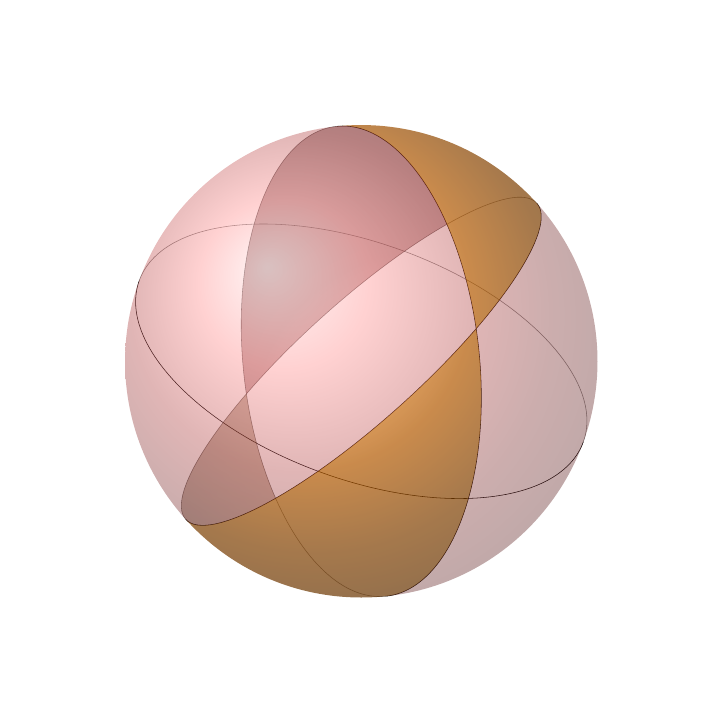
\begin{tikzpicture}[scale=3]
    \begin{scope}[rotate=-20]
      \draw [very thin, opacity=0.5] (1,0) arc [x radius=1, y radius=0.5, start angle=0, end angle=180];
      \draw [very thin] (1,0) arc [x radius=1, y radius=0.5, start angle=0, end angle=-180];
    \end{scope}
    \begin{scope}[rotate=42]
      \draw [very thin, opacity=0.5] (1,0) arc [x radius=1, y radius=0.25, start angle=0, end angle=180];
      \draw [very thin] (1,0) arc [x radius=1, y radius=0.25, start angle=0, end angle=-180];
    \end{scope}
    \begin{scope}[rotate=96]
      \draw [very thin, opacity=0.5] (1,0) arc [x radius=1, y radius=0.5, start angle=0, end angle=180];
      \draw [very thin] (1,0) arc [x radius=1, y radius=0.5, start angle=0, end angle=-180];
    \end{scope}
    \begin{scope}
      \clip [rotate=42] (1,0) arc [x radius=1, y radius=0.25, start angle=0, end angle=-180] -- (-1,-1) -- (1,-1) -- (1,0);
      \clip [rotate=96] (1,0) arc [x radius=1, y radius=0.5, start angle=0, end angle=-180] -- (-1,1) -- (1,1) -- (1,0);
      \shade [ball color = orange, opacity = 0.7] (0,0) circle [radius=1];
    \end{scope}
    \begin{scope}
      \clip [rotate=42] (1,0) arc [x radius=1, y radius=0.25, start angle=0, end angle=-180] -- (-1,1) -- (1,1) -- (1,0);
      \clip [rotate=96] (1,0) arc [x radius=1, y radius=0.5, start angle=0, end angle=-180] -- (-1,-1) -- (1,-1) -- (1,0);
      \shade [ball color = orange, opacity = 0.7] (0,0) circle [radius=1];
    \end{scope}
    \begin{scope}[transform canvas={rotate=180}, rotate=180]
      \clip [rotate=42] (1,0) arc [x radius=1, y radius=0.25, start angle=0, end angle=360];
      \clip [rotate=96] (1,0) arc [x radius=1, y radius=0.5, start angle=0, end angle=180] -- (-1,1) -- (1,1) -- (1,0);
      \shade [ball color = orange!50!black, opacity = 0.35] (0,0) circle [radius=1];
    \end{scope}
    \begin{scope}[transform canvas={rotate=180}, rotate=180]
      \clip [rotate=42] (1,0) arc [x radius=1, y radius=0.25, start angle=0, end angle=180] -- (-1,1) -- (1,1) -- (1,0);
      \clip [rotate=96] (1,0) arc [x radius=1, y radius=0.5, start angle=0, end angle=360];
      \shade [ball color = red!50!black, opacity = 0.35] (0,0) circle [radius=1];
    \end{scope}
    \begin{scope}
      \clip [rotate=96] (1,0) arc [x radius=1, y radius=0.5, start angle=0, end angle=-180] -- (-1,1) -- (1,1) -- (1,0);
      \clip [rotate=42] (1,0) arc [x radius=1, y radius=0.25, start angle=0, end angle=-180] -- (-1,1) -- (1,1) -- (1,0);
      \shade [ball color = red!60, opacity = 0.4] (0,0) circle [radius=1];
    \end{scope}
    \begin{scope}
      \clip [rotate=96] (1,0) arc [x radius=1, y radius=0.5, start angle=0, end angle=-180] -- (-1,-1) -- (1,-1) -- (1,0);
      \clip [rotate=42] (1,0) arc [x radius=1, y radius=0.25, start angle=0, end angle=-180] -- (-1,-1) -- (1,-1) -- (1,0);
      \shade [ball color = red!60, opacity = 0.4] (0,0) circle [radius=1];
    \end{scope}
  \end{tikzpicture}
  \vspace{-2em}
        \caption{Lunes on a sphere divide it into four parts.}
        \label{fig:lunes}
    \end{figure}
\end{question}
\end{tcolorbox}

\begin{tcolorbox}[title={Spherical Triangle Inequalities}]
    \begin{question}
        Prove that for any spherical triangle $ABC$ on a unit sphere with sides $a,b,c$ and angles $A,B,C$,
        \begin{enumerate}
            \item The triangle inequality holds: each side is smaller than the sum of the other two sides: 
            \begin{align*}
                a<b+c, \quad b<c+a, \quad c<a+b.
            \end{align*}
            \item Each side is larger than the difference of the other two sides.
            \item The sum of the sides of the triangle is positive and smaller than $2\pi$:
            \begin{align*}
                0<a+b+c<2\pi.
            \end{align*}
            \item The sum of the angles of the triangle is larger than $\pi$ and smaller than $3\pi$:
            \begin{align*}
                \pi<A+B+C<3\pi.
            \end{align*}
            \item The larger side of the triangle faces the larger angle of the spherical triangle.
            \item The following inequalities hold true for triangle's angles:
            \begin{align*}
                A+B-C<\pi,\quad A-B+C<\pi, \quad -A+B+C<\pi.
            \end{align*}
        \end{enumerate}
    \end{question}
\end{tcolorbox}
\begin{tcolorbox}[title={Congruent Spherical Triangles \& Gauss--Bonnet Theorem}]
    \begin{question}
        Remember from the Euclidean geometry that two plane triangles are \textbf{congruent} (having equal sides and angles) if (a) all three sides are equal (\textbf{SSS}), (b) two sides and the angle between them are equal (\textbf{SAS}), or (c) two angles and the side joining them are equal (\textbf{ASA}). However, two \textbf{incongruent} plane triangles may have all three angles equal to one another, simply because we can scale all sides of a plane triangle equally to get a triangle with larger/smaller sides but the same angles. Prove that for spherical triangles,
    \begin{enumerate}
        \item The three Euclidean criteria for congruent plane triangles (\textbf{SSS}, \textbf{SAS}, \textbf{ASA}) also hold true for spherical triangles.
        \item Two spherical triangles with equal angles (\textbf{AAA}) are congruent.
        \item Two congruent spherical triangles have equal areas.
        \item On a unit sphere, sum of triangle's angles equals $\pi$ plus the area of triangle:
        \begin{align*}
            A + B + C = \pi + (\text{area of }\triangle ABC).
        \end{align*}
    \end{enumerate}
    \end{question}
\end{tcolorbox}

\begin{tcolorbox}[title={Inverse Spherical Triangles}]
    \begin{question}
        Two spherical triangles $ABC$ and $A'B'C'$ have all their corresponding main elements equal to one another, that is,
        \begin{align*}
            A= A', \quad B=B',\quad C=C', \qquad
            a=a', \quad b=b',\quad c=c'.
        \end{align*}
        Prove that either the two triangles are \textbf{directly equal}, meaning one can be moved in space so that its vertices matches the vertices of the other triangle, or they are \textbf{inversely equal}, or simply \textbf{inverse} of each other, which means that they are reflections of each other with respect to a plane that passes through sphere's center.
        \begin{figure}[H]
            \centering
            \begin{tikzpicture}[scale=1.5]
               \pgfmathsetmacro\R{2} 
               % \fill[ball color=white!10, opacity=0.2] (0,0,0) circle (\R); % 3D lighting effect
                \filldraw[fill=white] (0,0,0) circle (\R cm);
                \foreach \angle[count=\n from 1] in {-5,225,290} {
                  \begin{scope}[rotate=\angle]
                    \path[draw,dashed,name path global=d\n] (2,0) arc [start angle=0,
                      end angle=180,
                      x radius=2cm,
                    y radius=1cm] ;
                    \path[draw,name path global=s\n] (-2,0) arc [start angle=180,
                      end angle=360,
                      x radius=2cm,
                    y radius=1cm] ;
                  \end{scope}
                }
                \InterSec{s1}{s2}{I3} ;
                \InterSec{s1}{s3}{I2} ;
                \InterSec{s3}{s2}{I1} ;
                %
                \fill[fill=red,opacity=0.5] (I1) to [bend right=8.5]  (I2) to [bend left=7] 
                (I3) to [bend left=6] (I1);
        
                \InterSec{d1}{d2}{J3} ;
                \InterSec{d1}{d3}{J2} ;
                \InterSec{d3}{d2}{J1} ;
                %\fill[blue] (J1)--(J2)--(J3)--cycle ;
        
                \fill[fill=blue,opacity=0.5] (J1) to [bend right=8.5]  (J2) to [bend left=7] 
                (J3) to [bend left=6] (J1);
        
              \end{tikzpicture}
            \caption{Inverse spherical triangles.}
            \label{fig:inverse}
        \end{figure}
    \end{question}
\end{tcolorbox}


\begin{tcolorbox}[title={Spherical Law of Cosines for Sides}]
    \begin{question}
        The cosine of one side of a spherical triangle is equal to the product of the cosine of the other two sides plus the product of sines of these two sides times the cosine of the angle between them:
        \begin{align*}
            \cos a &= \cos b \cos c + \sin b \sin c \cos A,\\
            \cos b &= \cos c \cos a + \sin c \sin a \cos B,\\
            \cos c &= \cos a \cos b + \sin a \sin b \cos C.
        \end{align*}
    \end{question}
\end{tcolorbox}


\begin{tcolorbox}
    \begin{question}
        Figure~\ref{fig:cosine} shows a spherical triangle $ABC$ with sides $a,b,c$ on a sphere centered at $O$. The tangent at $A$ to the arc $AB$ meets $OB$ at $D$ and the tangent at $A$ to the arc $AC$ meets $OC$ at $E$.
        \begin{figure}[H]
        \centering
                %%%% Spherical Cosine
        \def\xx{0.5} % reduction x axis, cavalier perspective
        \def\aa{30}  % angles AOB=BOC
        \def\r {3}   % radius
        \def\l {4.5} % distance AD=AE
        \pgfmathsetmacro\ay{\r*cos(\aa)} % Coordinates A
        \pgfmathsetmacro\az{\r*sin(\aa)} 
        \pgfmathsetmacro\cx{\r*sin(\aa)} % Coordinates C
        \pgfmathsetmacro\cy{\r*cos(\aa)} 
        \pgfmathsetmacro\nx{-sin(\aa)*cos(\aa)} % normal vector OAC plane
        \pgfmathsetmacro\ny{ sin(\aa)*sin(\aa)}
        \pgfmathsetmacro\nn{sqrt(2*\nx*\nx+\ny*\ny)} % modulus
        \pgfmathsetmacro\ap{acos(abs(\nx)/\nn)} % angle between planes XY and OAC
        \begin{tikzpicture}[scale=2,line cap=round,line join=round,x={(-\xx cm,-\xx cm)},y={(1 cm,0 cm)},z={(0 cm,1 cm)}]
            
          % coordinates
          \coordinate (O) at (0,0,0);
          \coordinate (A) at (0,\ay,\az);
          \coordinate (B) at (0,\r,0);
          \coordinate (C) at (\cx,\cy,0);
          \coordinate (D) at (0,\l,0);
          \coordinate (E) at ({\l*sin(\aa)},{\l*cos(\aa)},0);
          \filldraw[fill=white] (O) -- (A) -- (D) -- (E) -- cycle;
          % labels
          \node      at (O) [left]  {$O$};
          \node      at (A) [above] {$A$};
          \node      at (B) [below right] {$B$};
          \node      at (C) [below left] {$C$};
          \node      at (D) [right] {$D$};
          \node      at (E) [below right] {$E$};
          \node[red] [label={[label distance=0.1cm,color=red]-90:$a$}] at ($(B)!0.5!(C)$) [below] {};
          \node[red] at ($(A)!0.5!(C)$)         {$b$};
          \node[red] [label={[label distance=0.1cm,color=red]30:$c$}] at ($(A)!0.7!(B)$) [right] {};
          % spheric triangle
          \begin{scope} [canvas is xy plane at z=0]
            \clip (O) -- (D) -- (E) -- cycle;
            \draw[red] (O) circle (\r);
          \end{scope}
          \begin{scope}[canvas is yz plane at x=0]
            \clip (O) -- (A) -- (D) -- cycle;
            \draw[red] (O) circle (\r);
          \end{scope}
          \begin{scope}[rotate around z=-\aa, rotate around y=\ap-90,canvas is yz plane at x=0]
            \clip (O) -- (A) -- (E) -- cycle;
            \draw[red] (O) circle (\r);
          \end{scope}
          % lines
          \draw (O) -- (A) -- (D) -- (E) -- cycle;
          \draw[dashed] (O) -- (D);
          \draw (A) -- (E);
        \end{tikzpicture}
        \caption{Spherical triangle $ABC$ with tangents to arcs at vertex $A$.}
        \label{fig:cosine}
    \end{figure}
    \begin{enumerate}
            \item  Using the Law of Cosines in the plane, show that
        \begin{align*}
            \displaystyle \cos A = \frac{\cos a - \cos b \cos c}{\sin b \sin c}.
        \end{align*}
        \item Using the Pythagorean identity $\sin^2 A + \cos^2 A = 1$, prove that
        \begin{align*}
            \displaystyle \sin A = \frac{\sqrt{1-\cos^2 a - \cos^2 b - \cos^2 c + 2\cos a \cos b \cos c}}{\sin b \sin c}.
        \end{align*}
    \end{enumerate}
    \end{question}
\end{tcolorbox}

\begin{tcolorbox}[title={Spherical Law of Sines}]
    Consider the ratio between the sine of an angle and the sine of its opposite side in a spherical triangle. Prove that this ratio is the same for all three angles:
    \begin{align*}
        \frac{\sin A}{\sin a} = \frac{\sin B}{\sin b} = \frac{\sin C}{\sin c}.
    \end{align*}
\end{tcolorbox}

\begin{tcolorbox}[title={Five--Piece Spherical Trigonometric Identities}]
In a spherical triangle $ABC$ with side-lengths $a,b,c$, prove the five-piece identities:
    \begin{question}[name=Side's Sine Times Adjacent Angle's Cosine]
    For any side $x$ and angle $Y$ adjacent to it, the product $\sin x \cos Y$ equals $\cos y \sin z$ \textbf{minus} $\sin y \cos z \cos X$:
        \begin{align*}
        \text{Side } a: \begin{cases}
            \sin a \cos B = \cos b \sin c - \sin b \cos c \cos A,\\
            \sin a \cos C = \cos c \sin b - \sin c \cos b \cos A,            
        \end{cases}\\
        \text{Side } b: \begin{cases}
            \sin b \cos C = \cos c \sin a - \sin c \cos a \cos B,\\
            \sin b \cos A = \cos a \sin c - \sin a \cos c \cos B,\\
        \end{cases}\\
        \text{Side } c: \begin{cases}
            \sin c \cos A = \cos a \sin b - \sin a \cos b \cos C,\\ 
            \sin c \cos B = \cos b \sin a - \sin b \cos a \cos C.
        \end{cases}
        \end{align*}
    \end{question}
    \begin{question}[name=Angle's Sine Times Adjacent Side's Cosine]
    For any angle $X$ and side $y$ adjacent to it, the product $\sin X \cos y$ equals $\cos Y \sin Z$ \textbf{plus} $\sin Y \cos Z \cos x$:
        \begin{align*}
        \text{Angle } A: \begin{cases}
            \sin A \cos b = \cos B \sin C + \sin B \cos C \cos a,\\
            \sin A \cos c = \cos C \sin B + \sin C \cos B \cos a,\\ 
        \end{cases}\\
        \text{Angle } B: \begin{cases}
            \sin B \cos c = \cos C \sin A + \sin C \cos A \cos b,\\
            \sin B \cos a = \cos A \sin C + \sin A \cos C \cos b,\\
        \end{cases}\\
        \text{Angle } C: \begin{cases}
            \sin C \cos a = \cos A \sin B + \sin A \cos B \cos c,\\
            \sin C \cos b = \cos B \sin A + \sin B \cos A \cos c.
        \end{cases}
        \end{align*}
    \end{question}
\end{tcolorbox}

\begin{tcolorbox}[title={Spherical Law of Cosines for Angles}]
    \begin{question}
        The cosine of an angle of a spherical triangle equals the product of sines of the other two angles and the cosine of the side between them \textbf{minus} the product of cosines of the other two angles:
    \begin{align*}
        \cos A &= \sin B \sin C \cos a - \cos B \cos C,\\
        \cos B &= \sin C \sin A \cos b - \cos C \cos A,\\
        \cos C &= \sin A \sin B \cos c - \cos A \cos B.
    \end{align*}
    \end{question}
    \begin{question}
        Imply that
        \begin{align*}
            \cos a &= \frac{\cos A + \cos B\cos C}{\sin B \sin C},\\
            \sin^2\frac{a}{2} &= -\frac{\cos A + \cos(B+C)}{2\sin B \sin C}. 
        \end{align*}
    \end{question}
\end{tcolorbox}


\begin{tcolorbox}[title={Half--Angle and Half--Side Spherical Formulas}]
    \begin{question}
        For every spherical triangle $ABC$ with angles $A,B,C$ and $a,b,c$, let $p$ be the semiperimeter: $p=(a+b+c)/2$. Prove the following half--angle trigonometric formulas:
    \begin{enumerate}
        \item $\displaystyle \sin^2\frac{A}{2} = \frac{\sin\left(\frac{a+b-c}{2}\right)\sin\left(\frac{a-b+c}{2}\right)}{\sin b \sin c}$,
        \item $\displaystyle \sin^2\frac{A}{2} = \frac{\sin(p-b)\sin(p-c)}{\sin b \sin c}$,
        \item $\displaystyle \cos^2\frac{A}{2} = \frac{\sin p\sin(p-a)}{\sin b \sin c}$,
        \item $\displaystyle \tan^2\frac{A}{2} = \frac{\sin(p-b)\sin(p-c)}{\sin p\sin(p-a)}$,
        \item $\displaystyle \sin A = \frac{2\sqrt{\sin p \sin(p-a)\sin(p-b)\sin(p-c)}}{\sin b \sin c}$.
    \end{enumerate}
    \end{question}
    \begin{question}
        For every spherical triangle $ABC$ with angles $A,B,C$ and $a,b,c$, define $P=(a+b+c)/2$. Prove the following half--side trigonometric identities:
    \begin{enumerate}
        \item $\displaystyle \sin^2\frac{a}{2} = -\frac{\cos P\cos(P-A)}{\sin B \sin C}$,
        \item $\displaystyle \cos^2\frac{a}{2} = \frac{\cos(P-B)\cos(P-C)}{\sin B \sin C}$,
        \item $\displaystyle \tan^2\frac{a}{2} = -\frac{\cos P \cos(P-A)}{\cos(P-B)\cos(P-c)}$,
        \item $\displaystyle \sin a = \frac{2\sqrt{-\cos P \cos(P-A)\cos(P-B)\cos(P-C)}}{\sin B \sin C}$.
    \end{enumerate}
    \end{question}
\end{tcolorbox}

\begin{tcolorbox}[title={Spherical Law of Haversines}]
    \begin{definition}
        Some hundreds of years ago when spherical trigonometry was a hot-topic for mathematicians, there was another periodic function besides cosine and sine, called \textbf{versine}, short for \textbf{versed sine}, defined by $\text{versin}(\theta)=1-\cos \theta$.
    \end{definition}
    \begin{definition}
        Since $1-\cos\theta=2\sin^2\theta$, it makes sense to define a \textbf{halved versed sine}, or shortly, \textbf{haversine}, by $\text{hav}(\theta)=\sin^2\left(\frac{\theta}{2}\right)$.
    \end{definition}
    \begin{question}\label{q:hav}
        Prove the \textbf{Haversine Formula} in a spherical triangle $ABC$ with side-lengths $a,b,c$:
        \begin{align*}
            \text{hav}(c) = \text{hav}(a-b) +\sin(a) \sin(b) \  \text{hav}(C). 
        \end{align*}
    \end{question}
\end{tcolorbox}

\begin{tcolorbox}[title={Swimming the Depths of the Algebraic Ocean}]
    Kaywañan is an Algebra Competition, and you may say its motto is ``Let No One Ignorant of Algebra Enter.''  So far, we have been vigorously forging algebraic equations and definitions that are deeply rooted within their applications. It is both an intention and a purpose of Kaywañan to be defined as the collection of most important algebraic equations and identities that one may encounter in dealing with in ordinary, Euclidean flatland geometry, as well as non-Euclidean monsters and witches that might appear in hyperbolic geometry. \\
    \\
    We have not even started to discuss the geometry of hyperbola and its associated hyperboloid. The most advanced formula, I would say, in Kaywañan so far is that of Problem~\ref{q:hav}, the Spherical Law of Haversines, which has absolutely fascinating applications in astronomy. The haversine formula for spherical triangles is just an example of myriads of unknown equations in Spherical Geometry, the most special type of Elliptic Geometry. You can only imagine how many more of such algebraic equations may be found, written down, and added to Kaywañan if we consider other elliptic structures than the Sphere, such as the Ellipsoid.\\
    \\
    There are other types of non-Euclidean geometries that some might say are even more surprising than the fact that angles of a spherical triangle add up to more than $\pi$. If the Euclidean plane is not infinite in all directions, and in the special case when the plane is limited to a $1\times 1$ Square of the Euclidean Plane, you can imagine that the corresponding points on opposite sides of the square are actually the same point, as if you map the surface of a doughnut to the $1\times 1$ Euclidean Square. If we start walking from a certain point in any of the two directions of the Euclidean Square on the surface of a doughnut, we would reach the same point. The same would happen if we map the sphere to the Euclidean plane, but the surface of the doughnut and that of a sphere are clearly distinct to us. If we had no idea of the third dimension, as if we were ants walking around in two-dimensional Euclidean plane, we would never even be able to know whether the surface on which we walk is a doughnut or a sphere.\\
    \\
    Here, at the depths of the Algebraic Ocean of Kaywañan, Titan, Moon of Saturn, where we can see the positive curvature of the surface of the core of Titan, nobody doubts the spherical shape of Planet of Algebra, Kaywan. There are rumours that in earlier Eons, Kaywañans (those who live around Saturn) believed that Titan is the most special place in the S\"olar System, and after one of them dreamed of Maurits Cornelis Escher's ``Angels and Devils'' painting, they started to preach a certain belief in a Hyperbolic Geometry of Titan to emphasize their uniqueness among moons of Saturn and other celestial objects.\\
    \\
    It is now, however, a ridiculous claim to believe in a hyperbolic geometry for the actually spherical surface of Titan, maybe as ridiculous as believing in a Flat Earth once you have traveled to the moon and seen the biosphere of the Earth from afar. Now that we can swim the depths of Kaywañan and measure the spherical arcs close to the core of Titan, hyperbolic beliefs are but a joke. We may study mythology of such treacheries in the advanced levels of Napirañan Geometry Contest, but here in Kaywañan we stick to the algebra.
\end{tcolorbox}


\begin{tcolorbox}[title={Maclaurin Series of Versine \& Haversine}]
    \begin{question}
        Prove that for any complex number $z$,
        \begin{align*}
            \text{versin}(z) = \sum _{k=1}^{\infty }{\frac {(-1)^{k-1}z^{2k}}{(2k)!}} \quad \text{and} \quad \text{hav}(z) = \sum _{k=1}^{\infty }{\frac {(-1)^{k-1}z^{2k}}{2(2k)!}}.
        \end{align*}
        Then show that the limit of both $\text{versin}(\theta)/\theta$ and $\text{hav}(\theta)/\theta$ when $\theta \to 0$ is $0$.
    \end{question}
\end{tcolorbox}


\begin{tcolorbox}[title={The Sine Formulae (from ``Spherical Astronomy'')}]
The following method of notation is quoted from ``Textbook on Spherical Astronomy'' by W. M. Smart and R. M. Green, given in the first chapter as one of the main formulas (formulae \textbf{A} and \textbf{D}) in Spherical Trigonometry.%\footnote{The name ``Laterangular'' is not used in the book, though.}
    \begin{definition}[Laterangular Function of a Spherical Triangle]
    For any spherical triangle $ABC$, the \textbf{Laterangular Function of $A$}, denoted $X(a,A)$, is defined by
        \begin{align*}
            \left(X(a,A)\right)^2\cdot \sin^2 a \sin^2 b \sin^2 c = 1- \cos^2 a -\cos^2 b -\cos^2 c + 2\cos a \cos b \cos c.
        \end{align*}
    \end{definition}
    \begin{question}
    In a spherical triangle $ABC$ with side-lengths $a,b,c$,
            \begin{enumerate}
            \item  Prove the \textbf{Astronomical Sine} formula:
            \begin{align*}
                \sin^2 b \cdot \sin^2 c \cdot \sin^2 A &= 1- \cos^2 a -\cos^2 b - \cos^2 c + 2\cos a \cos b \cos c.
            \end{align*}
            \item Prove that
            \begin{align*}
                \left(X(a,A)\right)^2 &= \left(\frac{\sin A}{\sin a}\right)^2,
            \end{align*}
            and imply that the Laterangular Function must be symmetric, so that $X(a,A) = X(b,B) = X(c,C)$.
            \item If all main elements of triangle $ABC$ are smaller than $\pi$, then the \textbf{Spherical Law of Sines} holds true:
            \begin{align*}
                \frac{\sin A}{\sin a} =  \frac{\sin B}{\sin b} = \frac{\sin C}{\sin c} = \frac{\sqrt{ 1- \cos^2 a -\cos^2 b - \cos^2 c + 2\cos a \cos b \cos c}}{\sin a \sin b \sin c}.
            \end{align*}
            \end{enumerate}
    \end{question}
    \begin{definition}[Four--Piece Spherical Trigonometric Terminology]
        In the spherical triangle $ABC$ consider the four consecutive parts $B,a,C,b$. The angle $C$ is contained by the two sides $a$ and $b$ and is called the \textbf{inner angle}. The side $a$ is flanked by the two angles $B$ and $C$ and is called the \textbf{inner side}.
    \end{definition}
    \begin{question}[name={Four-Part Identity}]
        Prove that $\cos(\text{inner side})\cdot \cos(\text{inner angle})$ equals
        \begin{align*}
            \sin(\text{inner side})\cdot \cot(\text{other side}) - \sin(\text{inner angle})\cdot \cot(\text{other angle}).
        \end{align*}
    \end{question}    
\end{tcolorbox}


\begin{tcolorbox}[title={Delambre's and Napier's Analogies}]
    \begin{question}[name={Delambre's Aanlogies}]
        In a spherical triangle $ABC$ with sides $a,b,c$,
        \begin{align*}
            \sin\frac{c}{2}\sin\frac{A-B}{2} = \cos\frac{C}{2}\sin\frac{a-b}{2} \quad \text{and} \quad
            \sin\frac{c}{2}\cos\frac{A-B}{2} = \sin\frac{C}{2}\sin\frac{a+b}{2},\\
            \cos\frac{c}{2}\sin\frac{A+B}{2} = \cos\frac{C}{2}\cos\frac{a-b}{2} \quad \text{and} \quad
            \cos\frac{c}{2}\cos\frac{A+B}{2} = \sin\frac{C}{2}\cos\frac{a+b}{2}.
        \end{align*}
    \end{question}
\end{tcolorbox}

\noindent Taking Delambre's equations, which are also called \textbf{Gauss's Spherical Equations}, in pairs, we obtain Napier's Analogies:

\begin{tcolorbox}[title={Napier's Analogies}]
\begin{question}[name={Napier's Aanlogies}]
        In a spherical triangle $ABC$ with sides $a,b,c$,
        \begin{align*}
            \tan\frac{a+b}{2} = \frac{\displaystyle\cos\frac{A-B}{2}}{\displaystyle\cos\frac{A+B}{2}}\tan\frac{c}{2} \quad \text{and} \quad
            \tan\frac{a-b}{2} = \frac{\displaystyle\sin\frac{A-B}{2}}{\displaystyle\sin\frac{A+B}{2}}\tan\frac{c}{2},\\
            \tan\frac{A+B}{2} = \frac{\displaystyle\cos\frac{a-b}{2}}{\displaystyle\cos\frac{a+b}{2}}\cot\frac{C}{2} \quad \text{and} \quad
            \tan\frac{A-B}{2} = \frac{\displaystyle\sin\frac{a-b}{2}}{\displaystyle\sin\frac{a+b}{2}}\cot\frac{C}{2}.
        \end{align*}
    \end{question}
\end{tcolorbox}




\begin{tcolorbox}[title={Napier's Rules}]
    \begin{question}[name={Napier's Rules for Right Spherical Triangles}]
        If one main element among $a,b,c,A,B,C$ is $\pi/2$, there would be five remaining unknown parts. John Napier suggested Five--Piece Mnemonics shown in Figures~\ref{fig:napierfive1} and \ref{fig:napierfive2} [from \href{https://en.wikipedia.org/wiki/File:Spherical_trigonometry_Napier_right-angled.svg}{Wikipedia}] to prove:
        \begin{figure}[H]
            \centering
            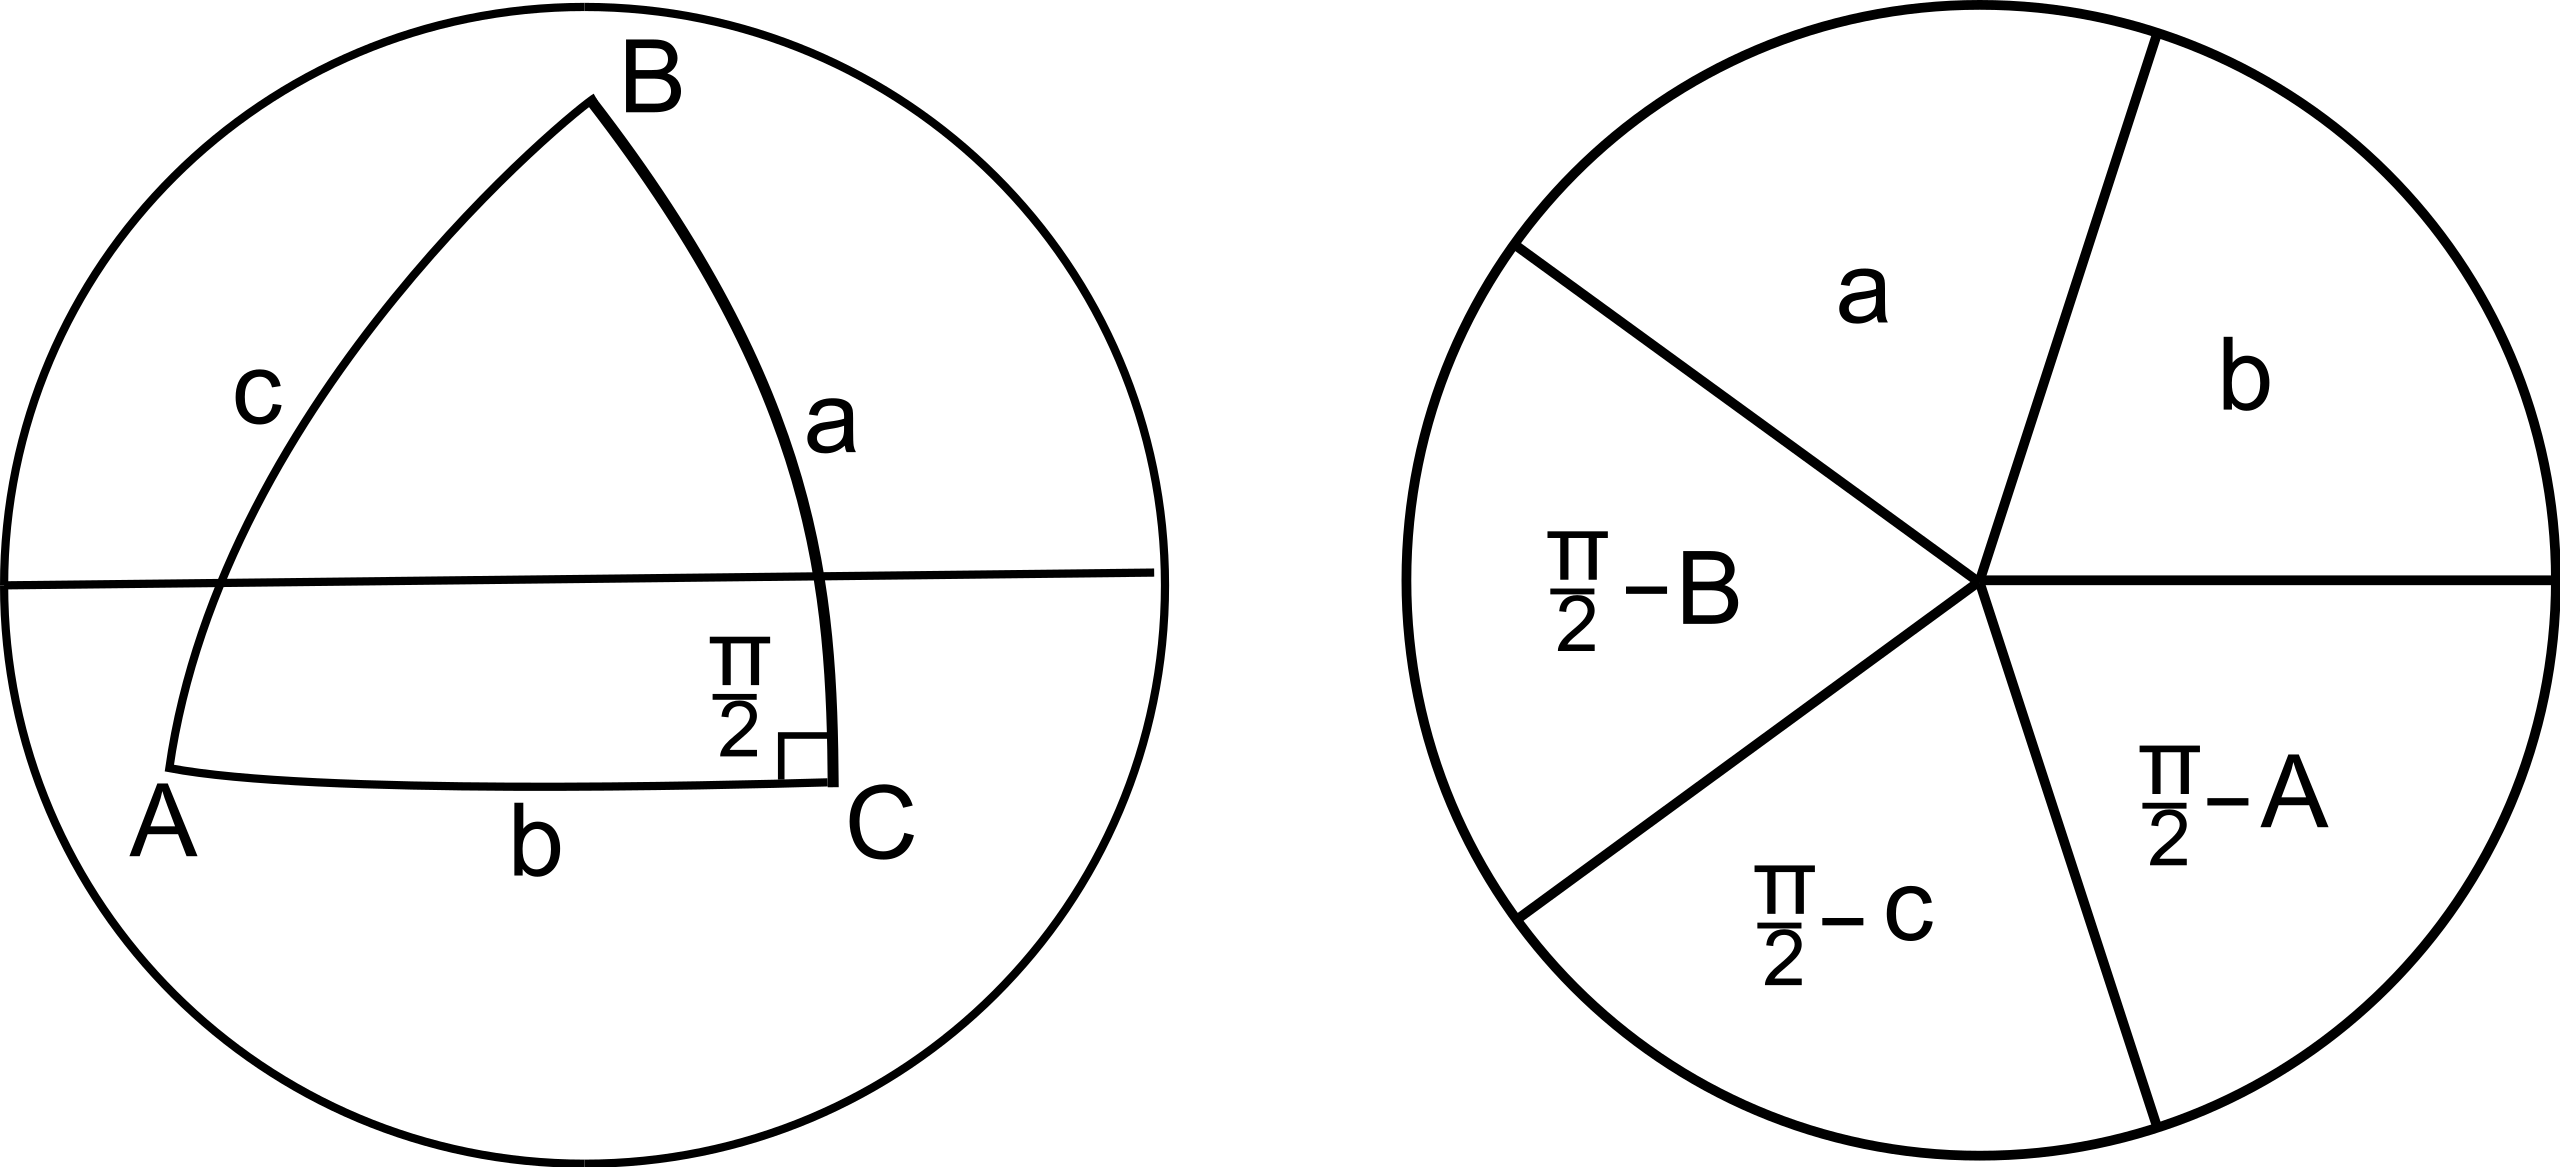
\includegraphics[width=0.6\textwidth]{IMG/Napier.png}
            \caption{Napier's Mnemonics (When One Angle is Right)}
            \label{fig:napierfive1}
        \end{figure}
        \begin{enumerate}
            \item The sine of any middle part equals the product of tangents of adjacent parts.
            \item The sine of any middle part equals the product of cosines of opposite parts.
        \end{enumerate}
    \end{question}
\end{tcolorbox}

% \begin{figure}[H]
%     \centering
%     \begin{subfigure}[b]{0.45\textwidth}
%     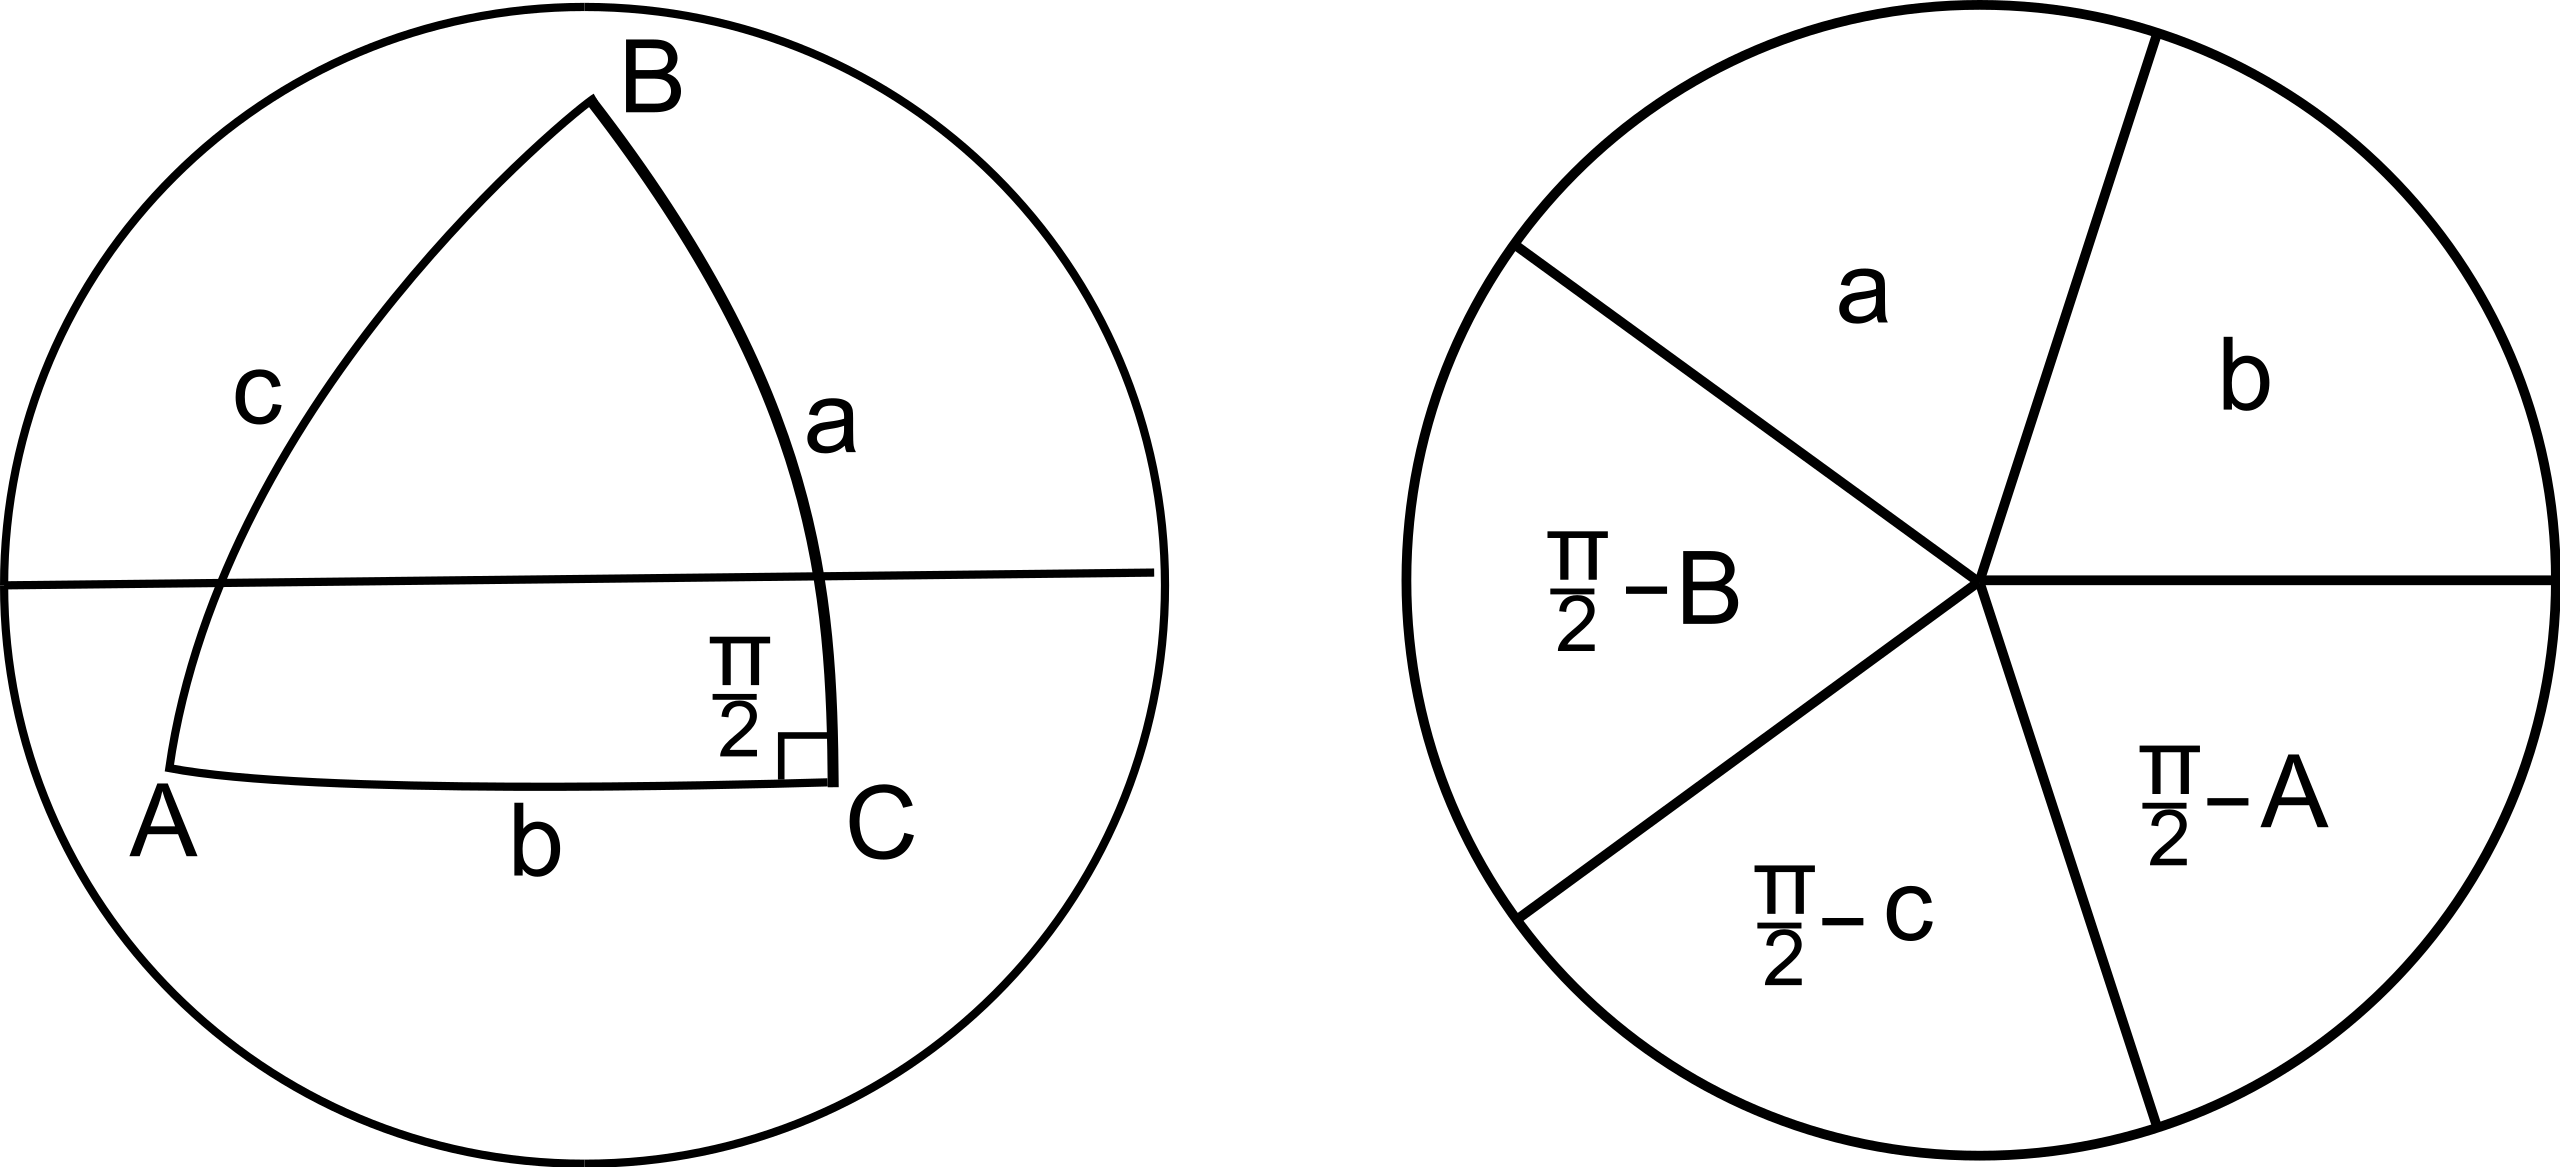
\includegraphics[width=\textwidth]{IMG/Napier.png}
%     \caption{When One Angle is Right }
%     \label{fig:napierfive1}
%     \end{subfigure}
%     \hfill
%     \begin{subfigure}[b]{0.45\textwidth}
%     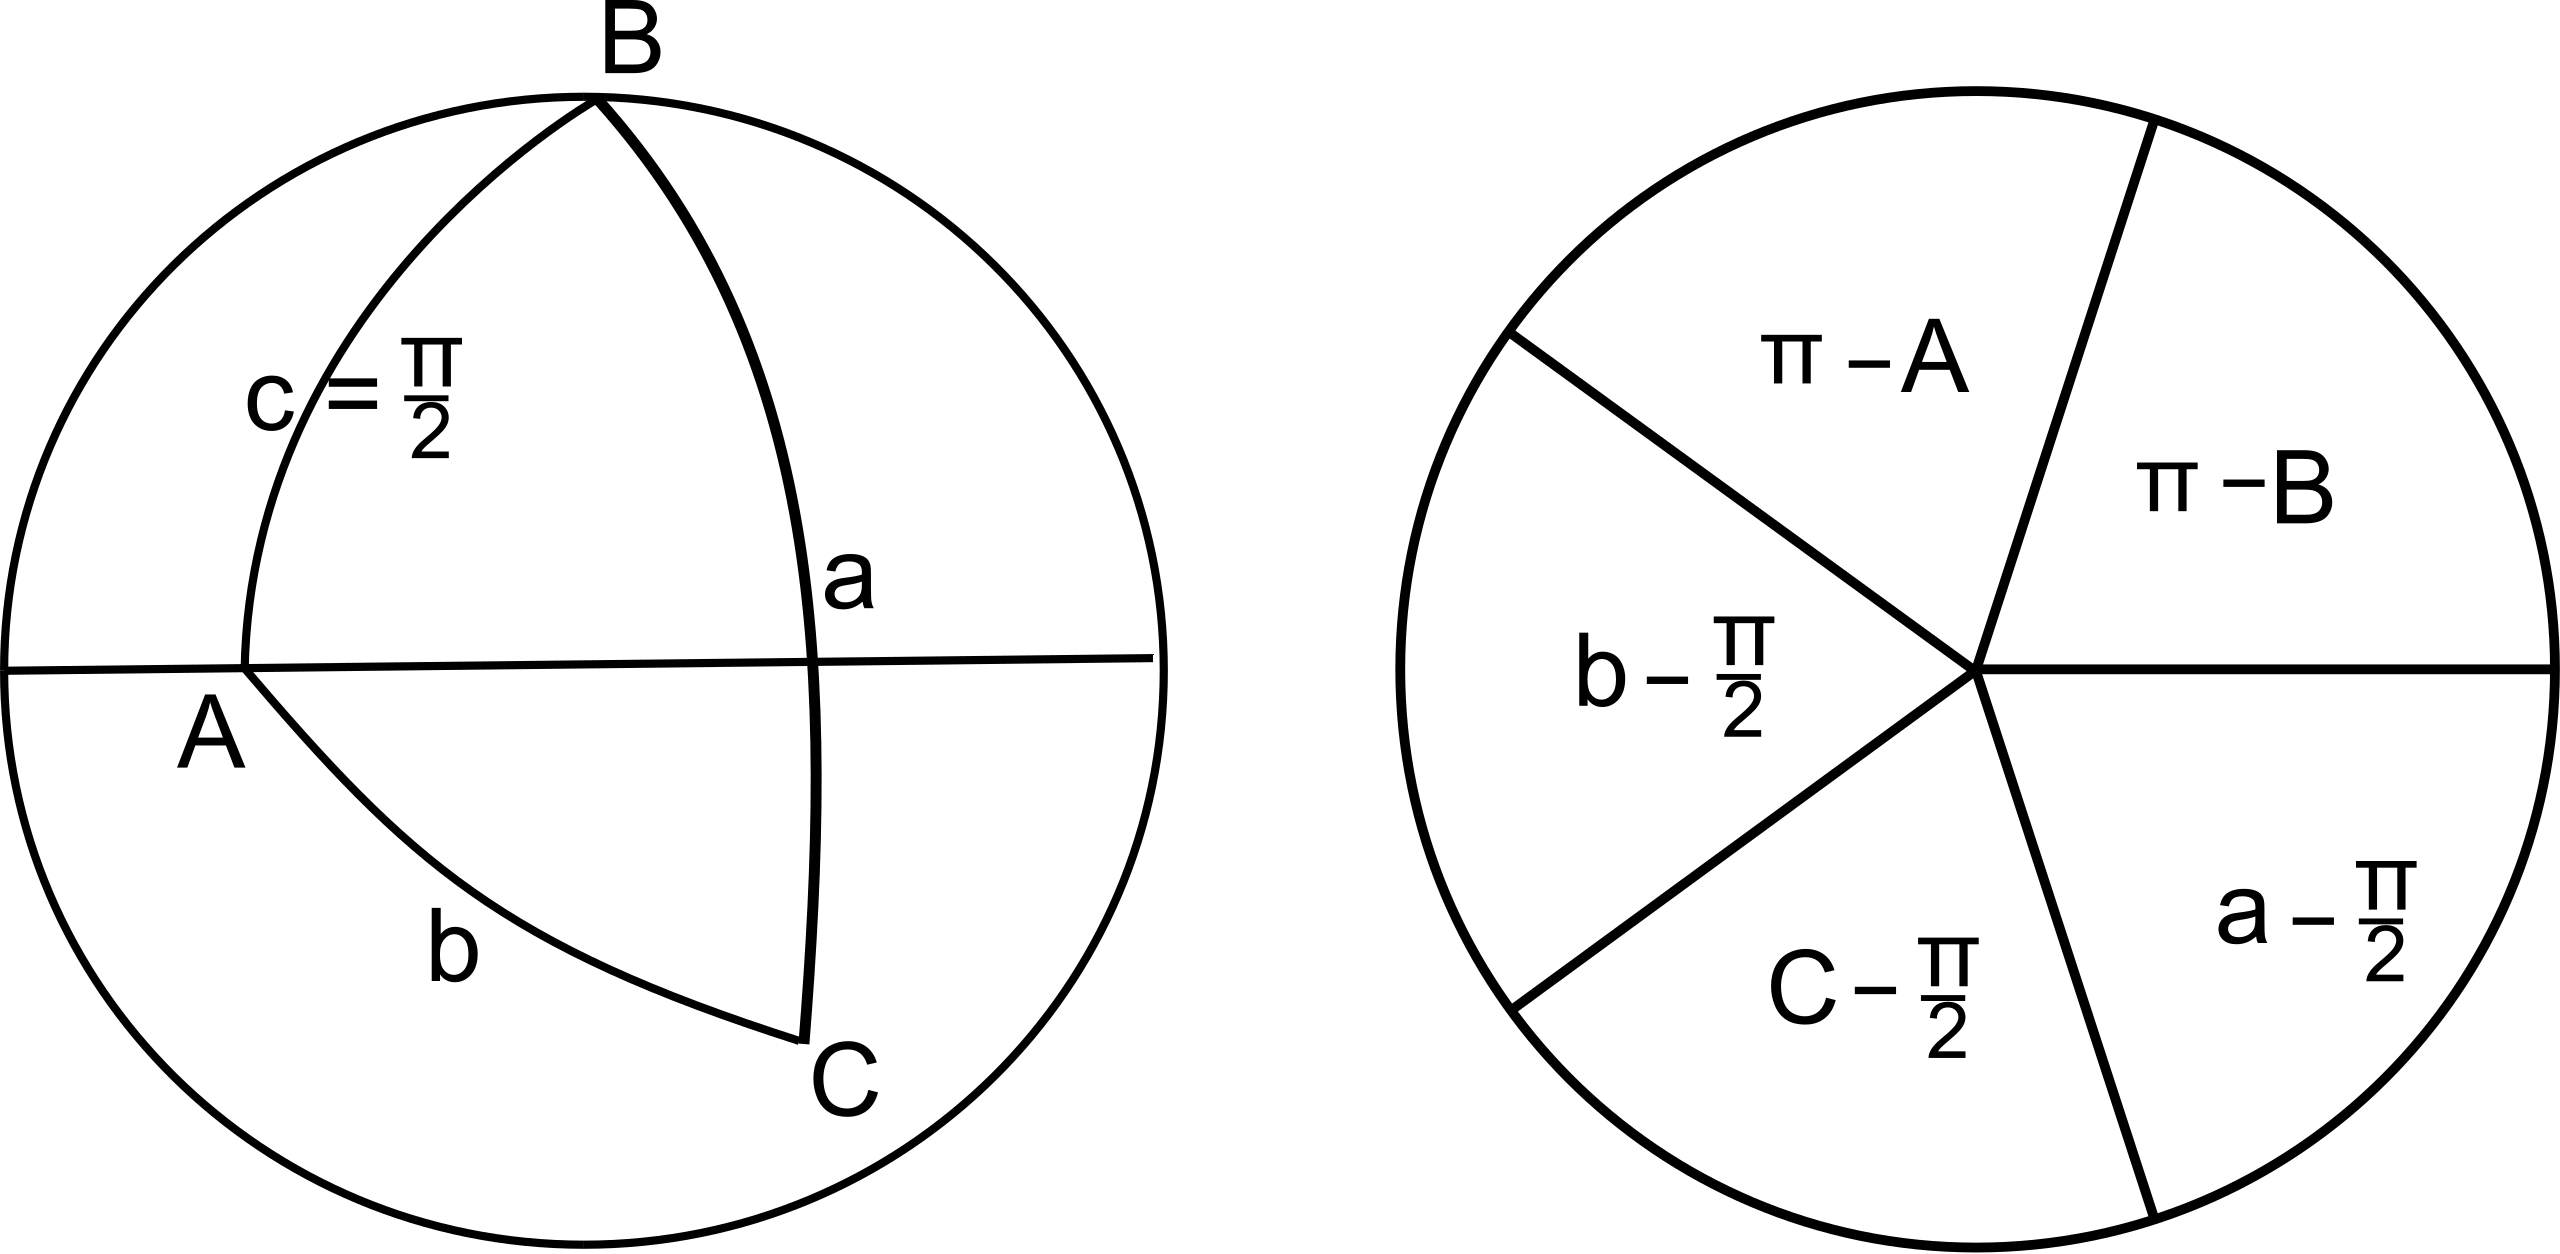
\includegraphics[width=\textwidth]{IMG/Napier2.png}
%     \caption{When One Side is a Quadrant}
%     \label{fig:napierfive2}
%      \end{subfigure}
%      \caption{Napier's Five--Piece Mnemonics [\href{https://en.wikipedia.org/wiki/File:Spherical_trigonometry_Napier_right-angled.svg}{Wikipedia (a)} \& \href{https://commons.wikimedia.org/wiki/File:Spherical_trigonometry_Napier_quadrantal_01.svg}{(b)}]}
%      \label{fig:napierfive}
% \end{figure}

\begin{tcolorbox}[title={Napier's Ten Right Spherical Triangle Commandments}]
    \begin{question}[name={Napier's Ten Commandments}]
        For any spherical triangle $ABC$ with a right angle at $A$, Napier's Ten Rules are the ten equations derived from various spherical trigonometric identities studied in previous problems [\href{https://commons.wikimedia.org/wiki/File:Spherical_trigonometry_Napier_quadrantal_01.svg}{Wikipedia}]:
        
    \begin{figure}[H]
        \centering
        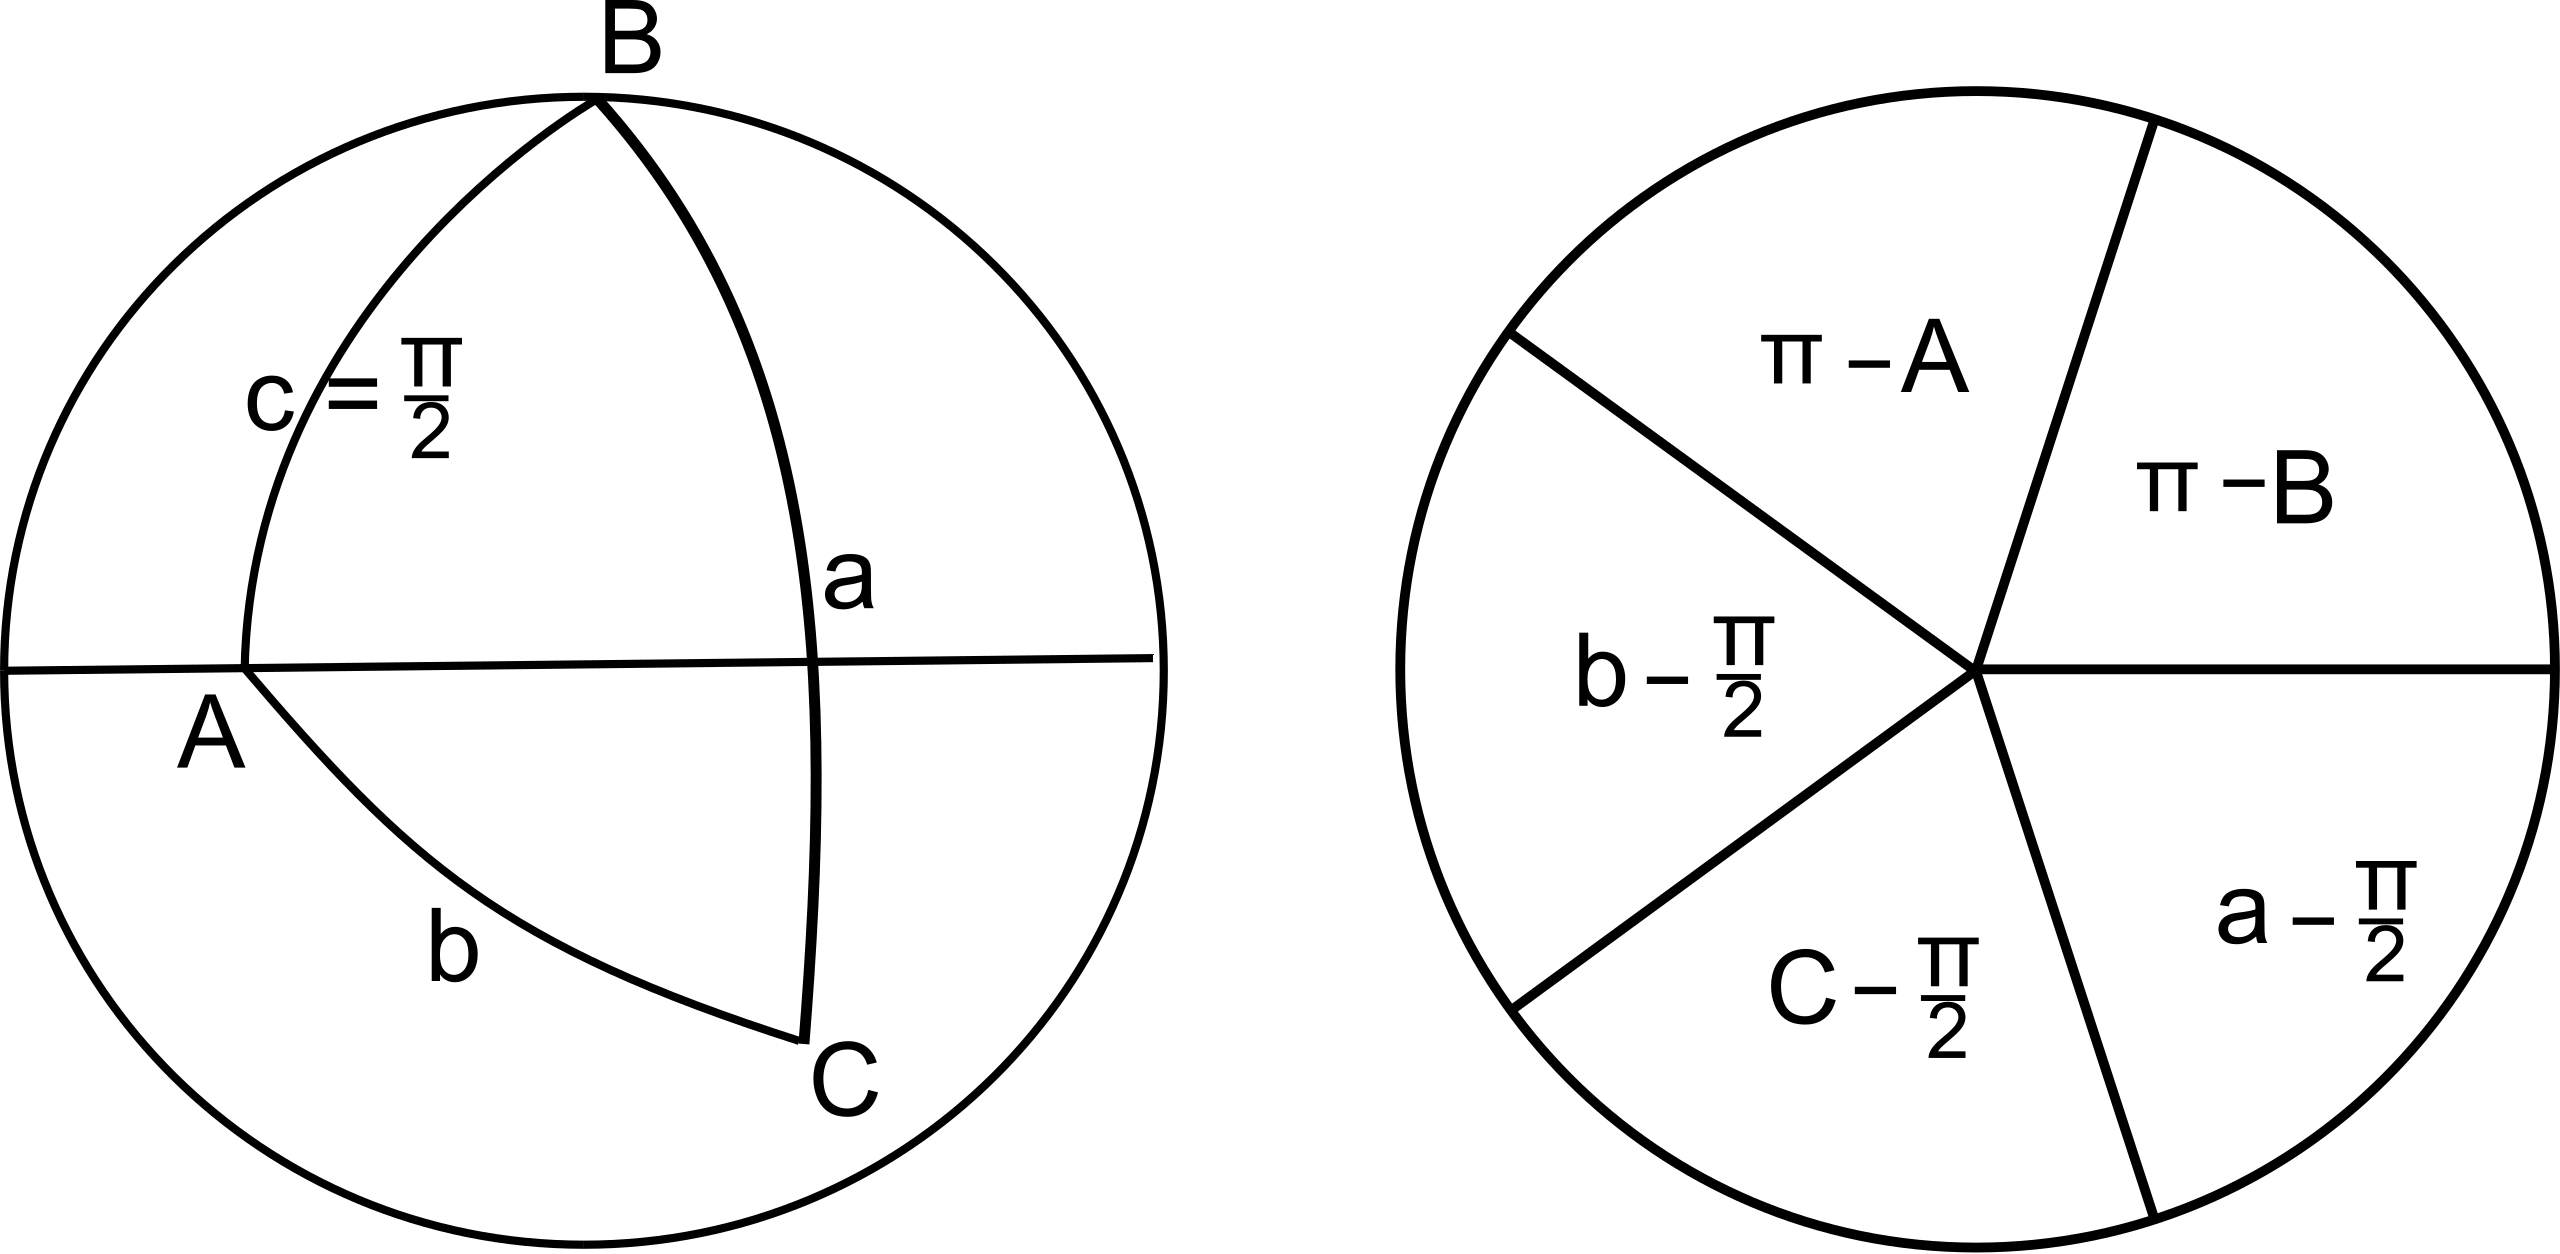
\includegraphics[width=0.6\textwidth]{IMG/Napier2.png}
        \caption{Napier's Mnemonics (When One Side is a Quadrant)}
        \label{fig:napierfive2}
    \end{figure}

    \begin{enumerate}
            \item[\color{green}(I)] $\color{green} \cos a = \cos b \cos c$, A.K.A. \textit{\color{green} Spherical Pythagorean Theorem},
            \item[\color{blue}(II)] $\color{blue} \sin b = \sin a \sin B$, derived from \textit{Spherical Law of Sines},
            \item[\color{blue}(III)] $\color{blue} \sin c = \sin a \sin C$, also from \textit{Spherical Law of Sines},
            \item[\color{red}(IV)] $\color{red} \cos B = \cos b \sin C$, by \textit{Spherical Law of Cosines for Angle $B$},
            \item[\color{red}(V)] $\color{red} \cos C = \cos c \sin B$, also by \textit{Spherical Law of Cosines}, but for Angle $C$,
            \item[\color{red}(VI)] $\color{red} \cos a = \cot B \cot C$, by \textit{Spherical Law of Cosines for Angle $A$},
            \item[\color{teal}(VII)] $\color{teal} \cos B = \cot a \tan c$, by \textit{Napier's Four--Part Identity} for $\cos c \cos B$,
            \item[\color{teal}(VIII)]$\color{teal} \cos C = \tan b \cot a$, by \textit{Napier's Four--Part Identity} for $\cos b \cos C$,
            \item[\color{teal}(IX)]  $\color{teal} \sin b = \tan c \cot C$, by \textit{Napier's Four--Part Identity} for $\cos b \cos A$,
            \item[\color{teal}(X)] $\color{teal} \sin c = \cos c \sin B$, by \textit{Napier's Four--Part Identity} for $\cos c \cos A$.
        \end{enumerate}
    \end{question}
    
    \vspace{-1em}
    
    \begin{question}
        Prove that Napier's Ten Commandments can be reduced to the following cosine formulae by changing $b$ and $c$ to $\frac{\pi}{2}-b$ and $\frac{\pi}{2}-c$, respectively:
        \begin{tasks}(2)
            \task $\displaystyle\cos a = \sin\left(\frac{\pi}{2}-b\right)\sin\left(\frac{\pi}{2}-c\right)$,
            \task $\displaystyle\cos a = \cot B \cot C$,
            \task $\displaystyle\cos \left(\frac{\pi}{2}-b\right) = \sin a \sin B$,
            \task $\displaystyle\cos \left(\frac{\pi}{2}-b\right) = \cot \left(\frac{\pi}{2}-c\right) \cot C$,
            \task $\displaystyle\cos \left(\frac{\pi}{2}-c\right) = \sin a \sin C$,
            \task $\displaystyle\cos \left(\frac{\pi}{2}-c\right) = \cot \left(\frac{\pi}{2}-b\right) \cot B$,
            \task $\displaystyle\cos B = \sin \left(\frac{\pi}{2}-b\right) \sin C$,
            \task $\displaystyle\cos B = \cot a \cot \left(\frac{\pi}{2}-c\right)$,
            \task $\displaystyle\cos C = \sin \left(\frac{\pi}{2}-c\right) \sin B$,
            \task $\displaystyle\cos C = \cot \left(\frac{\pi}{2}-b\right) \cot a$.
        \end{tasks}
        Napier's Ten Commandments and their ten cosine forms formulae inspired Napier to make his \textbf{Napier Rules for Right Spherical Triangles}.
    \end{question}
\end{tcolorbox}

\begin{tcolorbox}[title={The Global Half--Side Identities}]
\begin{definition}[Half--Side Spherical Triangle Identities] 
    For any spherical triangle $ABC$, the \textbf{Halveside Function of $A$}, denoted $H(a,A)$, is defined by
        \begin{align*}
            H(a,A)\cdot\cos(P-A)&=\tan \left({\frac {a}{2}}\right).
        \end{align*}
    where $P=(A+B+C)/2$.
    \end{definition}
    \begin{question}
    In a spherical triangle $ABC$ with side-lengths $a,b,c$,
            \begin{enumerate}
            \item  Prove the \textbf{Astronomical Half--Side Tangent} formula:
            \begin{align*}
                \tan \left({\frac {a}{2}}\right)&={\sqrt {\frac {-\cos P}{\cos(P-A)\cos(P-B)\cos(P-C)}}}\cos(P-A),
            \end{align*}
            \item Prove that
            \begin{align*}
                \left(H(a,A)\right)^2 &= \frac {-\cos P}{\cos(P-A)\cos(P-B)\cos(P-C)},
            \end{align*}
            and imply that the Laterangular Function must be symmetric, so that $H(a,A) = H(b,B) = H(c,C)$.
            \item Prove \textbf{Mollweide's} formula in Euclidean plane:
            \begin{align*}
                \displaystyle \left(\tan \frac{A}{2}\right )^{2}=\frac {(a+b-c)(a-b+c)}{(a+b+c)(-a+b+c)}.
            \end{align*}
            \end{enumerate}
    \end{question}
    \begin{question}[name={Spherical Half--Side Tangent--Cotangent Formulae}]
        In the spherical triangle $ABC$ with sides $a,b,c$ that subtend angles $A,B,C$, prove that
        \begin{align*}
            \tan \left(\frac{a-b}{2}\right) \cot \left(\frac{a+b}{2}\right) &=\tan \left(\frac{A-B}{2}\right) \cot \left(\frac{A+B}{2}\right).
        \end{align*}
    \end{question}   

\begin{tcolorbox}[title={L'Huilier's \& Cagnoli's Halveside Theorems}]
    \begin{question}[name={L'Huilier's Theorem}]
        Let a spherical triangle have sides of length $a, b$, and $c$, and semiperimeter $p$. Then the spherical excess $E=(A+B+C)-\pi$ is given by
        \begin{align*}
            \tan\left(\frac{E}{4}\right)=\sqrt{\tan\left(\frac{p}{2}\right)\tan\left(\frac{p-a}{2}\right)\tan\left(\frac{p-b}{2}\right)\tan\left(\frac{p-c}{2}\right)}. 
        \end{align*}
    \end{question}
    \begin{question}[name={Cagnoli's Theorem}]
        $\displaystyle \sin\left(\frac{E}{2}\right)=\frac{\sqrt{\sin p \sin(p-a)\sin(p-b)\sin(p-c)}}{\displaystyle 2\cos\left(\frac{a}{2}\right)\cos\left(\frac{b}{2}\right)\cos\left(\frac{c}{2}\right)}$.
    \end{question}
\end{tcolorbox}
\end{tcolorbox}


\begin{tcolorbox}[title={Exercises on Spherical Excess $E$}]
\begin{question}
    Prove that the area of any spherical triangle $ABC$ equals the Spherical Excess $E=A+B+C-\pi$ times the square of sphere's radius.
\end{question}

\begin{question}% Todhunter page 71
    In a spherical triangle if $A=B=2C$, show that
    \begin{align*}
        8\sin\left(a+\frac{c}{2}\right)\sin^2\left(\frac{c}{2}\right)\cos\left(\frac{c}{2}\right) &= \sin^3 a.
    \end{align*}
\end{question}

\begin{question}% Todhunter page 88 
    If $A+B+C=2\pi$, show that
    \begin{align*}
        \cos^2\left(\frac{a}{2}\right)+\cos^2\left(\frac{b}{2}\right)+\cos^2\left(\frac{c}{2}\right)=1.
    \end{align*}
\end{question}

\begin{question}
    In spherical triangle $ABC$, if $C$ is a right angle, prove
    \begin{align*}
        \frac{\sin^2 c}{\cos c} \cos E &= \frac{\sin^2 a}{\cos a}+\frac{\sin^2 b}{\cos b}.
    \end{align*}
\end{question}

\begin{question}
    Show that
    \begin{align*}
        \sin\left(\frac{E}{2}\right) &= \sin\left(\frac{a}{2}\right)\sin\left(\frac{b}{2}\right) \sec\left(\frac{c}{2}\right),\\
        \cos\left(\frac{E}{2}\right) &= \cos\left(\frac{a}{2}\right)\cos\left(\frac{b}{2}\right) \sec\left(\frac{c}{2}\right).
    \end{align*}
\end{question}


% Todhunter page 87 
\begin{question}
    Prove that
    \begin{align*}
        \sin^2\left(\frac{C}{2}-\frac{E}{4}\right) &= \frac{\displaystyle \cos\left(\frac{p}{2}\right)\sin\left(\frac{p-a}{2}\right)\sin\left(\frac{p-b}{2}\right)\sin\left(\frac{p-c}{2}\right)}{\displaystyle \sin\left(\frac{a}{2}\right)\sin\left(\frac{b}{2}\right)\cos\left(\frac{c}{2}\right)},\\
        \cos^2\left(\frac{C}{2}-\frac{E}{4}\right) &= \frac{\displaystyle \sin\left(\frac{p}{2}\right)\cos\left(\frac{p-a}{2}\right)\cos\left(\frac{p-b}{2}\right)\cos\left(\frac{p-c}{2}\right)}{\displaystyle \sin\left(\frac{a}{2}\right)\sin\left(\frac{b}{2}\right)\cos\left(\frac{c}{2}\right)}.
    \end{align*}
\end{question}


\begin{question}
    If $p=(a+b+c)/2$ is the semiperimeter, show that
    \begin{align*}
        \sin p = \frac{\displaystyle \sqrt{\sin\left(\frac{E}{2}\right)\sin\left(A-\frac{E}{2}\right)\sin\left(B-\frac{E}{2}\right)\sin\left(C-\frac{E}{2}\right)}}{\displaystyle 2\sin\left(\frac{A}{2}\right)\sin\left(\frac{B}{2}\right)\sin\left(\frac{C}{2}\right)}.
    \end{align*}
\end{question}


\end{tcolorbox}

\begin{tcolorbox}[title={Radii of the Spherical Triangle}]
    \begin{question}[name={Inradius of the Spherical Triangle}]
        In a spherical triangle $ABC$ with sides $a,b,c$, and semiperimeter $p=(a+b+c)/2$, the inradius $r$ of the incircle of triangle may be calculated from
        \begin{align*}
            \tan r = \tan\left(\frac{A}{2}\right)\cdot \sin(p-a) = \sqrt{\frac{\sin(p-a)\sin(p-b)\sin(p-c)}{\sin p}}.
        \end{align*}
    \end{question}
    \begin{question}[name={Circumradius of the Spherical Triangle}]
        In a spherical triangle $ABC$ with sides $a,b,c$, and angles $A,B,C$, define $P=(A+B+C)/2$, the circumradius $R$ of the circumscribed circle of $ABC$ can be calculated from
        \begin{align*}
            \cot R = \cot\left(\frac{A}{2}\right)\cdot \cos(P-A) = \sqrt{\frac{\cos(P-A)\cos(P-B)\cos(P-C)}{-\cos P}}.
        \end{align*}
    \end{question}
\end{tcolorbox}

\begin{tcolorbox}[title={Medians of Spherical Triangles}]
    \begin{question}
        In a spherical triangle $ABC$ with sides $a,b,c$ the length of the median $m_C$ drawn from $C$ (length of $CF$ in Figure~\ref{fig:medians}) [from \href{https://commons.wikimedia.org/wiki/File:Spherical_medians.svg}{Wikipedia}] satisfies
        \begin{align*}
            \cos m_{C}=\cos b\cdot \cos\left( {\frac {c}{2}}\right)+\sin b\cdot \sin\left({\frac {c}{2}}\right)\cdot \cos A. 
        \end{align*}
        \begin{figure}[H]
        \centering
        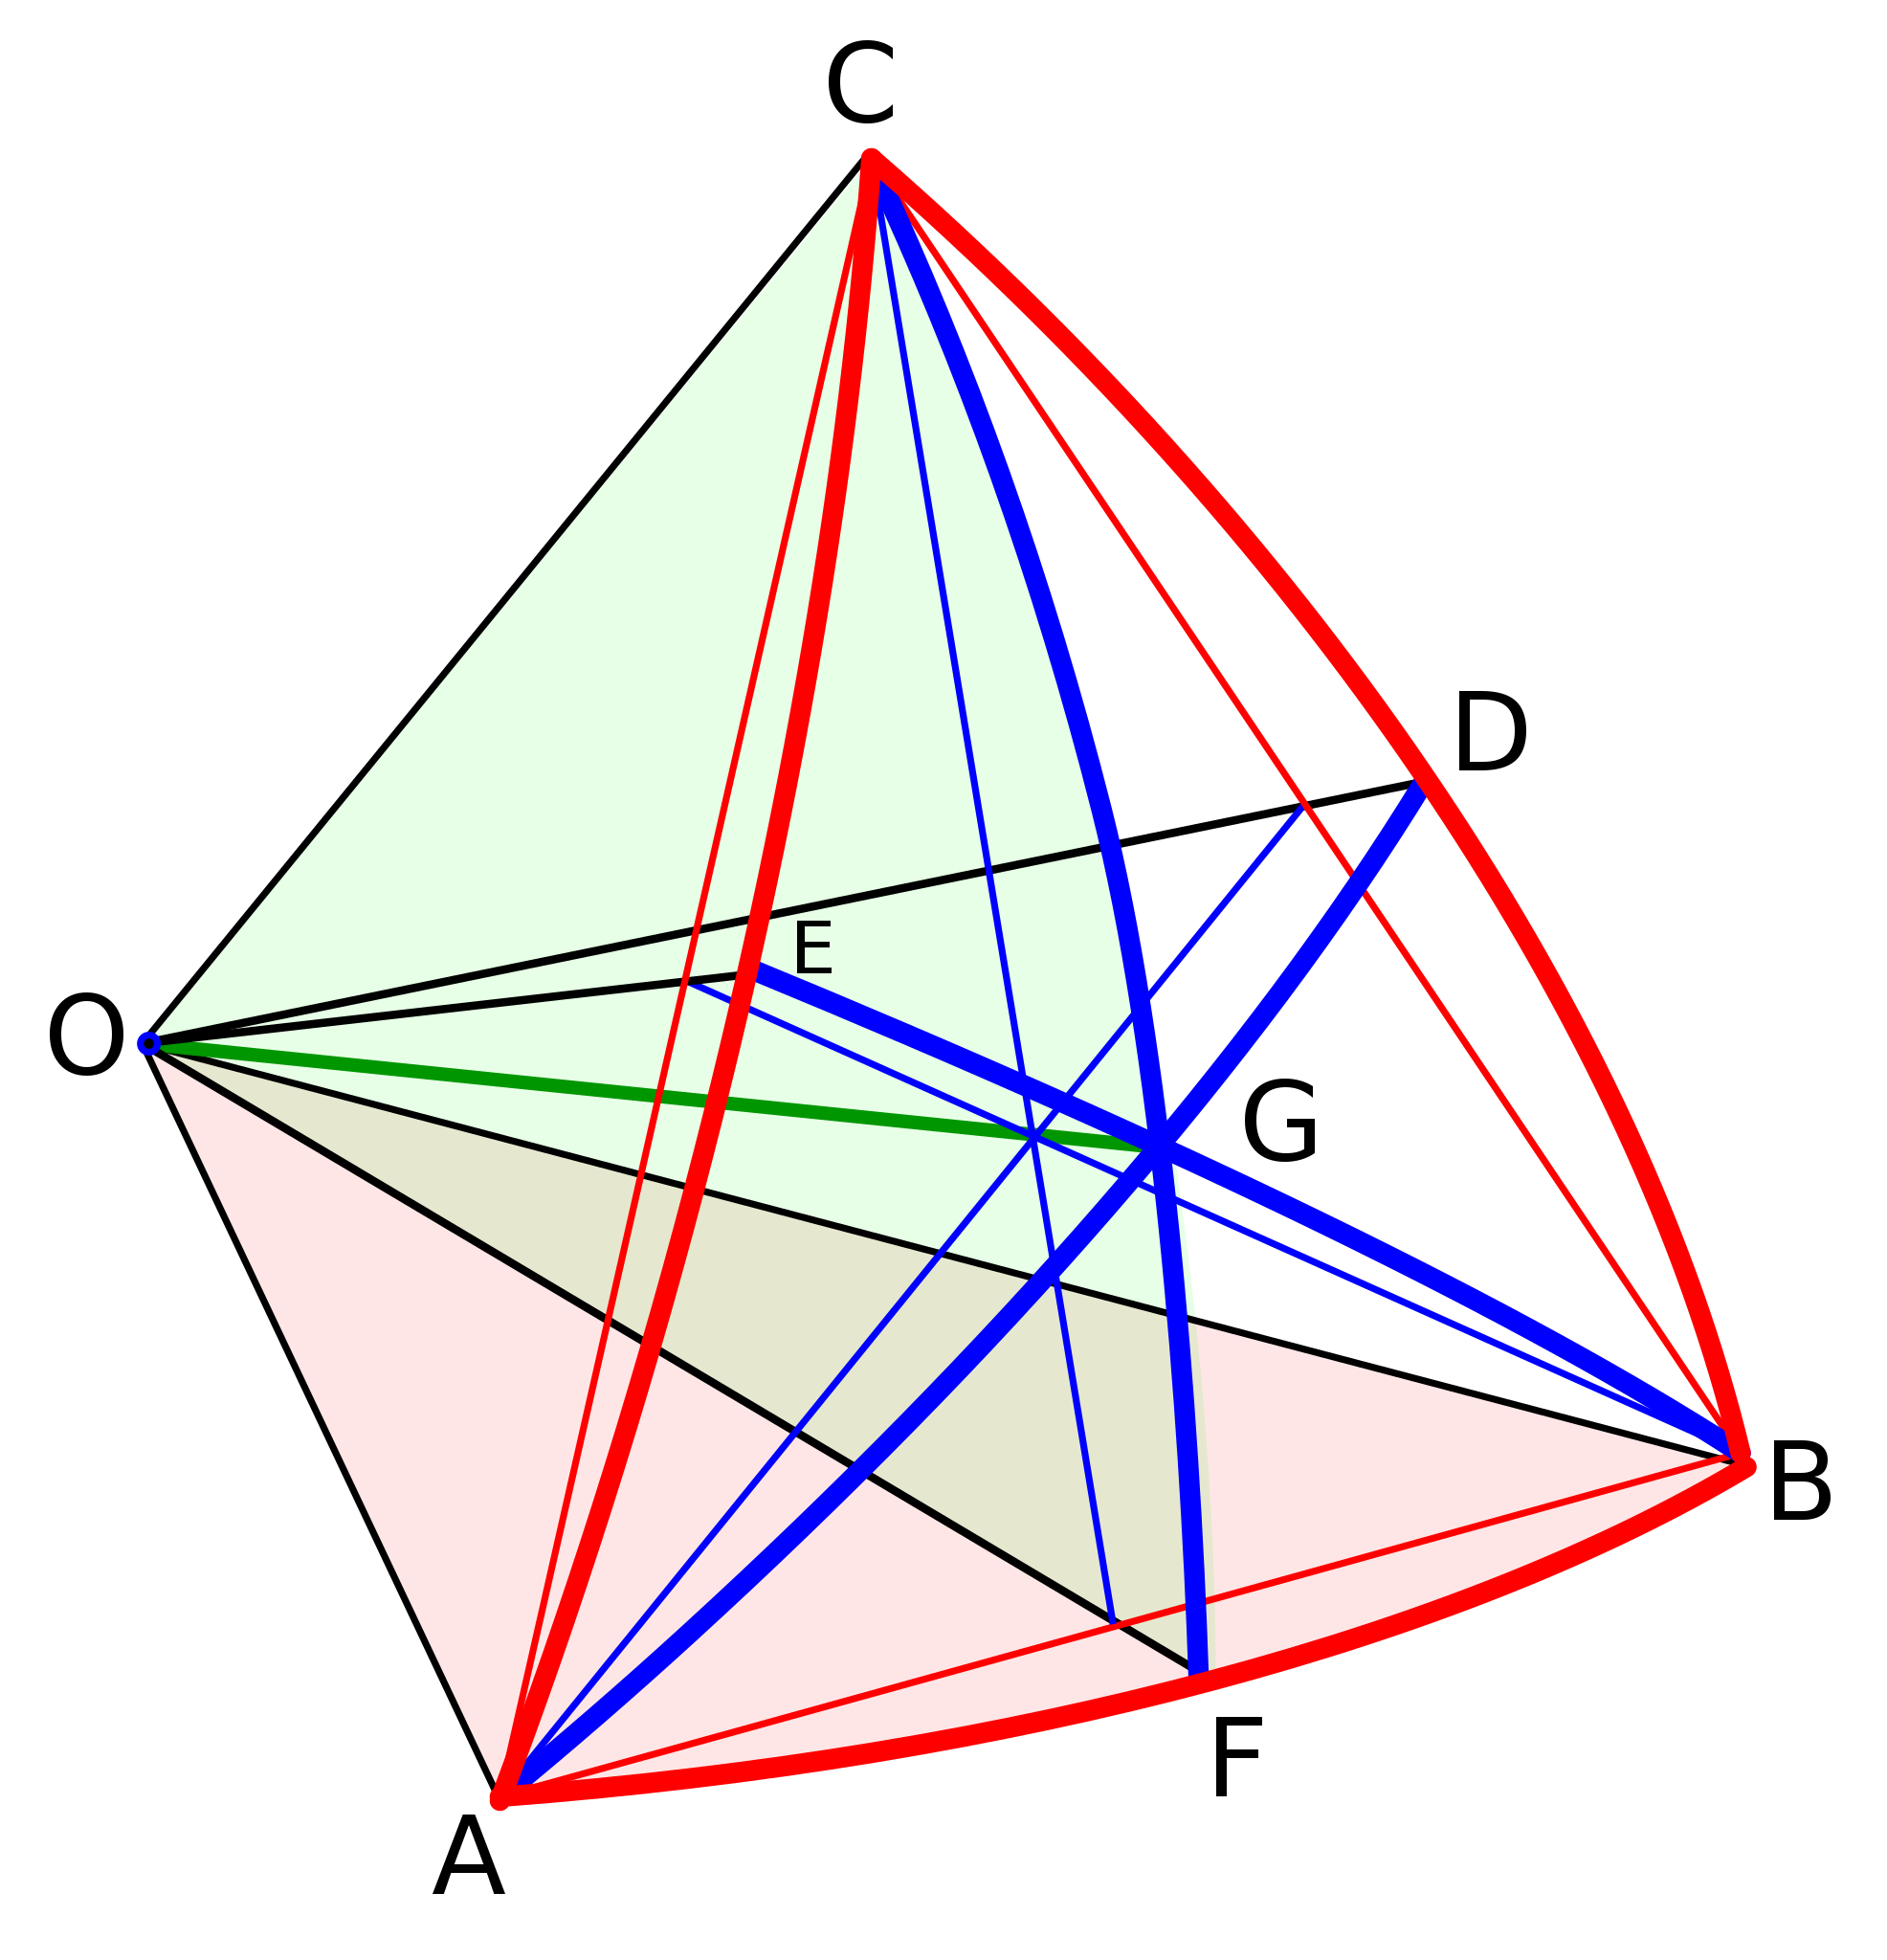
\includegraphics[width=0.4\textwidth]{IMG/Medians.png}
        \caption{Spherical Medians }
        \label{fig:medians}
    \end{figure}
    \begin{question}
        Let $O$ be the center of the sphere. If $G$ is the centroid of spherical triangle $ABC$ and $A'B'C'$ is the polar triangle of $ABC$, show that
        \begin{align*}
            {\overrightarrow {OG}}={\frac {1}{2E}}\cdot \left({\overrightarrow {OC'}}\cdot |{\overline {AB}}|+{\overrightarrow { OA'}}\cdot |{\overline {BC}}|+{\overrightarrow {OB'}}\cdot |{\overline {CA}}|\right).
        \end{align*}
    \end{question}
    \end{question}
\end{tcolorbox}



\subsection{63 Ancient Spherical Geometry Problems}

\begin{question}[name={1960 International Mathematical Olympiad}]
	% https://artofproblemsolving.com/community/c6h54832p341560
	Consider a cone of revolution with an inscribed sphere tangent to the base of the cone. A cylinder is circumscribed about this sphere so that one of its bases lies in the base of the cone. let $V_1$ be the volume of the cone and $V_2$ be the volume of the cylinder.
	\begin{tasks}
		\task Prove that $V_1 \neq V_2$;
		\task  Find the smallest number $k$ for which $V_1=kV_2$; for this case, construct the angle subtended by a diamter of the base of the cone at the vertex of the cone.
	\end{tasks}
\end{question}

\begin{solution}[name={Solution by Boxedexe}]
	Let $ O$, $ A$, $ B$, $ \theta$, and $ r$ be the cone's vertex, cone's base's center, a point on the cone's base's circle, $ \angle AOB$, and the radius of the sphere, respectively. Then it follows, from basic trigonometry, that $ OA = \frac {r(1 + \sin\theta)}{\sin\theta}$ and $ AB = \frac {r(1 + \sin\theta)}{\cos\theta}$. Hence, $$ V_1 = \frac {\pi AB^2OA}{3} = \frac {\pi\left(\frac {r(1 + \sin\theta)}{\cos\theta}\right)^2\left(\frac {r(1 + \sin\theta)}{\sin\theta}\right)}{3},$$ and $ V_2 = 2\pi r^3$. Ergo,
	\[ k = \frac {\pi\left(\frac {r(1 + \sin\theta)}{\cos\theta}\right)^2\left(\frac {r(1 + \sin\theta)}{\sin\theta}\right)}{6\pi r^3}\implies (1 + 6k)\sin^2\theta + (2 - 6k)\sin\theta + 1 = 0.
	\]
	However, the discriminant of the above quadratic equation must be non-negative, that is, $$ (1 - 3k)^2\geq 1 + 6k\implies k\geq\frac {4}{3},$$
	and the conclusion follows.
\end{solution}




\begin{question}[name={1962 International Mathematical Olympiad}]
	% https://artofproblemsolving.com/community/c6h55249p343382
	The tetrahedron $SABC$ has the following property: there exist five spheres, each tangent to the edges $SA, SB, SC, BC, CA, AB,$ or to their extensions.
	\begin{tasks}
		\task Prove that the tetrahedron $SABC$ is regular.
		\task Prove conversely that for every regular tetrahedron five such spheres exist.
	\end{tasks}
\end{question}

\begin{solution}
	This solution was written by \textbf{randomusername} on AoPS:
	\begin{tasks}
		\task Let $\mathcal{S}$ be the sphere tangent to the edges from the inside, and let $\mathcal{S}_X$ be the sphere tangent to the edges of the face opposite to vertex $X$, and the extensions of the edges from $X$.
		Consider say $\mathcal{S}$ and $\mathcal{S}_S$. If we cut these spheres by plane $ABC$, in both cases we get a circle on plane $ABC$ tangent to the segments $AB,BC,CA$ - this is the incircle of $\triangle ABC$. Hence $\mathcal{S}$ and $\mathcal{S}_S$ touches the edges $AB,BC,CA$ in the same points.
		Now cut the two spheres by plane $SAB$. We get the incircle and $S$-excircle of $\triangle SAB$. We have proven that $\mathcal{S}$ and $\mathcal{S}_S$ touch $AB$ in the same point, so the incircle and $S$-excircle of $\triangle SAB$ touch $AB$ at the same point. This implies that $SA=SB$.
		Similarly, we get that any two edges are the same length, therefore the tetrahedron is indeed regular.
		\task Look at the regular tetrahedron $SABC$.
		By symmetry, the center $O$ of the regular tetrahedron $SABC$ is of equal distance $d$ from all its edges, so taking $\mathcal{S}(O,d)$ works.
		Let the incenter of say $\triangle SAB$ be $I$, the $S$-excenter of $\triangle SAB$ be $J$. Consider the homothety with center $S$ that maps $I$ to $J$. This homothety maps the incircle $\omega$ of $\triangle SAB$ to the $S$-excircle of $\triangle SAB$; since $\omega\subset \mathcal{S}$, we have $\omega'\subset\mathcal{S}'$ and therefore $\mathcal{S}'$ also touches edge $AB$. By rotational symmetry, $\mathcal{S}'$ also touches edges $BC$ and $CA$. Moreover, because $\mathcal{S}$ touched edges $SA,SB,SC$, $\mathcal{S}'$ will touch the extensions of $SA,SB,SC$. This proves that $\mathcal{S}_S=\mathcal{S}'$ is up for the job.
		By symmetry, so do $\mathcal{S}_A,\mathcal{S}_B,\mathcal{S}_C$ exist.
	\end{tasks}
\end{solution}




\begin{question}[name={1966 International Mathematical Olympiad}]
	% https://artofproblemsolving.com/community/c6h56135p347440
	Prove that the sum of the distances of the vertices of a regular tetrahedron from the center of its circumscribed sphere is less than the sum of the distances of these vertices from any other point in space.
\end{question}


\begin{question}[name={1959--1966 IMO Longlist}]
	% https://artofproblemsolving.com/community/c6h16269p113444
	In a tetrahedron, all three pairs of opposite (skew) edges are mutually perpendicular. Prove that the midpoints of the six edges of the tetrahedron lie on one sphere.
\end{question}

\begin{solution}[name={Solution by Grobber}]
	This can basically be reduced to a plane geometry problem.
	
	The vertex $D$ is projected onto the orthocenter $H$ of $ABC$ (this follows from the conditions $AB\perp CD,\ AC\perp BD,\ AD\perp BC$). This means that the midpoints $U,V,T$ of $DA,DB,DC$ are projected onto the midpoints $X,Y,Z$ of $HA,HB,HC$. Let $M,N,P$ be the midpoints of $BC,CA,AB$. The points $M,N,P,X,Y,Z$ liue on the nine-point circle of $ABC$, so the points $U,V,T$ lie on a circle of radius equal to $\frac R2$ ($R$ is the circumradius of $ABC$) which lies on a plane parallel to $ABC$ and which has its center directly above the nine-point center of $ABC$. It's is now clear that $M,N,P,U,V,T$ lie on a sphere which has its center in the midpoint of the segment formed by the centers of $(MNP),(UVT)$.
\end{solution}




\begin{question}[name={1967 IMO Longlist}]
	% https://artofproblemsolving.com/community/c6h21133p137276
	Determine the volume of the body obtained by cutting the ball of radius $R$ by the trihedron with vertex in the center of that ball, it its dihedral angles are $\alpha, \beta, \gamma.$
\end{question}

\begin{solution}[name={Solution by Grobber}] 
	I remember solving this before the crash.\footnote{Written on December 16, 2004.}
	The ratio between this volume and the volume of the sphere is equal to the ratio between the area determined by the trihedron on the sphere and the area of the sphere. The region is a spherical triangle with angles $\alpha,\beta,\gamma$, and its area is thus $(\alpha+\beta+\gamma-\pi)\cdot R^2$. The volume we are looking for must then be $\frac{\alpha+\beta+\gamma-\pi}{4\pi}\cdot \frac{4\pi\cdot R^3}3=\frac{(\alpha+\beta+\gamma-\pi)\cdot R^3}3$.	
\end{solution}
	
	


\begin{question}[name={1967 IMO Longlist}]
	% https://artofproblemsolving.com/community/c6h21142p137298
	Prove this proposition: Center the sphere circumscribed around a tetrahedron which coincides with the center of a sphere inscribed in that tetrahedron if and only if the skew edges of the tetrahedron are equal.
\end{question}

\begin{solution}[name={Solution by Grobber}] 
	Let $ABCD$ be the tetrahedron. $I$, its incenter, is projected on the four planes of the faces in the circumcenters of the faces. Let $O_A,O_B,O_C,O_D$ be the circumcenters of $BCD$ and so on. We clearly have $d(O_D,BC)=d(O_A,BC)$, and therefore, $\angle BAC=\angle BDC$. From this equality and the like we find that the sum of the plane angles around each vertex is $\pi$ (call this assertion $(*)$). Now take the faces $BCD,CAD,ABD$ and rotate them around $BC,CA,AB$ until they are on the same plane as $ABC$. It is now easy to see from $(*)$ that $ABC,CBD,ADB,DAC$ are congruent, and the conclusion follows.
\end{solution}


\begin{question}[name={1970 Bulgaria}]
	% https://artofproblemsolving.com/community/c1068820h2598009p22411139
	In space, we are given the points $A,B,C$ and a sphere with center $O$ and radius $1$. Find the point $X$ from the sphere for which the sum $f(X)=|XA|^2+|XB|^2+|XC|^2$ attains its maximal and minimal value. Prove that if the segments $OA,OB,OC$ are pairwise perpendicular and $d$ is the distance from the center $O$ to the centroid of the triangle $ABC$ then:
	\begin{tasks}
		\task the maximum of $f(X)$ is equal to $9d^2+3+6d$;
		\task the minimum of $f(X)$ is equal to $9d^2+3-6d$.
	\end{tasks}
\end{question}	



\begin{question}[name={1979 USAMO}]
	% https://artofproblemsolving.com/community/c6h424758p2403729
	Let $S$ be a great circle with pole $P$. On any great circle through $P$, two points $A$ and $B$ are chosen equidistant from $P$. For any spherical triangle $ABC$ (the sides are great circles ares), where $C$ is on $S$, prove that the great circle are $CP$ is the angle bisector of angle $C$.
	
	\textbf{Note}: A great circle on a sphere is one whose center is the center of the sphere. A pole of the great circle $S$ is a point $P$ on the sphere such that the diameter through $P$ is perpendicular to the plane of $S$.
\end{question}

\begin{solution}[name={Solution by Luis González}] 
	% https://artofproblemsolving.com/community/c6h424758p2404678
	Reflection $C'$ of $C$ about $N$ also lies on the equator and since there are infinitely many great circles through $C,C'$, then we deduce that $C,C',A$ and $C,C',B$ lie on a great circle, respectively. $NC=NC',$ $NA=NB$ and $\sphericalangle ANC=\sphericalangle BNC'$ imply that the spherical triangles $ANC$ and $BNC'$ are congruent by SAS criterion. Therefore,  N-spherical altitudes of $ANC$ and $BNC'$ are congruent, i.e., $N$ is equidistant from the great circles $AC$ and $BC'$. Finally, $CN$ bisects the spherical lune formed by the great circles $CB$ and $CA$.
\end{solution}




\begin{question}[name={1981 USAMO}]
	% https://artofproblemsolving.com/community/c6h420408p2374672
	The sum of the measures of all the face angles of a given complex polyhedral angle is equal to the sum of all its dihedral angles. Prove that the polyhedral angle is a trihedral angle. \textbf{Note}: A convex polyhedral angle may be formed by drawing rays from an exterior point to all points of a convex polygon.
\end{question}

\begin{solution}[name={Solution from Kalva}] 
	Clearly, $n = 3$ is certainly possible. For example, take $\angle {APB} = \angle {APC} = \angle {BPC} = 90^{\circ}$ (so that the lines $PA, PB, PC$ are mutually perpendicular). Then the three planes through P are also mutually perpendicular, so the two sums are both $270^{\circ}$.
	
	We show that $n > 3$ is not possible.
	
	The sum of the n angles $APB$ etc at $P$ is less than $360^\circ$. This is almost obvious. Take another plane which meets the lines $PA, PB, PC$ etc at $A', B', C', \dots$ and so that the foot of the perpendicular from P to the plane lies inside the n-gon $A'B'C' \dots$ then as we move P down the perpendicular the angles $A'PB'$ etc all increase. But when it reaches the plane their sum is $360^\circ$. However, I do not immediately see how to make that rigorous. Instead, take any point $O$ inside the $n$-gon $ABC$. We have $\angle PBA + \angle PBC > \angle ABC$.
	
	Adding the n such equations we get $\sum(180^\circ - APB) > \sum ABC = (n - 2) 180^\circ$. So, $\sum APB < 360^\circ$.
	
	The sum of the n angles between the planes is at least $(n - 2)*180^o$. If we take a sphere center $P$. Then the lines $PA, PB$ intersect it at $A", B", \dots$ which form a spherical polygon. The angles of this polygon are the angles between the planes. We can divide the polygon into $n - 2$ triangles. The angles in a spherical triangle sum to at least $180^\circ$. So the angles in the spherical polygon are at least $(n - 2) 180^\circ$. So we have $(n - 2) 180^\circ < 360^\circ$ and hence $n < 4$.
\end{solution}




\begin{question}[name={1982 IMO Longlist}]
	% https://artofproblemsolving.com/community/c6h397013p2207949
	Let $r_1, \ldots , r_n$ be the radii of $n$ spheres. Call $S_1, S_2, \ldots , S_n$ the areas of the set of points of each sphere from which one cannot see any point of any other sphere. Prove that
	\[\frac{S_1}{r_1^2} + \frac{S_2}{r_2^2}+\cdots+\frac{S_n}{r_n^2} = 4 \pi.\]
\end{question}



\begin{question}[name={1982 IMO Longlist}]
	% https://artofproblemsolving.com/community/c6h397016p2207957
	A regular $n$-gonal truncated pyramid is circumscribed around a sphere. Denote the areas of the base and the lateral surfaces of the pyramid by $S_1, S_2$, and $S$, respectively. Let $\sigma$ be the area of the polygon whose vertices are the tangential points of the sphere and the lateral faces of the pyramid. Prove that
	\[\sigma S = 4S_1S_2 \cos^2 \frac{\pi}{n}.\]
\end{question}

\begin{solution}[name={Solution by Luis González}]
	Let $\mathcal{C}_1(r_1),\mathcal{C}_2(r_2)$, (with $r_2 >r_1$) are the incircles of the bases of the truncated pyramid. Let $\mathcal{C}_3(\varrho)$ be the circumcircle of the regular $n$--gon whose vertices are the tangency points of the subject sphere $\mathcal{E}$ with the lateral faces. Thus, $\mathcal{C}_1(r_1),\mathcal{C}_2(r_2)$ and $\mathcal{C}_3(\varrho)$ are obviously cross sections of a right cone with apex $A$ circumscribed around $\mathcal{E}.$ Arbitrary plane through the axis of the cone cuts $\mathcal{E}$ into a circle $(I)$ and the bases $\mathcal{C}_2(r_2),\mathcal{C}_1(r_1) ,$ into the segments $BC=2r_2,$ $MN=2r_1,$ $(M \in AB$ and $N \in AC)$ $\Longrightarrow$ $BCNM$ is an isosceles trapezoid with incircle $(I).$ If $(I)$ touches $AB,AC$ at $D,E,$ then $DE=2\varrho, $ $NE=r_1$ and $CE=r_2.$ Therefore
	\[DE=\frac{BC \cdot EN+MN \cdot EC}{NC},\]
	so that \[\varrho= \frac{2r_1r_2}{r_1+r_2} \ (\star).\]
	
	From the well-known formulae of the areas of regular polygons, we have:
	$$\sigma=n\varrho^2\cos \frac{\pi}{n}\sin \frac{\pi}{n},$$
	and also
	$$S_1=n \cdot {r_1}^2\tan \frac{\pi}{n} \qquad \text{and} \qquad S_2=n \cdot {r_2}^2 \tan \frac{\pi}{2},$$
	which results in $$S_1S_2=n^2 {r_1}^2 {r_2}^2 \tan^2 \frac{\pi}{n}.$$
	
	Lateral faces of the truncated pyramid are congruent isosceles trapezoids with altitude $r_1+r_2,$ whose bases are the sides of the $n$--gons with incircles $\mathcal{C}_1(r_1),\mathcal{C}_2(r_2).$ Therefore,
	$$S=\frac{n}{2} \cdot (r_1+r_2) \cdot \left(2 r_1 \tan \frac{\pi}{n}+2 r_2 \tan \frac{\pi}{n} \right )=n(r_1+r_2)^2 \tan \frac{\pi}{n}.$$
	Substituting $\varrho, r_1r_2$ and $(r_1+r_2)$ from the latter expressions into $(\star)$ yields:
	$$\frac{\sigma}{n \cos \frac{\pi}{n} \sin \frac{\pi}{n}}=\frac{4S_1 S_2}{n^2 \tan^2 \frac{\pi}{n}} \cdot  \frac{n \tan \frac{\pi}{n}}{S} \Longrightarrow \ \sigma  S=4 S_1 S_2 \cos^2 \frac{\pi}{n}.$$
\end{solution}


\begin{question}[name={1983 IMO Longlist}]
	% https://artofproblemsolving.com/community/c6h370533p2041537
	Four faces of tetrahedron $ABCD$ are congruent triangles whose angles form an arithmetic progression. If the lengths of the sides of the triangles are $a < b < c$, determine the radius of the sphere circumscribed about the tetrahedron as a function on $a, b$, and $c$. What is the ratio $c/a$ if $R = a$?
\end{question}


\begin{question}[name={1984 IMO Longlist}]
	% https://artofproblemsolving.com/community/c6h371118p2046259
	A tetrahedron is inscribed in a sphere of radius $1$ such that the center of the sphere is inside the tetrahedron. Prove that the sum of lengths of all edges of the tetrahedron is greater than $6$.
\end{question}



\begin{question}[name={1985 IMO Longlist}]
	% https://artofproblemsolving.com/community/c6h366736p2018314
	This problem comes in two parts:
	\begin{tasks}
		\task The solid $S$ is defined as the intersection of the six spheres with the six edges of a regular tetrahedron $T$, with edge length $1$, as diameters. Prove that $S$ contains two points at a distance $1/\sqrt 6$.
		\task Using the same assumptions in a), prove that no pair of points in $S$ has a distance larger than $1/\sqrt 6$.
	\end{tasks}
\end{question}




\begin{question}[name={1985 IMO Longlist}]
	% https://artofproblemsolving.com/community/c6h364221p2000927
	Determine the radius of a sphere $S$ that passes through the centroids of each face of a given tetrahedron $T$ inscribed in a unit sphere with center $O$. Also, determine the distance from $O$ to the center of $S$ as a function of the edges of $T$.
\end{question}

\begin{solution}[name={Solution by Luis González}]
	For the sake of generality, let $\mathcal{O} \equiv (O,R)$ be the circumsphere of the tetrahedron $ABCD$ and $ \mathcal{S} \equiv (S,R')$ be the circumsphere of the tetrahedron whose vertices are the centroids $A',$ $B',$ $C',$ $D'$ of its faces against $A,B,C,D.$ Segments $AA',$ $ BB',$ $ CC',$ $ CC',$ $DD'$ concur at the centroid $G$ of $ABCD,$ such that $G$ divides them in the same ratio $1:3$, therefore, Tetrahedra $A'B'C'D'$ and $ABCD$ are homothetic through the homothety with center $G$ and coefficient $-\frac{_1}{^3}.$ Therefore, $R'=R/3$ and $OS=4OG/3.$ Let $a,b,c,d,e,f$ be the edges of $ABCD.$ By Leibniz theorem for the circumcenter $O$ of $ABCD,$ we have
	\begin{align*}
		OG^2 &= \frac{OA^2+OB^2+OC^2+OD^2}{4}-\frac{a^2+b^2+c^2+d^2+e^2+f^2}{16}\\
		&= R^2-\frac{a^2+b^2+c^2+d^2+e^2+f^2}{16},
	\end{align*}
	and finally,
	\[ OS^2=\frac{16R^2}{9}-\frac{a^2+b^2+c^2+d^2+e^2+f^2}{9}.\]
\end{solution}



\begin{question}[name={1987 IMO Longlist}]
	% https://artofproblemsolving.com/community/c6h362762p1989386
	Let $S_1$ and $S_2$ be two spheres with distinct radii that touch externally. The spheres lie inside a cone $C$, and each sphere touches the cone in a full circle. Inside the cone there are $n$ additional solid spheres arranged in a ring in such a way that each solid sphere touches the cone $C$, both of the spheres $S_1$ and $S_2$ externally, as well as the two neighboring solid spheres. What are the possible values of $n$?
\end{question}


\begin{solution}[name={Solution by Spanferkel}]
	% https://artofproblemsolving.com/community/c6h362762p2493035
	Let the radii of $S_1$ and $S_2$ be $a>b$. Then by considering a plane through the axis of the cone that intersects one of the solid spheres, say $S_3$, in a maximal circle, we get by Descartes' theorem for the radius $r$ of $S_3$:
	$$\frac1{\sqrt{r}}=\frac1{\sqrt{a}}+\frac1{\sqrt{b}},$$ or $$r=\frac{ab}{(\sqrt{a}+\sqrt{b})^2}.$$
	For the (half) opening angle $\phi$ of the cone, we have $$\sin\phi=\frac{a-b}{a+b}.$$ Define $\psi$ by $$\sin\psi=\frac{b-r}{b+r},$$ (this is the corresponding angle intervening between $S_2$ and $S_3$).
	
	Let $R$ denote the distance of the center of $S_3$ from the axis of the cone. Then we have
	\begin{align*}
		R &= (b+r)\sin(\phi+\psi)\\
		&=2\frac{(a-b)\sqrt{br}+(b-r)\sqrt{ab}}{a+b} \\
		&=\frac{2ab(a+b+\sqrt{ab})}{(a+b)(\sqrt{a}+\sqrt{b})^2}.
	\end{align*}
	So, $$\frac rR=\frac{a+b}{2(a+b+\sqrt{ab})}=\frac{1}{2+\frac{2\sqrt{x}}{1+x}},$$ where $x=b/a$. This function is decreasing in $(0,1)$ with values between $\frac12$ and $\frac13$. As we want $$\frac rR=\sin\frac\pi n,$$ we get $n=7,8,9$. The limit case $n=6$ (for $x\to 0$) cannot be attained.
\end{solution}




\begin{question}[name={1987 Vietnam}]
	% https://artofproblemsolving.com/community/c6h255546p1395616
	Prove that among any five distinct rays $ Ox$, $ Oy$, $ Oz$, $ Ot$, $ Or$ in space there exist two which form an angle less than or equal to $ 90^{\circ}$.
\end{question}

\begin{solution}[name={Solution by Mij}] 
	% https://artofproblemsolving.com/community/c6h255546p1401160
	We assume for the sake of contradiction that all angles determined by any two of the five rays are greater than $ 90^\circ$.
	
	Consider a sphere centered at $ O$, and let $ Ox,Oy,Oz,Ot,Or$ intersect the sphere at $ x, y, z, t, r$ respectively.
	The plane perpendicular to $ Ox$ at $ O$ cuts the sphere into two hemispheres.
	Let $ A$ be the hemisphere containing $ x$. $ y$ cannot lie on $ A$, because if it did, the angle $ \angle xOy$ would be less than or equal to $ 90^\circ$.
	By the same argument $ z, t, r$ cannot lie on $ A$. Define hemispheres $ B$, $ C$, $ D$, and $ E$ similarly, to contain $ y, z, t, r$, respectively and have similar properties.
	
	Each of the five hemispheres has a measure of $ 2 \pi$ radians. Because of the assumption, any two hemispheres must overlap at a solid angle of less than $ \pi$ radians. Let the intersection of $ A$ and $ B$ have measure $ \theta < \pi$.
	The union of $ A$ and $ B$ must have measure $ 2\pi + 2\pi - \theta = 4\pi - \theta$, and a complement $ G$ of measure $ 4\pi - (4\pi - \theta) = \theta$, and be bounded by two semi-great-circles that meet at two points, $ p$ and $ q$. The complement $ G$ is contained within what it would be if its measure were its upper bound of $ \pi$.
	
	The intersection of $ G$ and $ C$ has a minimum of $ \dfrac{\theta}{2}$ as $ z$ approaches either $ p$ or $ q$, so it is greater than $ \dfrac{\theta}{2}$. Thus the union of $ A, B, C$ has measure greater than 
	$$ (4\pi - \theta) + \dfrac{\theta}{2} = 4\pi - \dfrac{\theta}{2},$$ so the complement $ H$ of this union has measure less than $\theta/2 < \pi/2$, and is contained within what it would be if $ z$ were at $ p$ or $ q$.
	
	Finally, $ H$ is contained within what it would be if $ z$ were at $ p$ or $ q$ and, since $ H$ is a subset of $ G$, within what $ H$ would be if $ \theta$ equals $ \pi$. This would be a $ 90^\circ$-$ 90^\circ$-$ 90^\circ$ spherical triangle, so $ H$ is a subset of a $ 90^\circ$--$ 90^\circ$--$ 90^\circ$ spherical triangle. Since $ t$ and $ r$ must lie on $ H$, and therefore a $ 90^\circ$--$ 90^\circ$--$ 90^\circ$ spherical triangle, $ \angle tOr \le 90^\circ$. We have contradicted our assumption, so we are done.
\end{solution}



\begin{question}[name={1992 Putnam}]
	% https://artofproblemsolving.com/community/c6h538673p3097350
	On a sphere, $4$ points are randomly chosen. What is the probability that the center of the sphere is contained in the tetrahedron in the $4$ points.
\end{question}

\begin{solution}[name={Solution by Dinoboy}]
	% https://artofproblemsolving.com/community/c6h538673p3097505
	Consider three points $A,B,C$ on a sphere and for a point $X$ denote $X'$ is reflection across the center of the sphere. Then note that a point $D$ satisfies the center of the sphere is in tetrahedron $ABCD$ if and only if $D$ lies in the spherical section bounded by the arcs $A'B', A'C', B'C'$ (let's just call this triangle $A'B'C'$ for simplicity). Thus the problem reduces to finding the expected area of a triangle on a sphere of area $1$. But note that every point of the sphere is in exactly one of $XYZ$ for $X \in \{A,A'\}, Y \in \{B,B'\}, Z \in \{C,C'\}$ so it follows the sum of those triangle's areas is $1$. Then since we have established each triangle can be uniquely paired with 7 other triangles, it immediately follows the expected area is $1/8$, so we are done.
\end{solution}



\begin{question}[name={2006 Baltic Way}]
	% https://artofproblemsolving.com/community/c6h233736p1290840
	% Official solutions: https://www.balticway07.dk/data/ekstra/bw02-06-online-a5.pdf
	There are $2006$ points marked on the surface of a sphere. Prove that the surface can be partitioned into $2006$ congruent pieces, so that each piece contains exactly one of these points inside it.
\end{question}


\begin{question}[name={2016 Brazil Cono Sur Training}]
	% https://artofproblemsolving.com/community/c1068820h2714197p23600514
	Let $ABCD$ be a tetrahedron and let $E$, $F$, $G$, $H$, $K$, and $L$ be points on the segments $AB$, $BC$, $CA$, $DA$, $DB$ and $DC$, respectively, so that $$AE \cdot BE = BF\cdot  CF = CG \cdot  AG = DH \cdot  AH = DK \cdot  BK = DL \cdot  CL.$$ Prove that the six points marked on the sides of the tetrahedron are on the same sphere.
\end{question}


\begin{question}[name={2000 Belarus TST}]
	% https://artofproblemsolving.com/community/c1068820h2007371p14054432
	A closed pentagonal line is inscribed in a sphere of the diameter $1$, and has all edges of length $\ell$.
	Prove that $$\ell \le  \sin \frac{2\pi}{5}.$$
\end{question}



\begin{question}[name={1995 Romania TST}]
	% https://artofproblemsolving.com/community/c1068820h2009035p14075310
	A cube is partitioned into finitely many rectangular parallelepipeds with the edges parallel to the edges of the cube. Prove that if the sum of the volumes of the circumspheres of these parallelepipeds equals the volume of the circumscribed sphere of the cube, then all the parallelepipeds are cubes.
\end{question}


\begin{question}[name={1998 Czech and Slovak}]
	% https://artofproblemsolving.com/community/c1068820h2011826p14103553
	A sphere is inscribed in a tetrahedron $ABCD$. The tangent planes to the sphere parallel to the faces of the tetrahedron cut off four smaller tetrahedra. Prove that sum of all the $24$ edges of the smaller tetrahedra equals twice the sum of edges of the tetrahedron $ABCD$.
\end{question}




\begin{question}[name={1993 Brazil}]
	% https://artofproblemsolving.com/community/c6h570480p3350098
	Let $P_1P_2 \dots P_n$ a polygon inscribed on a circunference and contained in a plane $\alpha$. Let $Q$ be a point outside $\alpha$. Consider, for each $i=1,2, \dots ,n$, the plane $\beta_i$ passing through $P_i$ and perpendicular to $QP_i$. Prove that all the planes $\beta_i$ intersect at one point.
\end{question}




\begin{question}[name={2015 Kurchatov Olympiad}]
	% https://artofproblemsolving.com/community/c6h2479315p20801553
	To prepare mashed potatoes, Kolya, the chef, needs to get the specified amount of peeled potatoes as soon as possible. Not caring about saving peelings, he cuts cubes from spherical potatoes, with each stroke clearing one edge of the knife. Can he complete the task faster when the same frequency of knife strokes if you cut out any other polyhedra? (formally: is it true that of all polyhedra cut from of the given sphere, the largest ratio of volume to the number of faces is for the inscribed cube?)
\end{question}





\begin{question}[name={2015 Miklos Schweitzer}]
	% https://artofproblemsolving.com/community/c6h1220043p6095752
	We call a bar of width ${w}$ on the surface of the unit sphere ${\Bbb{S}^2}$, a spherical segment, centered at the origin, which has width ${w}$ and is symmetric with respect to the origin.
	Prove that there exists a constant ${c>0}$, such that for any positive integer ${n}$ the surface ${\Bbb{S}^2}$ can be covered with ${n}$ bars of the same width so that any point is contained in no more than ${c\sqrt{n}}$ bars.
\end{question}




\begin{question}[name={2017 St. Petersburg}]
	% https://artofproblemsolving.com/community/c6h1637659p10305285
	Given a tetrahedron $PABC$, draw the height $PH$ from vertex $P$ to $ABC$. From point $H$, draw perpendiculars $HA’,HB’,HC’$ to the lines $PA,PB,PC$. Suppose the planes $ABC$ and $A’B’C’$ intersects at line $\ell$. Let $O$ be the circumcenter of triangle $ABC$. Prove that $OH\perp \ell$.
\end{question}





\begin{question}[name={2018 Spain}]
	% https://artofproblemsolving.com/community/c6h1609983p10050519
	Points on a spherical surface with radius $4$ are colored in $4$ different colors. Prove that there exist two points with the same color such that the distance between them is either $4\sqrt{3}$ or $2\sqrt{6}$ (distance is Euclidean, that is, the length of the straight segment between the points).
\end{question}



\begin{question}
	% https://artofproblemsolving.com/community/c6h264204p1434371
	Given reals $ a_i ,b_i,c_i$, for $ i=1,2,\dots,n$, such that \[\sum_{i=1}^n a_{i}^2=1, \qquad  \sum_{i=1}^n b_{i}^2=1, \qquad \sum_{i=1}^n c_{i}^2=1, \qquad \sum_{i=1}^n b_ic_i=0.\]
	Prove that $$\left(\sum_{i=1}^n a_ib_i\right)^2+\left(\sum_{i=1}^n a_ic_i\right)^2 \leq 1.$$
\end{question}



\begin{solution}[name={Solution by Spanferkel and Arqady}] 
	% https://artofproblemsolving.com/community/c6h264204p1711143
	Generally, for vectors $ \vec a, \vec b, \vec c\in\mathbb R^n$, we can write the ``spherical triangle inequality'' $ \alpha + \beta\ge \gamma$, as
	\[ \cos^2\alpha + \cos^2\beta + \cos^2\gamma\le1 + 2\cos\alpha\cos\beta \cos\gamma.\]
	Equivalently
	\[ \sum\frac { (\vec a\cdot\vec b)^2}{\vec a^2\vec b^2}\le1 + 2\frac {(\vec a\cdot\vec b) (\vec b\cdot\vec c) (\vec c\cdot\vec a)}{\vec a^2\vec b^2\vec c^2},\]
	or
	\[ \sum { {\vec c^2}(\vec a\cdot\vec b)^2}\le \vec a^2\vec b^2\vec c^2 + 2(\vec a\cdot\vec b) (\vec b\cdot\vec c) (\vec c\cdot\vec a).\]
\end{solution}



\begin{question}[name={Spherical Inequality by Puuhikki}]
	% https://artofproblemsolving.com/community/c6h114290p649085
	Let $x,y,z$ be positive real numbers such that $x^{2}+y^{2}+z^{2}=1$. Prove that \[8xyz<\frac{4}{3}\pi.\]
\end{question}


\begin{solution}[name={Solution by Arne}] 
	Consider a box inscribed in the sphere with equation $x^{2}+y^{2}+z^{2}= 1$, such that the coordinates of its vertices are $\left(\pm x, \pm y, \pm z\right)$. The volume of the box is $8xyz$. Of course the volume of the box is strictly smaller than the volume of the sphere, which is $4\pi/3$.
\end{solution}




\begin{question}[name={2002 Iran TST}]
	% https://artofproblemsolving.com/community/c6h5060p16012
	There is a closed curve on the surface of the unit sphere. We know every big circle of the sphere has non-empty intersection with the curve. Prove that perimeter of the curve is at least $2 \pi$.
\end{question}


\begin{solution}[name={Solution by Fedor Petrov}] 
	% https://artofproblemsolving.com/community/c6h5060p1080266
	The idea of possible geometric solution is that if any four points of our curve lie in the same half-space, then the whole curve also does. (Boundary of half-space contains the centre of a sphere). It follows from Helly theorem. Then we just need to prove that if $A$, $B$, $C$, and $D$ are four points on a sphere such that $O$ lies inside $ABCD$, then the perimetr of $A-B-C-D-A$ is at least $ 2\pi$. Let $D'$ be opposite of $D$, then $ D'$ lies inside spherical triangle $ABC$, so we have $AD'+CD'<AB+BC$ (the proof is as on the plane). But, \[AD+DC=2\pi-(AD'+CD'),\] so it's exactly what we need.
\end{solution}




\begin{question}[name={2003 China}]
	% https://artofproblemsolving.com/community/c6h202198p1111937
	$8$ spherical balls of radius $1$ are placed in a cylinder in two layers. with each layer containing $4$ balls. Each ball is tangent to $2$ balls in the same layer, $2$ balls in another layer, one base, and the lateral surface of the cylinder. What is the height of the cylinder?
\end{question}


\begin{solution}
	The problem reduces to solving $\sqrt{(\sqrt{2}-1)^2+1^2+(z-1)^2} = 2$ for $z$. The answer is $2+\sqrt[4]{8}$.
\end{solution}



	
\begin{question}
	On a circle of positive integer radius $n$, there are $m$ chords such that for any point in the circle there is a chord such that the distance from that point to the chord is $\leq 1$. Prove that $m \geq n$.
\end{question}


\begin{solution}[name={Solution by Grobber}] 
	% https://artofproblemsolving.com/community/c6h33912p210445
	This idea is on the verge of becoming too old, unfortunately...\footnote{Written on April 17, 2005}
	
	Consider the circle as the projection of a sphere of radius $n$ on the plane, and in this sphere, consider some spherical segments which are projected onto bands in our circle, each band being contained between two parallel lines, each line a distance $1$ from one of our chords.
	
	The hypothesis tells us that the segments cover the sphere (the area of the sphere), so the sum of their areas must be at least $4\pi n^2$. However, the lateral area of a segment with height $h$ is $2\pi nh$, and since all our segments have height $\le 2$, we get the desired conclusion.
\end{solution}



\begin{question}
	Four distinct points $A, B, C$, and $M$ are given on a sphere, none of which is opposite to any other. Prove that if the great circles $AM$ and $BM$ are orthogonal to great circles $BC$ and $AC$, respectively, then also the great circle $CM$ is orthogonal to great circle $AB$.
\end{question}


\begin{solution}[name={Solution by Grobber}] 
	% https://artofproblemsolving.com/community/c6h75136p432874
	In other words, the altitudes are concurrent in a spherical triangle.
	
	Let $O$ be the center of the sphere. We know that $OM$ is contained in the unique plane through $OA$ orthogonal to $(OBC)$, and also in the unique plane through $OB$ orthogonal to $(OCA)$, and we want to prove that it is also contained in the plane through $OC$ which is orthogonal to $(OAB)$. The problem is now this:
	
	Let $\alpha,\beta,\gamma$ be three planes through a point $O$, and let $a=\beta\cap\gamma,b=\gamma\cap\alpha,c=\alpha\cap\beta$. Prove that the planes $\pi_\alpha,\pi_\beta,\pi_\gamma$, passing through $a,b,c$ and orthogonal to $\alpha,\beta,\gamma$ respectively, share a point different from $O$ (in other words, they share a line).
	
	Pick $A\in a$, and then $B\in b,C\in c$ such that $AB\perp c,AC\perp b$. It's easy to see that $BC\perp a$ (you can prove this just like you prove the concurrence of the altitudes in a triangle by using scalar products), which means that $\pi_\alpha,\pi_\beta,\pi_\gamma$ cut the triangle $ABC$ along its altitudes. Since they are concurrent, the concurrence point is a point different from $O$ belonging to all $\pi$'s.
\end{solution}





\begin{question}[name={1992 Tokyo University Entrance Exam}]
	% https://artofproblemsolving.com/community/c6h21376p138342
	Let $a$ and $b$ be positive reals. Four points $P(0,0,0),Q(a,0,0),R(0,1,0),S(0,1,b)$ lie on a same spherical surface with radius $1$. Let $r$ be the radius of the sphere which is inscribed in tetrahedron $PQRS$. Find the maximum value of $r$.
\end{question}



\begin{question}[name={1993 Kyoto University Entrance Exam}]
	% https://artofproblemsolving.com/community/c6h21829p140733
	Assume that $3$ Points $A,B,C$ lie on the spherical surface with radius $1$, centered at $O$. Let $P,Q,R$ be the mid points of $BC,CA,AB$, respectively. Prove that at least one segment of the segments $OP,OQ,OR$ in length is greater than or equal to $\frac{1}{2}$.
\end{question}



\begin{solution}[name={Solution by Grobber}] 
	Well, since $\angle BOC+\angle COA+\angle AOB\le 2\pi$, we get that at least one of them is $\le 120^{\circ}$, and that's pretty much it.
\end{solution}




\begin{question}[name={1999 Australian Math Competition}]
	% https://artofproblemsolving.com/community/c6h39446p246212
	When three spherical balls, each of radius 10 cm, are placed in a hemispherical dish, it is noticed that the tops of the balls are all exactly level with the top of the dish. What is the radius, in centimeters, of the dish?
\end{question}



\begin{solution}[name={Solution by Yetti}] 
	Let $A, B, C$ be the centers of the 3 congruent spherical balls $(A), (B), (C)$, touching each other and forming an equilateral triangle with the side $AB = 2r = 20\ \text{cm}$. Let $H$ be the orthocenter of this equilateral triangle. Let $D$ be the center of the sphere $(D)$ of the hemispherical dish centered in the common tangent plane of the spheres $(A), (B), (C)$. The distance of the center $A$ from the vertical axis $DH$ of the hemispherical dish is equal to \[AH = AB \frac{\sqrt 3}{3} = \frac{2r \sqrt 3}{3}.\]
	Using Pythagorean theorem for the right angle triangle $\triangle AHD$,
	\[DA = \sqrt{DH^2 + AH^2} = \sqrt{r^2 + \frac{4r^2}{3}} = r \sqrt{\frac 7 3}.\]
	The tangency point $T$ of the spheres $(A)$ and  $(D)$ is on their center line $DA$ and the radius of the sphere $(D)$ is
	\begin{align*}
		R = DT &= DA + AT = r \sqrt{\frac 7 3} + r \\ 
		&= \left(1 + \sqrt{\frac 7 3}\right) r \doteq 2.5275\ r \\
		&= 25. 275\ \text{cm}.
	\end{align*}
\end{solution}




\begin{question}[name={1981 IMO Shortlist and Beyond}]
	% https://artofproblemsolving.com/community/c6h1465p4678
	The version b) is an ISL problem from 1981. The version a) is the easier 2-dimensional counterpart of the 3-dimensional version b).
	\begin{tasks}
		\task If a circular planet lies completely within the convex hull $H$ of a similarly defined system of circular planets, its entire circumference is visible from the other planets.
		\task Consider a cluster of n spherical planets, all the same size, which drift rigidly together through outer space, that is, each with no motion relative to the others in the cluster. In general, there is some region R on the surface of a planet which cannot be seen from any point on any of the other planets (if a planet is in the midst of the others, then its surface is completely visible and this region is empty). Prove that the sum of the areas of these visible regions R is exactly equal to the area of the surface of one planet.
	\end{tasks}
\end{question}



\begin{solution}[name={Solution by Grobber}] 
	% https://artofproblemsolving.com/community/c6h1465p9084
	I think (a) isn't that hard (not even the 3D version).
	
	Let's assume a certain point from the circumference of the planet isn't visible from any point from any of the other planets. We draw the tangent to the circle at that particular point. The semi--plane defined by this tangent, which doesn't contain the circle, can't contain any points from any circles, because otherwise the point would be visible, but this means that the point is on the convex hull, and not inside it, which ends the proof.
	
	We do the same in the case of spheres, by drawing the plane which is tangent to the sphere at the point which we want to show is invisible.
	
	This only defines the set of points which are invisible from any other points: those points which are ON the convex hull, and not INSIDE it. Proving that this region has an area equal to that of each of the spheres is another problem... 
	
	An observation: for each sphere which has invisible points, the region which is invisible is a polygon on the sphere; by this I mean a polygon on the sphere, which has arcs of large circles of the sphere as its ``sides.''
\end{solution}






\begin{question}[name={Problem 2814 in Gazeta Matematica (Bucuresti)}]
	% https://artofproblemsolving.com/community/c6h69121p405934
	Let $A',B',C'$ be the points where the arc bisectors of the spherical triangle $ABC$ meet the opposite sides. Is it possible to have $A'B'=A'C'$ without $ABC$ being an isosceles triangle?
\end{question}




\begin{question}
	% https://artofproblemsolving.com/community/c6h68171p406851
	Prove that the following two statements are equivalent, and then prove them separately.
	\begin{tasks}
		\task  For $a,b,c \geq 0$ satisfying $a^2+b^2+c^2=1$, we have
		\[\frac{a}{a^3+2bc}+\frac{b}{b^3+2ca}+\frac{c}{c^3+2ab} \geq 2.\]
		\task Using spherical coordinates, where $\alpha$ is the $x-y$ angle, and $\beta$ is the $y-z$ angle, define $a = \cos \beta \cos \alpha$ (x-coordinate), $b = \cos \beta \sin \alpha$ (y-coordinate), and finally $c = \sin \beta$. Then, we have \begin{multline*}
			\frac{\cos \alpha}{\cos^2 \beta \cos^3 \alpha + 2 \sin \beta \sin \alpha} + \frac{\sin \alpha}{\cos^2 \beta \sin^3 \alpha + 2 \sin \beta \cos \alpha}\\ + \frac{\sin \beta}{\sin^3 \beta + 2 \sin \alpha \cos \alpha \cos^2 \beta}  \geq 2.
		\end{multline*}
	\end{tasks} 
\end{question}




\begin{question}[name={Cauchy--like Spherical Inequality by Fuzzylogic}]
	% https://artofproblemsolving.com/community/c6h81833p468969
	Let $a_i,b_i,x_i$ be reals for $i=1,2,\dots,n$, such that $\sum_{i=1}^na_ix_i=0$. Prove that
	\[ \bigg(\sum_{i=1}^n x_i^2\bigg) \bigg(\sum_{i=1}^na_i^2\sum_{i=1}^nb_i^2 - \big(\sum_{i=1}^na_ib_i\big)^2\bigg) \ge \bigg(\sum_{i=1}^na_i^2\bigg)\bigg(\sum_{i=1}^nb_ix_i\bigg)^2.  \]
\end{question}





\begin{solution}[name={Solution by Spanferkel}] 
	% https://artofproblemsolving.com/community/c6h81833p469030
	Here is a geometrical proof. Let $a,b,c\in\mathbb{R}^n$ be the corresponding vectors. Then we can write the inequality as
	\[x^2(a^2b^2- \langle a,b \rangle ^2)\ge a^2 \langle b,x \rangle ^2.\]
	This inequality is equivalent to
	\[ 1\ge\frac{ \langle b,x \rangle ^2}{b^2x^2}+\frac{ \langle a,b \rangle ^2}{a^2b^2}=\cos^2(b,x)+\cos^2(a,b).\]
	The condition is $\cos(a,x)=0$, i.e. $a$ and $x$ are orthogonal. Denote the angles $\alpha: =(a,b)$, $\beta: =(b,x)$ and $\gamma: =(a,x)=\frac\pi2$. Now,
	\[1\ge\cos^2\alpha+cos^2\beta \Leftrightarrow\cos(\alpha+\beta)\cos(\alpha-\beta)\leq 0.\] 
	So, it is clear from the triangle inequalities in the spherical triangle formed by $\alpha,\beta, \gamma$ that $\alpha+\beta\ge\gamma=\frac\pi2$ and \[-\frac\pi2\le\alpha-\beta\le\frac{\pi}2.\] The result follows.
\end{solution}






\begin{question}[name={Hanging Sector by Farenhajt}]
	% https://artofproblemsolving.com/community/c6h108219p612608
	A circular sector with the center $O$ and the radii $OA, OB$ is cut out of the homogenous thin cardboard and hung freely by the point $A$. Find the angle between $AO$ and the vertical if $\angle AOB=\theta\leq\pi$.
\end{question}





\begin{solution}[name={Solution by Farenhajt}] 
	% https://artofproblemsolving.com/community/c6h108219p622161
	If the sector rotates around $AO$, we get the spherical sector, which has the volume $V={2\over 3}r^{2}\pi h$, with $h$ being the height of the corresponding spherical cap, in this case $h=r(1-\cos\theta)$. On the other hand, if $d$ is the distance from centroid $C$ to the line $OA$, then, \[V=\frac{r^{2}\theta}{2}\cdot 2d\pi \qquad \text{and} \qquad d=\frac{2r(1-\cos\theta)}{3\theta}.\]
	Let $C_{1}$ be the foot of the perpendicular from $C$ to $AO$. Then $OC_{1}=d\cot{\theta\over 2}$, hence
	\begin{eqnarray*}\tan\varphi &=& \frac{d}{r-d\cot{\theta\over 2}}\\ &=& \frac{2r(1-\cos\theta)}{3\theta}\cdot\frac{3\theta}{3r\theta-2r(1-\cos\theta)\cot{\theta\over 2}}\\ &=& \frac{2(1-\cos\theta)}{3\theta-2(1-\cos\theta)\cot{\theta\over 2}}\\ &=& \frac{1-\cos\theta}{{3\over 2}\theta-\sin\theta},\end{eqnarray*}
	because \[(1-\cos\theta)\cot{\theta\over 2}=2\sin^{2}{\theta\over 2}\cot{\theta\over 2}=\sin\theta.\]
	Therefore, \[\varphi=\arctan\frac{1-\cos\theta}{{3\over 2}\theta-\sin\theta}.\]
\end{solution}





\begin{question}[name={Hanging Sector by Atan}]
	% https://artofproblemsolving.com/community/c6h208117p1145857
	Through a point in the interior of a sphere we put three planes, standing perpendicular on each other. These planes cut up the spherical surface into 8 curvilinear (spherical) triangles. The triangles are colored alternately black and white (Chessboard). Prove that exactly then half of the spherical surface is white.
\end{question}





\begin{solution}[name={Solution by Yetti}] 
	% https://artofproblemsolving.com/community/c6h208117p1146204
	The z-axis cuts the sphere at $ U, L$ (for upper and lower) Plane $ \mathcal P_K$ perpendicular to the z-axis through the sphere center $ K$ cuts the segment $ UL$ at its midpoint. Therefore, spherical caps cut off by planes $ \mathcal P_U, \mathcal P_L$ perpendicular to the z-axis through $ U, L$ are congruent. The $yx-$ and $zx-$planes cut the spherical surface of the 2 caps in identical arc pattern. Since the black-white colors are exchanged on the $xy-$plane cutting the segment $ UL$ in its interior, the spherical caps have complementary colors: $ S_B(U) = S_W(L)$ (upper cap black surface = lower cap white surface), and $ S_W(U) = S_B(L)$ (upper cap white surface = lower cap black surface).
	
	Summing the black color surface of the 2 caps: \[S_B(U) + S_B(L) = S_W(L) + S_W(U).\]
	
	Sums of black and white color surfaces of the 2 caps are equal.
	
	For the remaining spherical frustum, integrate. $ R$ is the sphere radius. Using spherical coordinates $ (r, \varphi, \theta)$ with origin at the sphere center. (Cylindrical coordinates $ (\varrho, \varphi, z)$ with the same origin would serve as well). Thus, $$ \theta \in ( - \frac {_{\pi}}{^2}, + \frac {_{\pi}}{^2}),$$ is angle from the plane $ \mathcal P_K$ perpendicular to the z-axis through the sphere center. Integration limits of $ \theta$ are $ \pm \theta_m$ to the upper and lower caps. $ \varphi$ is rotation angle around the line parallel to the $z$-axis through the sphere center. Integration limits of $ \varphi$ for the black color are $ (A(\theta), B(\theta))$ and $ (C(\theta), D(\theta))$ dependent on $ \theta.$ These are intersections of the $yz-$ and $zx-$planes with a circle on the sphere at the angle $ \theta.$
	
	Integrating the black color surface of the spherical frustum:
	\begin{align*}
		S_{B} &= R^2 \int_{ - \theta_m}^{ + \theta_m} \cos \theta\ \text d\theta \left( \int_{A(\theta)}^{B(\theta)} \text d\varphi + \int_{C(\theta)}^{D(\theta)} \text d\varphi \right)\\
		&= R^2 \int_{ - \theta_m}^{ + \theta_m} \cos \theta\ \text d\theta \left( \pi \right)\\
		& = 2 \pi R^2 \sin \theta_m.
	\end{align*}
	Integrating the white color surface of the spherical frustum:
	\begin{align*}
		S_{W} &= R^2 \int_{ - \theta_m}^{ + \theta_m} \cos \theta\ \text d\theta \left( \int_{B(\theta)}^{C(\theta)} \text d\varphi + \int_{D(\theta)}^{A(\theta)} \text d\varphi \right) \\
		&=  R^2 \int_{ - \theta_m}^{ + \theta_m} \cos \theta\ \text d\theta \left( \pi \right)\\
		& = 2 \pi R^2 \sin \theta_m
	\end{align*}
	Integrals of the black and white color surfaces of the spherical frustum are also equal.
\end{solution}





\begin{question}[name={Sphere Coloring by Goutham}]
	% https://artofproblemsolving.com/community/c6h335830p1797019
	A sphere is colored in two colors. Prove that there exists an equilateral triangle whose vertices are of same colour and whose vertices lie on the sphere.
\end{question}





\begin{solution}[name={Solution by Keyree10}] 
	% https://artofproblemsolving.com/community/c6h335830p1849672
	Consider an equilateral triangle $ ABC$ such that when $ A$ is rotated about $ BC$ to hit the sphere again at $ A'$, triangles $ A'BA$ and $ A'BC$ are equilateral. (We shall see later that such a triangle indeed exists)
	Similarly rotate $ B$ about $ AC$ with its distance from $ AC$ fixed, to hit the sphere at $ B'$. (Ditto for $ C$). Now, we've got a lot of equilateral triangles.
	Without loss of generality, Let $ A$,$ B$ be red and $ C$ be blue, so that $ C'$ is blue.
	Since triangles $ ABA'$ and $ BAB'$ are equilateral, $ A'$ and $ B'$ must be blue. Then we have $ A'B'C'$, a monochromatic equilateral triangle. and the proof is finished.
	
	The required triangle $ ABC$ can be found in an Icosahedron inscribed in a sphere. A solution without this knowledge is possible (I think), but it would require a painfully long and rigorous argument to show that such a triangle exists using Intermediate value theorem.
\end{solution}






\begin{question}[name={Toronto Junior Math Battle}]
	% https://artofproblemsolving.com/community/c6h5970p20057
	Given a solid sphere, construct its diameter using compass and straightedge.
\end{question}





\begin{solution}[name={Solution by Luis González}] 
	% https://artofproblemsolving.com/community/c6h5970p1799499
	This is a classical construction. Assume we are given a solid sphere $ \mathcal{E}$ and a plane $ \pi$ for ruler-compass constructions. Draw a circumference $ \omega$ with arbitrary radius and center $ P$ on $ \mathcal{E}$ and take three points $ A,B,C$ on $ \omega.$ Construct the rectilinear triangle $ \triangle ABC$ on $ \pi$ by transporting the chords $ BC,CA,AB$ with the compass. Let $ O'$ be the circumcenter of $ \triangle ABC.$ Then its circumradius $ O'A = \varrho$ is the orthogonal projection of the spherical radius $ PA$ on the plane $ ABC.$ Therefore, if $ P'$ is the antipode of $ P$ on $ \mathcal{E},$ the right $ \triangle APP',$ given its leg $ AP$ and altitude $ AO' = \varrho$ on the hypotenuse $ PP',$ is constructible. This produces the diameter $ PP'$ of the spherical surface $ \mathcal{E}.$
\end{solution}





\begin{question}
	% https://artofproblemsolving.com/community/c6h364272p2001081
	Let $ABCD$ be a tetrahedron and $O$ its incenter, and let the line $OD$ be perpendicular to $AD$. Find the angle between the planes $DOB$ and $DOC.$
\end{question}





\begin{solution}[name={Solution by Luis González}] 
	% https://artofproblemsolving.com/community/c6h364272p2002621
	Let $\alpha,\beta,\gamma$ denote the planes $DBC,DAC,DAB.$ For conveniece, let's cut the trihedron $\alpha,\beta,\gamma$ with the spherical surface $\mathcal{E}$ with center $D$ and radius $DO.$ Rays $DA,DB,DC$ cut $\mathcal{E}$ at $A',B',C',$ thus $A'O,B'O,C'O$ become internal angle bisectors of the spherical triangle $A'B'C'.$ Great circle $(D,DO)$ cuts $A'C',A'B'$ at $M,N$ such that $\angle OMA'=\angle ONA'=90^{\circ}$. Therefore, $M,N$ coincide with the projections of $O$ on $A'C',A'B'.$ If $L$ is the projection of $O$ on $B'C',$ then $\angle LOB'=\frac{_1}{^2}\angle NOL$ and $\angle LOC'=\frac{_1}{^2}MOL.$ Thus $\angle B'OC'=\frac{_1}{^2}(180^{\circ})=90^{\circ}.$
\end{solution}







\begin{question}
	% https://artofproblemsolving.com/community/c6h364812p2005073
	The colonizers of a spherical planet have decided to build $N$ towns, each having area $1/1000$ of the total area of the planet. They also decided that any two points belonging to different towns will have different latitude and different longitude. What is the maximal value of $N$?
\end{question}





\begin{solution}[name={Solution by Ocha}] 
	% https://artofproblemsolving.com/community/c6h364812p2008679
	Suppose the maximum and minimum latitude of some town is given by points $\ell_M$ and $\ell_m$, then no other town can intersect the band of width $w=|\ell_M\ell_m|$. The surface area of this band is proportional to it's width, i.e. $A = 2\pi r w$, where $r$ is the radius of the planet. If the most easterly and westerly points of the town subtend an angle $\theta$ with the center of the sphere, then they chop the latitudinal band into an area of $\frac{\theta}{2\pi}A = r \theta w$. Now the town must be completely within this square(ish) area and no town can enter the latitudinal or longitudinal bands that define the town.
	
	Let $\{w_i\}_{i=1}^N$ be the widths of longitudinal bands made by the towns, and let $\{\theta_i\}_{i=1}^N$ be angles which represent width of the longitudinal bands of the towns. Then $\sum_i w_i \le 2r$ and $\sum_i \theta_i \le 2\pi$ and the area of town $i$ is at most $$A_i = r \theta_i w_i = \frac{4\pi r^2}{1000}.$$
	
	So by Cauchy-Schwarz: $$2r \cdot 2 \pi \ge \left(\sum_i w_i \right)\left(\sum_i \theta_i \right) \ge \left(\sum_i\sqrt{ w_i \theta_i}\right)^2 = \left(N \sqrt{\frac{4\pi r}{1000}}\right)^2.$$
	
	Therefore, $N \le \sqrt{1000}$; so $\max(N) = 31$.
\end{solution}






\begin{question}
	% https://artofproblemsolving.com/community/c6h367217p2021190
	Find the minimum and maximum value of $f(x,y)$, where $x$ and $y$ are real numbers, and
	\[
	f(x,y) = 2\sin{x}\cos{y} + 3\sin{x}\sin{y} + 6\cos{x}.
	\]
\end{question}





\begin{solution}[name={Solution by Facis}] 
	% https://artofproblemsolving.com/community/c6h367217p2021349
	Let $v = (\sin x \cos y, \sin x \sin y, \cos x)$. The similarity to spherical coordinates here makes it clear that the only restriction on this vector is that its length is $1$. Now, we can write:
	\[f(v(x,y)) = (2,3,6) \cdot v,\]
	where the dot means the dot product. By Cauchy-Schwarz, $f$ is maximized when \[v = \frac{(2,3,6)}{\sqrt{2^2+3^2+6^2}} =\frac{(2,3,6) }{ \sqrt{49}} = \left(\frac 27, \frac 37, \frac 67\right),\] in which case $f(v) = 7$; and $f$ is minimized when \[v = \left(-\frac 27, -\frac 37, -\frac 67\right),\] in which case $f(v) = -7$.
\end{solution}





\begin{question}
	% https://artofproblemsolving.com/community/c6h368128p2026247
	Let a tetrahedron $ABCD$ be inscribed in a sphere $S$. Find the locus of points $P$ inside the sphere $S$ for which the equality
	\[\frac{AP}{PA_1}+\frac{BP}{PB_1}+\frac{CP}{PC_1}+\frac{DP}{PD_1}=4,\]
	holds, where $A_1,B_1, C_1$, and $D_1$ are the intersection points of $S$ with the lines $AP,BP,CP$, and $DP$, respectively.
\end{question}





\begin{solution}[name={Solution by Luis González}] 
	% https://artofproblemsolving.com/community/c6h368128p2027763
	Let the circumsphere $S$ have center $O$ and radius $R.$ Then we have
	\[\frac{PA}{PA_1}+\frac{PB}{PB_1}+\frac{PC}{PC_1}+\frac{PD}{PD_1}=\frac{PA^2+PB^2+PC^2+PD^2}{p(P,S)}=4.\]
	Therefore, we get 
	$$ PA^2+PB^2+PC^2+PD^2=4(R^2-PO^2).$$
	Let $G$ be the centroid of $ABCD$ and $a,b,c,d,e,f$ denote its edges. By Leibniz theorem for $P,G$ and $O,G$ we get
	\begin{align*}
		PA^2+PB^2+PC^2+PD^2 &= 4PG^2+\frac{a^2+b^2+c^2+d^2+e^2+f^2}{4},\\
		OA^2+OB^2+OC^2+OD^2 & =4OG^2+\frac{a^2+b^2+c^2+d^2+e^2+f^2}{4}.
	\end{align*}
	From these last two, we get \[PA^2+PB^2+PC^2+PD^2=4(PG^2+R^2-OG^2).\]
	Combining the first and the last equations yields: $$4(PG^2+R^2-OG^2)=4(R^2-PO^2).$$
	Thus, $ PG^2+PO^2=OG^2$, which means $\angle OPG=90^{\circ}$. Therefore, locus of $P$ is the spherical surface with diameter $\overline{OG}$.
\end{solution}








\begin{question}
	% https://artofproblemsolving.com/community/c6h408769p2285553
	In the tetrahedron $OABC$ with volume $V$, we denote by $\alpha,\beta,\gamma$ the measures of the angles $\angle BOC,\angle COA,$ and $\angle AOB$, respectively. Prove that:
	\[36\cdot V^{2}=|OA|^{2}\cdot |OB|^{2}\cdot |OC|^{2}\cdot \left|\begin{array}{ccc}1&{\cos\gamma}&{\cos\beta}\\ {\cos\gamma}&1&{\cos\alpha}\\ {\cos\beta}&{\cos\alpha}&1\end{array}\right| .\]
\end{question}





\begin{solution}[name={Solution by Luis González}] 
	% https://artofproblemsolving.com/community/c6h408769p2287134
	For convenience let the unit sphere with center $O$ cut the trihedron $O_{ABC}$ into a spherical triangle $XYZ$ with sides $\alpha,\beta,\gamma.$ $X \in OA,$ $Y \in OB$ and $Z \in OC.$ Let $h$ be the spherical altitude issuing from $Z.$ Then $\sin h=\sin \beta \cdot \sin X,$ but by cosine theorem in $XYZ$ (Bessel Formula) we have
	\[\cos X=\frac{\cos \alpha- \cos \beta \cos \gamma}{\sin \beta \sin \gamma},\]
	implying
	\[\sin^2 X=1-\left (\frac{\cos \alpha- \cos \beta \cos \gamma}{\sin \beta \sin \gamma} \right)^2,\]
	which means
	\[\sin (O_{XYZ})= \sin \gamma \cdot \sin h=\sqrt{ \sin^2 \beta \sin^2 \gamma-(\cos \alpha- \cos \beta \cos \gamma)^2}.\]
	Substituting $\sin^2 \beta=1- \cos^2 \beta$ and $\sin^2 \gamma=1- \cos^2 \gamma$ yields
	\[\sin (O_{XYZ})=\sin (O_{ABC})= \sqrt{2\cos \alpha \cos \beta \cos \gamma- \cos^2 \alpha-\cos^2 \beta-\cos^2 \gamma+1}.\]
	Since $V=\frac{_1}{^6} OA \cdot OB \cdot OC \cdot \sin (O_{ABC})$, then it follows that
	\[36V^2=OA^2 \cdot OB^2 \cdot OC^2 \cdot (2\cos \alpha \cos \beta \cos \gamma- \cos^2 \alpha-\cos^2 \beta-\cos^2 \gamma+1).\]
	\textbf{P.S.} The proof is substantially easier using vectors (scalar product).
\end{solution}






\begin{question}
	% https://artofproblemsolving.com/community/c6h375619p2072782
	Given a pyramid whose base is an $n$-gon inscribable in a circle, let $H$ be the projection of the top vertex of the pyramid to its base. Prove that the projections of $H$ to the lateral edges of the pyramid lie on a circle.
\end{question}





\begin{solution}[name={Solution by Luis González}] 
	% https://artofproblemsolving.com/community/c6h375619p2073179
	Let $A$ be the apex of the pyramid. Denote the vertices of the cyclic n-gon $P_1P_2P_3...P_n$ and the projections of $H$ onto $AP_1 , AP_2 , AP_3, \dots  ,AP_n$ as $H_1,H_2,H_3, \dots ,H_n$. Note that
	\[\overline{AH}^2=\overline{AP_1} \cdot \overline{AH_1}=\overline{AP_2} \cdot \overline{AH_2}=\overline{AP_3} \cdot \overline{AH_3}=\overline{AP_n} \cdot \overline{AH_n}.\]
	Thus, the points $H_1,H_2,H_3,\dots,H_n$ lie on the inverse image of the circumcircle $\mathcal{C}$ of the n-gon, under the inversion with center $A$ and radius $\overline{AH}.$ The spherical surface $\mathcal{E}$ passing through $A, \mathcal{C}$ is taken into a plane $\pi'$ and the plane $\pi$ containing the base of the pyramid is taken into a spherical surface $\mathcal{E}'$ passing through $A$. Therefore, $H_1,H_2,H_3,\dots,H_n$ lie on the intersection (circumference) $\mathcal{C}' \equiv \mathcal{E}' \cap \pi'.$ Moreover, $\mathcal{C}$ and $\mathcal{C}'$ lie on a same spherical surface.
\end{solution}





\begin{question}[name={Spherical Mirrors by Amir}]
	% https://artofproblemsolving.com/community/c6h441165p2486112
	In a curved mirror with a focal length $f$, we define $m=\frac{A'B'}{AB}$, where $AB$ is the length of the object and $A'B'$ is the length of the image. Also, let $d$ be the distance between the object and its image. Then, we have $$f=\frac{md}{|m^2-1|}.$$ Find all pairs of positive integers $(m, d)$ such that the number $f=md/(m^2-1)$ is an integer.
\end{question}





\begin{solution}[name={Solution by JSGandora}] 
	% https://artofproblemsolving.com/community/c6h441165p2486081
	Write $$f=\frac{md}{m^{2}-1}=\frac{md}{(m-1)(m+1)}.$$ This can be an integer if the denominator divides the numerator. However, by the Euclidean Algorithm, the denominator is relatively prime to $m$. Thus $(m-1)(m+1)=m^2-1|d$ so $d=(m^2-1)n, n\in\mathbb{Z^{+}}$. So, the solution set is \[(m,d)=(k, nk^2-n), n\in\mathbb{Z}^{+}, k\in\mathbb{Z}^{+}\backslash \{1\}.\]
\end{solution}






\begin{question}[name={2012 Gulf Math Olympiad}]
	% https://artofproblemsolving.com/community/c6h483877p2711141
	Fawzi cuts a spherical cheese completely into (at least three) slices of equal thickness. He starts at one end, making successive parallel cuts, working through the cheese until the slicing is complete. The discs exposed by the first two cuts have integral areas.
	\begin{tasks}
		\task Prove that all the discs that he cuts have integral areas.
		\task Prove that the original sphere had integral surface area if, and only if, the area of the second disc that he exposes is even.
	\end{tasks}
\end{question}





\begin{solution}[name={Solution by Mavropnevma}] 
	% https://artofproblemsolving.com/community/c6h483877p2711168
	This solution was written by Dan Schwarz who was active on AoPS with username \textbf{mavropnevma}. May he rest in peace...
	\begin{tasks}
		\task Let $R$ be the radius of the sphere. Then the area of the $k$-th disk exposed is $$\alpha_k = \pi R^2 \left (1 - \left ( 1 - \frac {2k} {n}\right )^2\right ) = 4\pi R^2 \frac {k(n-k)} {n^2}.$$ We are told that $\alpha_1$ and $\alpha_2$ are integer. But $d = \gcd(n-1, 2(n-2)) \mid 2$, and clearly also $d\mid k(n-k)$ for all $k$. By Bézout's relation there exist integers $u,v$ such that $u(n-1) + v(2n-4) = d$, and then, denoting $k(n-k) = md$, we have $$mu(n-1) + mv(2n-4) = md = k(n-k),$$ hence $mu\alpha_1 + mv\alpha_2 = \alpha_k$ is an integer.
		
		\task The area of the sphere is $A = 4\pi R^2$. We have $$2\alpha_1 - \alpha_2 =  \dfrac {2} {n^2} A$$ being an integer $N$, so $A = \dfrac {n^2} {2} N$, while $\alpha_2 = (n-2) N$. Clearly $A$ being integer is equivalent to $$(n\equiv 0 \pmod{2}) \lor (N\equiv 0 \pmod{2}),$$ which in turn is equivalent to $\alpha_2$ being even.
	\end{tasks}
\end{solution}





\begin{question}[name={Cylindrical and Spherical Coordinates by Mathwizarddude}]
	% https://artofproblemsolving.com/community/c7h209602p1154317
	Use both cylindrical and spherical coordinates to find the volume of the solid $ E$ that lies above the cone $ z = \sqrt {x^2 + y^2}$ and below the sphere $ x^2 + y^2 + z^2 = 16$.
\end{question}

\begin{solution}[name={Harun Šiljak's Hint}]
	Find the intersection. Use the cylindrical coordinates to calculate the volume of cone under the intersection, and spherical for the volume of sphere above the intersection. Don't forget your Jacobians!
	If you're not well into calculations with n-integrals, note that the angular coordinates will ``move'' freely in their standard bounds, and $ \rho$ can ``move'' in terms of the surface equations, while $ z$ in cylindrical coordinates can ``move'' from 0 to the intersecting value.
\end{solution}



\begin{question}[name={Wisheskernel's Spherical Coordinates}]
	% https://artofproblemsolving.com/community/c7h367261p2021408
	Determine the volume of the region that bounded by $$ \left( x^{2}+y^{2}+z^{2} \right)^{2}=2z \cdot \left( x^{2}+y^{2}  \right).$$
\end{question}

\begin{solution}
	The answer is $2\pi/15$.
\end{solution}



\begin{question}[name={2010 Olympic Revenge}]
	% https://artofproblemsolving.com/community/c7h367261p2021408
	Prove that there exists a set $S$ of lines in the three dimensional space satisfying the following conditions:
	\begin{tasks}
		\task For each point $P$ in the space, there exist a unique line of $S$ containing $P$.
		\task There are no two lines of $S$ which are parallel.
	\end{tasks}
\end{question}

\begin{solution}[name={Solution by JBL}]
	Surely it should be possible to do with a family of hyperboloids of one sheet, right? Say, take the family of lines given by $x = x_0$, $y = tx_0$ and $z = t$ for $t \in \mathbf{R}$ and then all rotations of these lines around the $z$-axis.
\end{solution}


\begin{question} 
	% https://artofproblemsolving.com/community/c4h2320560p18516773
	If $x$ and $y$ are real numbers such that $$2\sin x \sin y + 3 \cos y + 6\cos x \sin y=7,$$ then find the value of $$ \tan^2 x+2\tan^2 y.$$
\end{question}


\begin{solution}
	The answer is $\tan^2 x+2\tan^2 y = \boxed{81}$.
\end{solution}


\begin{question}[name={2018 Deerfield Math Competition (Extra)}]
	% https://artofproblemsolving.com/community/c7h1366423p7508307
	Evaluate the existence of the following limit: $$\lim_{(x,y,z)\to(0,0,0)}\dfrac{x^2y^2z^2}{x^2+y^2+z^2}.$$
\end{question}

\begin{solution}
	Put $z = \rho \cos \phi,	x = \rho \sin \phi \cos \theta$, and $y = \rho \sin \phi \sin \theta$. The answer to the limit, after simplification, is $0$.
\end{solution}



\begin{question} 
	% https://artofproblemsolving.com/community/c4h1282119p6749746
	Describe What is the graph of the equation $x^2+y^2 = 3z^2$ in the $xyz$ plane?
\end{question}


\begin{solution}[name={Solution by Rchokler}]
	% https://artofproblemsolving.com/community/c4h1282119p6750212
	Even without converting to spherical coordinates, we know that it is a double cone since it is clear that at each height $z$, the cross section is a circle of radius $r=\sqrt{3}\cdot|z|$. However, we can see it in spherical coordinates too. After conversion to spherical coordinates, the equation $x^2+y^2 = 3z^2$ becomes
	\begin{align*}
		(\rho\cos\theta\sin\phi)^2+(\rho\sin\theta\sin\phi)^2 &= 3(\rho\cos\phi)^2,
	\end{align*}
	which simplifies to 
	\[\tan\phi=\pm\sqrt{3}\implies\phi=\boxed{\frac{\pi}{2}\pm\frac{\pi}{6}}.\]
	The $|\tan \phi| = \sqrt{3}$ is actually the key: it basically shows that all points with a given $\phi$ are on the graph. You're allowed to vary $\rho$ and $\theta$, but $\phi$ must be those angles. This gives essentially a straight line passing through the origin, and its image as it's rotated around the $z$--axis. That's a cone.
\end{solution}



\begin{question}[name={Maximization on Sphere by WeakMathemetician}]
	% https://artofproblemsolving.com/community/c6h1921164p13175000
	Given three real numbers $x,y,z$, such that $x^2+y^2+z^2=1$, maximize $$x^4+y^4-2z^4 - 3 \sqrt{2} xyz.$$
\end{question}


\begin{solution}[name={Solution by WeakMathemetician}]
	% https://artofproblemsolving.com/community/c6h1921164p13193584
	Substitute $z=\sin\theta, x = \cos\theta \sin\phi, y = \cos\theta \cos\phi$. Substituting this into the equation gives:
	$$\cos^4 \theta(\sin^4\phi + \cos^4\phi) - 2\sin^4\theta - 3\sqrt{2} \sin\theta \cos^2 \theta \sin \phi \cos \phi.$$ Letting $\sin^4\phi + \cos^4\phi = 1-2\sin^2phi -2 \cos^4 \phi$ and also letting $2\sin \phi\cos \phi= \sin \alpha$, where $\alpha = 2\phi$ the equation becomes:
	$$\cos^4 \theta (1 - \frac{1}{2} \sin^2 \alpha) - 2\sin^4 \theta - \frac{3 \sqrt{2}}{2} \sin \theta \cos^2 \theta \sin \alpha.$$
	Substituting $\cos^2 \theta = 1- \sin^2 \theta$ yields:
	$$(1-\sin^2 \theta)^2(1- \frac{1}{2} \sin^2 \alpha) - 2 \sin^4 \theta - \frac{3 \sqrt{2}}{2} \sin \theta (1- \sin^2 \theta) \sin \alpha.$$
	Also let $\sin \theta = b$ and $ \sin \alpha = a$; then:
	$$(1-b^2)^2(1- \frac{1}{2}a^2) - 2b^4 - \frac{3 \sqrt{2}}{2} b(1-b^2)a.$$
	This is a quadratic in a and rearranges to:
	$$\frac{-1}{2}(1-b^2)^2a^2 -\frac{3 \sqrt{2}}{2} b(1-b^2)a + (1-2b^2-b^4).$$ Maximizing quadratics is easy and gives that the maxima will happen when:
	$$a = \frac{-3\sqrt{2}b}{2(1-b^2)}.$$ When you substitute this value of $a$ into the original quadratic you get the expression:
	$$\frac{65}{64} - (b^2- \frac{1}{8})^2.$$
\end{solution}



\begin{question} 
	% https://artofproblemsolving.com/community/c7h1690512p10807742
	A spherical, three dimensional planet has center at $(0,0,0)$ and radius $20$. At any point $(x,y,z)$, on the surface of this planet, the temperature $T:=(x+y)^2+(y-z)^2$ degrees. What is the average temperature of the surface of this planet?
\end{question}


\begin{solution}[name={Solution by Rchokler}]
	% https://artofproblemsolving.com/community/c7h1690512p10812526
	We need to use spherical coordinates $(\rho,\phi,\theta)$. Note that $x=\rho\sin\phi\cos\theta$, $y=\rho\sin\phi\sin\theta$, and $z=\rho\cos\phi$.
	
	The Jacobian is then 
	\begin{align*}
		J=\frac{\partial(x,y,z)}{\partial(\rho,\theta,\phi)}=
		\begin{vmatrix}
			\sin\phi\cos\theta & \rho\cos\phi\cos\theta & -\rho\sin\phi\sin\theta\\
			\sin\phi\sin\theta & \rho\cos\phi\sin\theta & \rho\sin\phi\cos\theta\\
			\cos\phi & -\rho\sin\phi & 0
		\end{vmatrix}=\rho^2\sin\phi.
	\end{align*}
	
	Note that in the problem, $\rho=20$ is fixed, which makes the Jacobian $400\sin\phi$.
	Also:
	\[TJ=160000\left(\sin^3\phi\left(\sin ^2\theta+\sin 2\theta+1\right)-2\sin\theta\sin^2\phi\cos\phi+\sin\phi\cos^2\phi\right).\]
	Thus the integral for the thermal flux is:
	\[160000\int_0^\pi\int_0^{2\pi}\left(\sin^3\phi\left(\sin ^2\theta+\sin 2\theta+1\right)-2\sin\theta\sin^2\phi\cos\phi+\sin\phi\cos^2\phi\right)\ d\theta\ d\phi,\]
	which is equal to \[160000\int_0^\pi(3\pi\sin^3\phi+2\pi\sin\phi\cos^2\phi)\ d\phi=\frac{2560000\pi}{3}.\]
	The surface area is $32000\pi/3$. This makes the average temperature is $80$ degrees, quite comfortable for life if the unit is assumed to be Fahrenheit.
\end{solution}





\begin{question}[name={Area of Spherical Polygon}] 
	% https://artofproblemsolving.com/community/c7h523079p2951302
	The radius of the sphere is $1$. Spherical polygon has $n$ edges and $k$ inner angles: $\alpha_1, \alpha_2, \dots,\alpha_k$.
	Prove that the area of spherical polygon is $$\alpha_1+\alpha_2+\cdots+\alpha_k-(n-2)\pi.$$
\end{question}


\begin{solution}[name={Solution by Yenlee}]
	% https://artofproblemsolving.com/community/c7h523079p2959318
	This depends on what you know already / what you are allowed to use. The fastest proof is to just use the Gauss-Bonnet Theorem, but of course the Gauss-Bonnet Theorem is a much more sophisticated theorem. To prove it more directly, you'd almost certainly want to break your polygon into triangles, and then prove it for triangles.
	
	You could probably do this explicitly by using surface integration on the sphere and spherical coordinates: Set up two sides of the triangle along longitudes coming down from the north pole, and figure out how to write the third side in spherical coordinates. But this is probably a mess (I confess I've never done this exercise). 
	
	Here's a hint for a more clever proof: Extend the sides of the triangle to great circles on the sphere. These great circles divide the sphere into several regions. You want to find the area of your triangle, which is enclosed by all 3 of the circles. On the other hand, it's easy to figure out the area of any region enclosed by just 2 of these circles. Now see what happens when you add up the areas of the these regions (you'll need to have a good picture in mind of these 3 great circles on the sphere).
\end{solution}




\begin{question}[name={2010 USAMTS Round III}]
	% https://artofproblemsolving.com/community/c6h427104p2418182
	% Official solution: https://cdn.artofproblemsolving.com/attachments/4/f/658242dd1a37ec64d74afb7cb94befbb4396f5.pdf
	The sequences $(a_n), (b_n),$ and $(c_n)$ are defined by $a_0 = 1, b_0 = 0, c_0 = 0,$ and
	\[a_n = a_{n-1} +
	\frac{c_{n-1}}{n},  b_n = b_{n-1} +\frac{a_{n-1}}{n}, c_n = c_{n-1} +\frac{b_{n-1}}{n}\]
	for all $n \geq1$. Prove that
	\[\left|a_n -\frac{n + 1}{3}\right|<\frac{2}{\sqrt{3n}}\]
	for all $n \geq 1$. It is still a myth if anyone can solve this problem using spherical coordinates... There is a reason this problem is notorious for being the most difficult USAMTS problem ever!
\end{question}


